\documentclass[a4paper,12pt,twoside]{article}


\usepackage[T1]{fontenc}
\usepackage[utf8]{inputenc}
\usepackage{lmodern}
\usepackage[french]{babel}
\usepackage{url,csquotes}
\usepackage[hidelinks,hyperfootnotes=false]{hyperref}
\usepackage[titlepage,fancysections,pagenumber,oneside]{polytechnique}
\usepackage{textcomp}
\usepackage{microtype}
\usepackage{booktabs}
\usepackage{graphicx}
\usepackage{amsmath}
\usepackage{cleveref}
\usepackage{float}
\usepackage{caption}
\captionsetup{font=footnotesize}
\usepackage{tikz}
\graphicspath{{figures/}}
% allow common Unicode in math
\DeclareUnicodeCharacter{03BC}{\ensuremath{\mu}}
\DeclareUnicodeCharacter{207B}{\ensuremath{^-}}
\DeclareUnicodeCharacter{207A}{\ensuremath{^+}}
\DeclareUnicodeCharacter{2212}{-}
\DeclareUnicodeCharacter{2192}{\ensuremath{\to}}
\DeclareUnicodeCharacter{03B4}{\ensuremath{\delta}}
\DeclareUnicodeCharacter{1D49}{\ensuremath{\mathscr{L}}}
\DeclareUnicodeCharacter{2074}{\ensuremath{^4}}
\DeclareUnicodeCharacter{03C0}{\ensuremath{\pi}}
\DeclareUnicodeCharacter{03BD}{\ensuremath{\nu}}

% Ajout d'un environnement pour les remarques importantes
\usepackage{tcolorbox}
\newtcolorbox{remarque}{colback=green!10!white, colframe=gray!80!black, boxrule=0.5pt, arc=2pt, left=2pt, right=2pt, top=2pt, bottom=2pt}

% Pour aérer les paragraphes
\setlength{\parskip}{0.7em}
\setlength{\parindent}{0pt}

\title{RAPPORT MODAL :\\ DÉTECTION DES MUONS}
\author{Arpad Schaeffer, Malo Tamalet}
\date{18 avril 2025}

\begin{document}

\maketitle

\tableofcontents


\section{Présentation et objectifs}
\subsection{Les Muons}
Les muons cosmiques sont des particules élémentaires de la famille des leptons, analogues à l’électron mais environ 207 fois plus massifs (masse $m_\mu \approx 105{,}7\ \mathrm{MeV}/c^2$) et dotés d’une charge électrique de $-e$ (muon négatif $\mu^-$) ou $+e$ (antimuon $\mu^+$) \cite{knoll2010, wikimuon}. Leur durée de vie propre est courte, de l’ordre de $\tau_\mu = 2{,}2\ \mu\mathrm{s}$. 

Malgré cette brièveté, les muons cosmiques sont abondamment observés au niveau du sol grâce au mécanisme de dilatation temporelle de la relativité restreinte\,:
se déplaçant à des vitesses relativistes, leurs horloges internes \og ralentissent\fg{} dans le référentiel du laboratoire, ce qui leur permet de parcourir de grandes distances avant de se désintégrer.

En effet, produits à environ 15~km d’altitude par la décomposition de mésons~$\pi$ dans les gerbes de rayons cosmiques, la plupart des muons atteignent le sol avant de se désintégrer en un électron (ou positron) et deux neutrinos, selon la réaction : $\mu^- \to e^- + \bar{\nu}_e + \nu_\mu$.

Ils ont un flux typique d’environ $1\ \text{muon}\,\mathrm{cm^{-2}}\,\mathrm{min^{-1}}$
pour les détecteurs horizontaux. Ce flux dépend fortement de l’angle d’arrivée des muons du fait de l’absorption accrue dans l’atmosphère pour les trajets inclinés.

Par ailleurs, les muons cosmiques, en tant que particules très pénétrantes, interagissent peu avec la matière sur de faibles épaisseurs : ils perdent en moyenne $\sim2\ \mathrm{GeV}$ par ionisation lors de leur traversée de toute l’atmosphère, ce qui correspond à un dépôt d’énergie d’environ $1\text{-}2\ \mathrm{MeV}\,\mathrm{g^{-1}}\,\mathrm{cm^2}$
dans la matière solide (valeur typique pour un muon minimum ionisant) – une perte modeste comparée à leur énergie totale souvent de l’ordre de plusieurs GeV en arrivant au sol (énergie moyenne $\approx4\ \mathrm{GeV}$) \cite{bethe1930}.
\newpage

\subsection{Objectifs de l’étude}

\textbf{Détection et coïncidence}~: Mettre en place un télescope à scintillateurs plastiques afin de détecter les muons cosmiques et d’isoler les véritables événements muoniques du bruit de fond (bruit électronique, radioactivité naturelle, etc.). L’objectif est de comprendre l’importance de la coïncidence temporelle entre plusieurs détecteurs pour éliminer les faux signaux et garantir que seuls les muons traversant successivement plusieurs plaques sont comptés. Cette étape permet de valider la méthode de détection et d’estimer l’efficacité du dispositif.

\textbf{Distribution angulaire}~: Mesurer le flux de muons en fonction de l’angle d’incidence $\theta$ par rapport à la verticale. Cette étude met en évidence l’anisotropie du rayonnement cosmique au sol, liée à la géométrie du montage et à l’atténuation atmosphérique accrue pour les muons venant de directions inclinées. L’objectif est de confronter les mesures au modèle théorique et de comprendre l’origine physique de cette loi angulaire.

\textbf{Dépôt d’énergie}~: Étudier le pouvoir de pénétration des muons à l’aide d’absorbeurs de plomb placés sur leur trajectoire. On cherche à observer comment l’ajout d’une épaisseur de plomb réduit le flux détecté et modifie le dépôt d’énergie dans le scintillateur. Cette expérience permet de caractériser la nature très pénétrante des muons cosmiques, de quantifier leur perte d’énergie par ionisation, et d’illustrer la distribution de Landau du dépôt d’énergie.

\textbf{Temps de vie du muon}~: Chronométrer la désintégration des muons arrêtés dans un absorbeur pour déterminer expérimentalement leur temps de vie propre $\tau_\mu$. Cette mesure met en évidence la décroissance exponentielle caractéristique des particules instables et permet de comparer la valeur obtenue à la valeur de référence du modèle standard. Elle illustre aussi la dilatation du temps relativiste vécue par les muons cosmiques en vol.

\textbf{Modernisation technique}~: Remplacer les photomultiplicateurs traditionnels par des détecteurs SiPM (Silicon Photomultiplier) et utiliser un traitement numérique pour gagner en compacité, robustesse et rapidité. L’objectif est de montrer l’apport des technologies modernes en instrumentation, d’améliorer la portabilité du dispositif, et de faciliter l’acquisition et l’analyse des données.

\newpage

\section{Montage expérimental}

% --- ENCADRÉ DÉBUT ---

\vspace{1em}
\begin{center}
\begin{tcolorbox}[colback=blue!5!white, colframe=blue!60!black, title=Principe du montage expérimental]
Détecter les muons cosmiques en isolant les vrais événements du bruit grâce à une chaîne de détection sélective composée de scintillateurs plastiques, de photomultiplicateurs (PM) et d’une chaîne électronique.
\end{tcolorbox}
\end{center}

% --- FIN ENCADRÉ DÉBUT ---
Pour mieux comprendre la chaîne de mesure, nous décrivons ci-dessous les éléments clés, illustrés par des schémas et photos.

\begin{figure}[H]
  \centering
  \includegraphics[width=0.8\textwidth]{Images/Montage_Scintillateurs.png}
  \caption{Photo du montage de détection. Trois scintillateurs sont superposé, reliés au PMTs et à la chaîne électronique.}
  \label{fig:setup}
\end{figure}

\newpage

\subsection{Scintillateur plastique}

% --- ENCADRÉ DÉBUT ---


\begin{center}
\begin{tcolorbox}[colback=blue!5!white, colframe=blue!60!black, title=Principe du scintillateur plastique]
Convertir l’énergie déposée par une particule chargée en lumière visible, permettant ainsi la détection à haute précision temporelle des muons cosmiques.
\end{tcolorbox}
\end{center}

% --- FIN ENCADRÉ DÉBUT ---

Les scintillateurs plastiques, matériaux organiques, convertissent l'énergie déposée par une particule chargée en lumière visible via la fluorescence rapide de molécules dans une matrice polymère (polystyrène ou polyvinyltoluène).

Un scintillateur idéal doit :
\begin{itemize}
    \item Convertir efficacement l'énergie déposée en lumière détectable ;
    \item Présenter une réponse lumineuse linéaire ;
    \item Être transparent à sa propre émission ;
    \item Avoir un temps de décroissance très court (1--3~ns) ;
    \item Être optiquement pur, disponible en grandes dimensions ;
    \item Avoir un indice de réfraction proche du verre ($\sim$1,5).
\end{itemize}
Bien qu'aucun matériau ne remplisse parfaitement ces critères, les scintillateurs plastiques offrent un excellent compromis pour détecter rapidement des particules chargées avec une géométrie flexible.

\textbf{Mécanisme de scintillation organique~:} L'excitation d'une molécule organique par le passage d'une particule ionisante conduit à la formation d'états électroniques excités (singlets et triplets). Après relaxation rapide vers le premier état excité singulet, la désexcitation vers l'état fondamental s'accompagne de l'émission d'un photon (fluorescence rapide). La majeure partie de la lumière utile provient de cette fluorescence prompte, dont la durée de vie est de l'ordre de quelques nanosecondes. Les processus plus lents (phosphorescence, fluorescence retardée) sont négligeables pour la détection en mode impulsionnel.

\textbf{Avantages et limites~:} Les scintillateurs plastiques sont rapides, robustes, peu coûteux et facilement usinables en grandes surfaces. Leur rendement lumineux est inférieur à celui des cristaux inorganiques (NaI, CsI), mais leur rapidité et leur flexibilité géométrique les rendent incontournables en physique des particules (détecteurs de trajectoire, calorimètres, télescopes à muons, etc.). Leur réponse est linéaire pour les électrons et muons relativistes, mais moins efficace pour les particules lourdes (protons, $\alpha$) à cause du quenching (effet de Birks).

\begin{remarque}
\textbf{Synthèse~:} Les scintillateurs plastiques offrent une détection rapide et fiable des particules chargées, avec un bon compromis entre rendement lumineux, rapidité et robustesse. Ici, le choix du scintillateur plastique est motivé par la recherche d’une excellente précision temporelle (et non énergétique), indispensable pour la détection en coïncidence des muons.
\end{remarque}

\subsection{Photomultiplicateur (PM)}

% --- ENCADRÉ DÉBUT ---

\vspace{1em}
\begin{center}
\begin{tcolorbox}[colback=blue!5!white, colframe=blue!60!black, title=Principe du photomultiplicateur (PM)]
Amplifier les faibles signaux lumineux issus du scintillateur pour obtenir une impulsion électrique exploitable, grâce à une cascade d’électrons dans un tube sous vide. Chaque électron initial est multiplié en une avalanche ($10^6$ à $10^8$ électrons), amplifiant le signal jusqu’à une impulsion mesurable en sortie.

\end{tcolorbox}
\end{center}

% --- FIN ENCADRÉ DÉBUT ---

\begin{figure}[H]
  \centering
  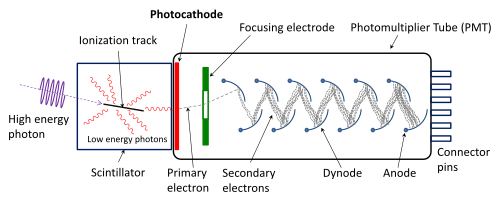
\includegraphics[width=0.7\textwidth]{Images/PhotoMultiplierTubeAndScintillator.png}
  \caption{Schéma global d’un scintillateur couplé à un photomultiplicateur}
  \label{fig:pm_scintillator}
\end{figure}

\textbf{Structure}
Ce tube sous vide comporte une photocathode et une série de dynodes en cascade. La photocathode convertit les photons incidents en électrons par effet photoélectrique. Ces électrons sont ensuite accélérés et multipliés à chaque dynode par émission secondaire, aboutissant à un signal final amplifié de $10^6$ à $10^{10}$ électrons collectés à l'anode.

\textbf{Caractéristiques et limitations}
Les PM présentent une excellente linéarité, une faible contribution au bruit, et une grande rapidité (réponse temporelle de quelques ns). Cependant, ils sont sensibles aux champs magnétiques, nécessitent une alimentation haute tension (HT) (typiquement 1500 V), et doivent être protégés de la lumière ambiante pour éviter les dommages. Le bruit de fond (courant d'obscurité) provient principalement de l'émission thermique d'électrons à la photocathode, mais reste négligeable pour la détection de signaux intenses comme ceux des muons cosmiques.

\begin{remarque}
\textbf{Synthèse~:} Les photomultiplicateurs (PM) offrent une conversion et une amplification très efficaces de la lumière en signal électrique. Toutefois, leur fonctionnement impose des contraintes importantes, notamment une forte dépendance à des tensions d’alimentation élevées et une sensibilité accrue aux perturbations environnementales, susceptibles d’amplifier des signaux parasites.
\end{remarque}


\subsection{Chaîne électronique}

% --- ENCADRÉ DÉBUT ---

\vspace{1em}
\begin{center}
\begin{tcolorbox}[colback=blue!5!white, colframe=blue!60!black, title=Principe de la chaîne électronique]
La chaîne électronique traite, filtre et sélectionne les signaux détectés pour isoler les événements pertinents, optimisant ainsi le rapport signal/bruit.
\end{tcolorbox}
\end{center}

\begin{figure}[H]
  \centering
  \includegraphics[width=0.7\textwidth]{Images/Montage_Electrique.png}
  \caption{Photo des principaux modules électroniques utilisés.}
  \label{fig:photo_instruments}
\end{figure}

% --- FIN ENCADRÉ DÉBUT ---

\begin{center}
\begin{tabular}{|l|p{12cm}|}
\hline
\textbf{Instrument utilisés} & \textbf{Rôle dans l’expérience} \\
\hline
Générateur HT & Alimente les PM avec une tension réglable pour ajuster le gain. \\
\hline
Circuit RC (filtre) & Supprime la composante continue, laisse passer les impulsions rapides. \\
\hline
Amplificateur & Augmente l’amplitude des signaux du PM. \\
\hline
Discriminateur & Ne laisse passer que les impulsions franchissant un seuil défini. \\
\hline
Retardateur & Décale un signal pour synchroniser ou tester les coïncidences fortuites. \\
\hline
Module de coïncidence & Sélectionne les événements simultanés sur plusieurs détecteurs. \\
\hline
Compteur & Compte les impulsions de coïncidence. \\
\hline
Oscilloscope & Visualise les signaux pour réglages et vérifications. \\
\hline
TAC & Convertit un délai entre deux signaux en tension. \\
\hline
\end{tabular}
\end{center}

\begin{remarque}
\textbf{Synthèse~:} La chaîne électronique joue un rôle essentiel dans l’extraction des signaux utiles, leur traitement et leur analyse. Il s'agit d'optimiser les parametres de tout ces composants pour maximiser la qualité des données collectées.
\end{remarque}


\section{Étude du signal}
\subsection{Caractérisation temporelle du signal d’un muon}

% --- ENCADRÉ DÉBUT ---


\begin{center}
\begin{tcolorbox}[colback=blue!5!white, colframe=blue!60!black, title=Principe de l’étude du signal]
L’étude du signal issu de la détection d’un muon cosmique à l’aide d’un scintillateur plastique permet d’accéder à des informations précieuses sur la dynamique de la chaîne d’acquisition. Il s’agit d’analyser la forme, l’amplitude et la dépendance du signal détecté pour optimiser les réglages et garantir la qualité des mesures.
\end{tcolorbox}
\end{center}

% --- FIN ENCADRÉ DÉBUT ---

\begin{figure}[H]
  \centering
  

\tikzset{every picture/.style={line width=0.75pt}} %set default line width to 0.75pt        

\begin{tikzpicture}[x=0.75pt,y=0.75pt,yscale=-1,xscale=1]
%uncomment if require: \path (0,300); %set diagram left start at 0, and has height of 300

%Shape: Parallelogram [id:dp35301618885454245] 
\draw  [fill={rgb, 255:red, 155; green, 155; blue, 155 }  ,fill opacity=1 ][line width=0.75]  (234.63,54.2) -- (74.3,54.2) -- (143.01,66.72) -- (303.34,66.72) -- cycle ;
%Flowchart: Direct Access Storage [id:dp1191186204993182] 
\draw  [fill={rgb, 255:red, 74; green, 144; blue, 226 }  ,fill opacity=1 ][line width=0.75]  (327.9,63) -- (348.34,63) .. controls (351.38,63) and (353.84,59.45) .. (353.84,55.06) .. controls (353.84,50.67) and (351.38,47.12) .. (348.34,47.12) -- (327.9,47.12)(322.4,55.06) .. controls (322.4,59.45) and (324.86,63) .. (327.9,63) .. controls (330.94,63) and (333.4,59.45) .. (333.4,55.06) .. controls (333.4,50.67) and (330.94,47.12) .. (327.9,47.12) .. controls (324.86,47.12) and (322.4,50.67) .. (322.4,55.06) ;
%Shape: Triangle [id:dp5943862032297149] 
\draw  [fill={rgb, 255:red, 155; green, 155; blue, 155 }  ,fill opacity=1 ][line width=0.75]  (328.02,55.6) -- (302.35,66.73) -- (234.63,54.2) -- cycle ;

%Shape: Parallelogram [id:dp695492867171323] 
\draw  [fill={rgb, 255:red, 155; green, 155; blue, 155 }  ,fill opacity=1 ] (234.63,74.2) -- (74.3,74.2) -- (143.01,86.72) -- (303.34,86.72) -- cycle ;
%Flowchart: Direct Access Storage [id:dp5221446506871552] 
\draw  [fill={rgb, 255:red, 74; green, 144; blue, 226 }  ,fill opacity=1 ] (327.9,83) -- (348.34,83) .. controls (351.38,83) and (353.84,79.45) .. (353.84,75.06) .. controls (353.84,70.67) and (351.38,67.12) .. (348.34,67.12) -- (327.9,67.12)(322.4,75.06) .. controls (322.4,79.45) and (324.86,83) .. (327.9,83) .. controls (330.94,83) and (333.4,79.45) .. (333.4,75.06) .. controls (333.4,70.67) and (330.94,67.12) .. (327.9,67.12) .. controls (324.86,67.12) and (322.4,70.67) .. (322.4,75.06) ;
%Shape: Triangle [id:dp6049217793564252] 
\draw  [fill={rgb, 255:red, 155; green, 155; blue, 155 }  ,fill opacity=1 ] (328.02,75.6) -- (302.35,86.73) -- (234.63,74.2) -- cycle ;

%Shape: Parallelogram [id:dp7041756667150763] 
\draw  [fill={rgb, 255:red, 155; green, 155; blue, 155 }  ,fill opacity=1 ] (234.63,94.2) -- (74.3,94.2) -- (143.01,106.72) -- (303.34,106.72) -- cycle ;
%Flowchart: Direct Access Storage [id:dp33919363706983496] 
\draw  [fill={rgb, 255:red, 74; green, 144; blue, 226 }  ,fill opacity=1 ] (327.9,103) -- (348.34,103) .. controls (351.38,103) and (353.84,99.45) .. (353.84,95.06) .. controls (353.84,90.67) and (351.38,87.12) .. (348.34,87.12) -- (327.9,87.12)(322.4,95.06) .. controls (322.4,99.45) and (324.86,103) .. (327.9,103) .. controls (330.94,103) and (333.4,99.45) .. (333.4,95.06) .. controls (333.4,90.67) and (330.94,87.12) .. (327.9,87.12) .. controls (324.86,87.12) and (322.4,90.67) .. (322.4,95.06) ;
%Shape: Triangle [id:dp803626559288593] 
\draw  [fill={rgb, 255:red, 155; green, 155; blue, 155 }  ,fill opacity=1 ] (328.02,95.6) -- (302.35,106.73) -- (234.63,94.2) -- cycle ;

%Curve Lines [id:da23112739158493478] 
\draw    (353.84,55.06) .. controls (393.84,25.06) and (394.24,101.52) .. (434.24,71.52) ;
%Curve Lines [id:da07382068018293464] 
\draw    (353.84,75.06) .. controls (393.84,45.06) and (394.24,101.52) .. (434.24,71.52) ;
%Curve Lines [id:da46913396438255406] 
\draw    (353.84,95.06) .. controls (393.84,65.06) and (394.24,101.52) .. (434.24,71.52) ;
%Shape: Rectangle [id:dp1854672149647154] 
\draw  [fill={rgb, 255:red, 255; green, 0; blue, 32 }  ,fill opacity=1 ] (434,51.6) -- (458.24,51.6) -- (458.24,91.6) -- (434,91.6) -- cycle ;
%Straight Lines [id:da7316920119479293] 
\draw    (458.4,71.4) -- (481.44,71.52) ;
%Shape: Frame [id:dp08781099507426449] 
\draw   (482,51.4) -- (552,51.4) -- (552,91.4) -- (482,91.4) -- cycle(546,57.4) -- (488,57.4) -- (488,85.4) -- (546,85.4) -- cycle ;
%Shape: Rectangle [id:dp8950202022795561] 
\draw   (313.2,116.11) -- (368.64,116.11) -- (368.64,121.89) -- (313.2,121.89) -- cycle ;
%Shape: Rectangle [id:dp4725062366406878] 
\draw   (313.2,121.89) -- (368.64,121.89) -- (368.64,127.68) -- (313.2,127.68) -- cycle ;
%Shape: Rectangle [id:dp7793332758957106] 
\draw   (313.2,110.32) -- (368.64,110.32) -- (368.64,116.11) -- (313.2,116.11) -- cycle ;

%Straight Lines [id:da3286199203085991] 
\draw    (340.64,102.64) -- (340.64,110.2) ;
%Straight Lines [id:da5977149050528532] 
\draw    (340.4,82.89) -- (340.49,87.27) ;
%Straight Lines [id:da8284872647272457] 
\draw    (339.78,62.58) -- (339.87,66.97) ;

% Text Node
\draw (487.2,31.2) node [anchor=north west][inner sep=0.75pt]   [align=left] {{\tiny Oscilloscope}};
% Text Node
\draw (415.6,31.2) node [anchor=north west][inner sep=0.75pt]   [align=left] {{\tiny Amplificateur}};
% Text Node
\draw (323.8,26.55) node [anchor=north west][inner sep=0.75pt]   [align=left] {{\tiny PMTs}};
% Text Node
\draw (186.4,28.2) node [anchor=north west][inner sep=0.75pt]   [align=left] {{\tiny Scintillateurs}};
% Text Node
\draw (310.8,133.94) node [anchor=north west][inner sep=0.75pt]   [align=left] {{\tiny Haute Tension}};


\end{tikzpicture}

  \caption{Schéma de la chaîne électronique utilisée pour visualiser le signal d’un muon cosmique.}
  \label{fig:scintillator}
\end{figure}

Le signal typique, mesuré à l’oscilloscope, présente une décroissance exponentielle caractéristique, liée à la désexcitation des molécules du scintillateur, ainsi qu’une remontée associée à la réponse de l’électronique (constante de temps RC).

L’ajustement de deux exponentielles (descente et montée) sur les données expérimentales permet d’extraire deux constantes de temps :
\begin{itemize}
    \item $\tau_{\text{scint}}$ : constante de décroissance du scintillateur plastique (processus de désexcitation)
    \item $\tau_{RC}$ : constante de temps de la chaîne électronique (filtrage RC)
\end{itemize}

\begin{figure}[H]
    \centering
    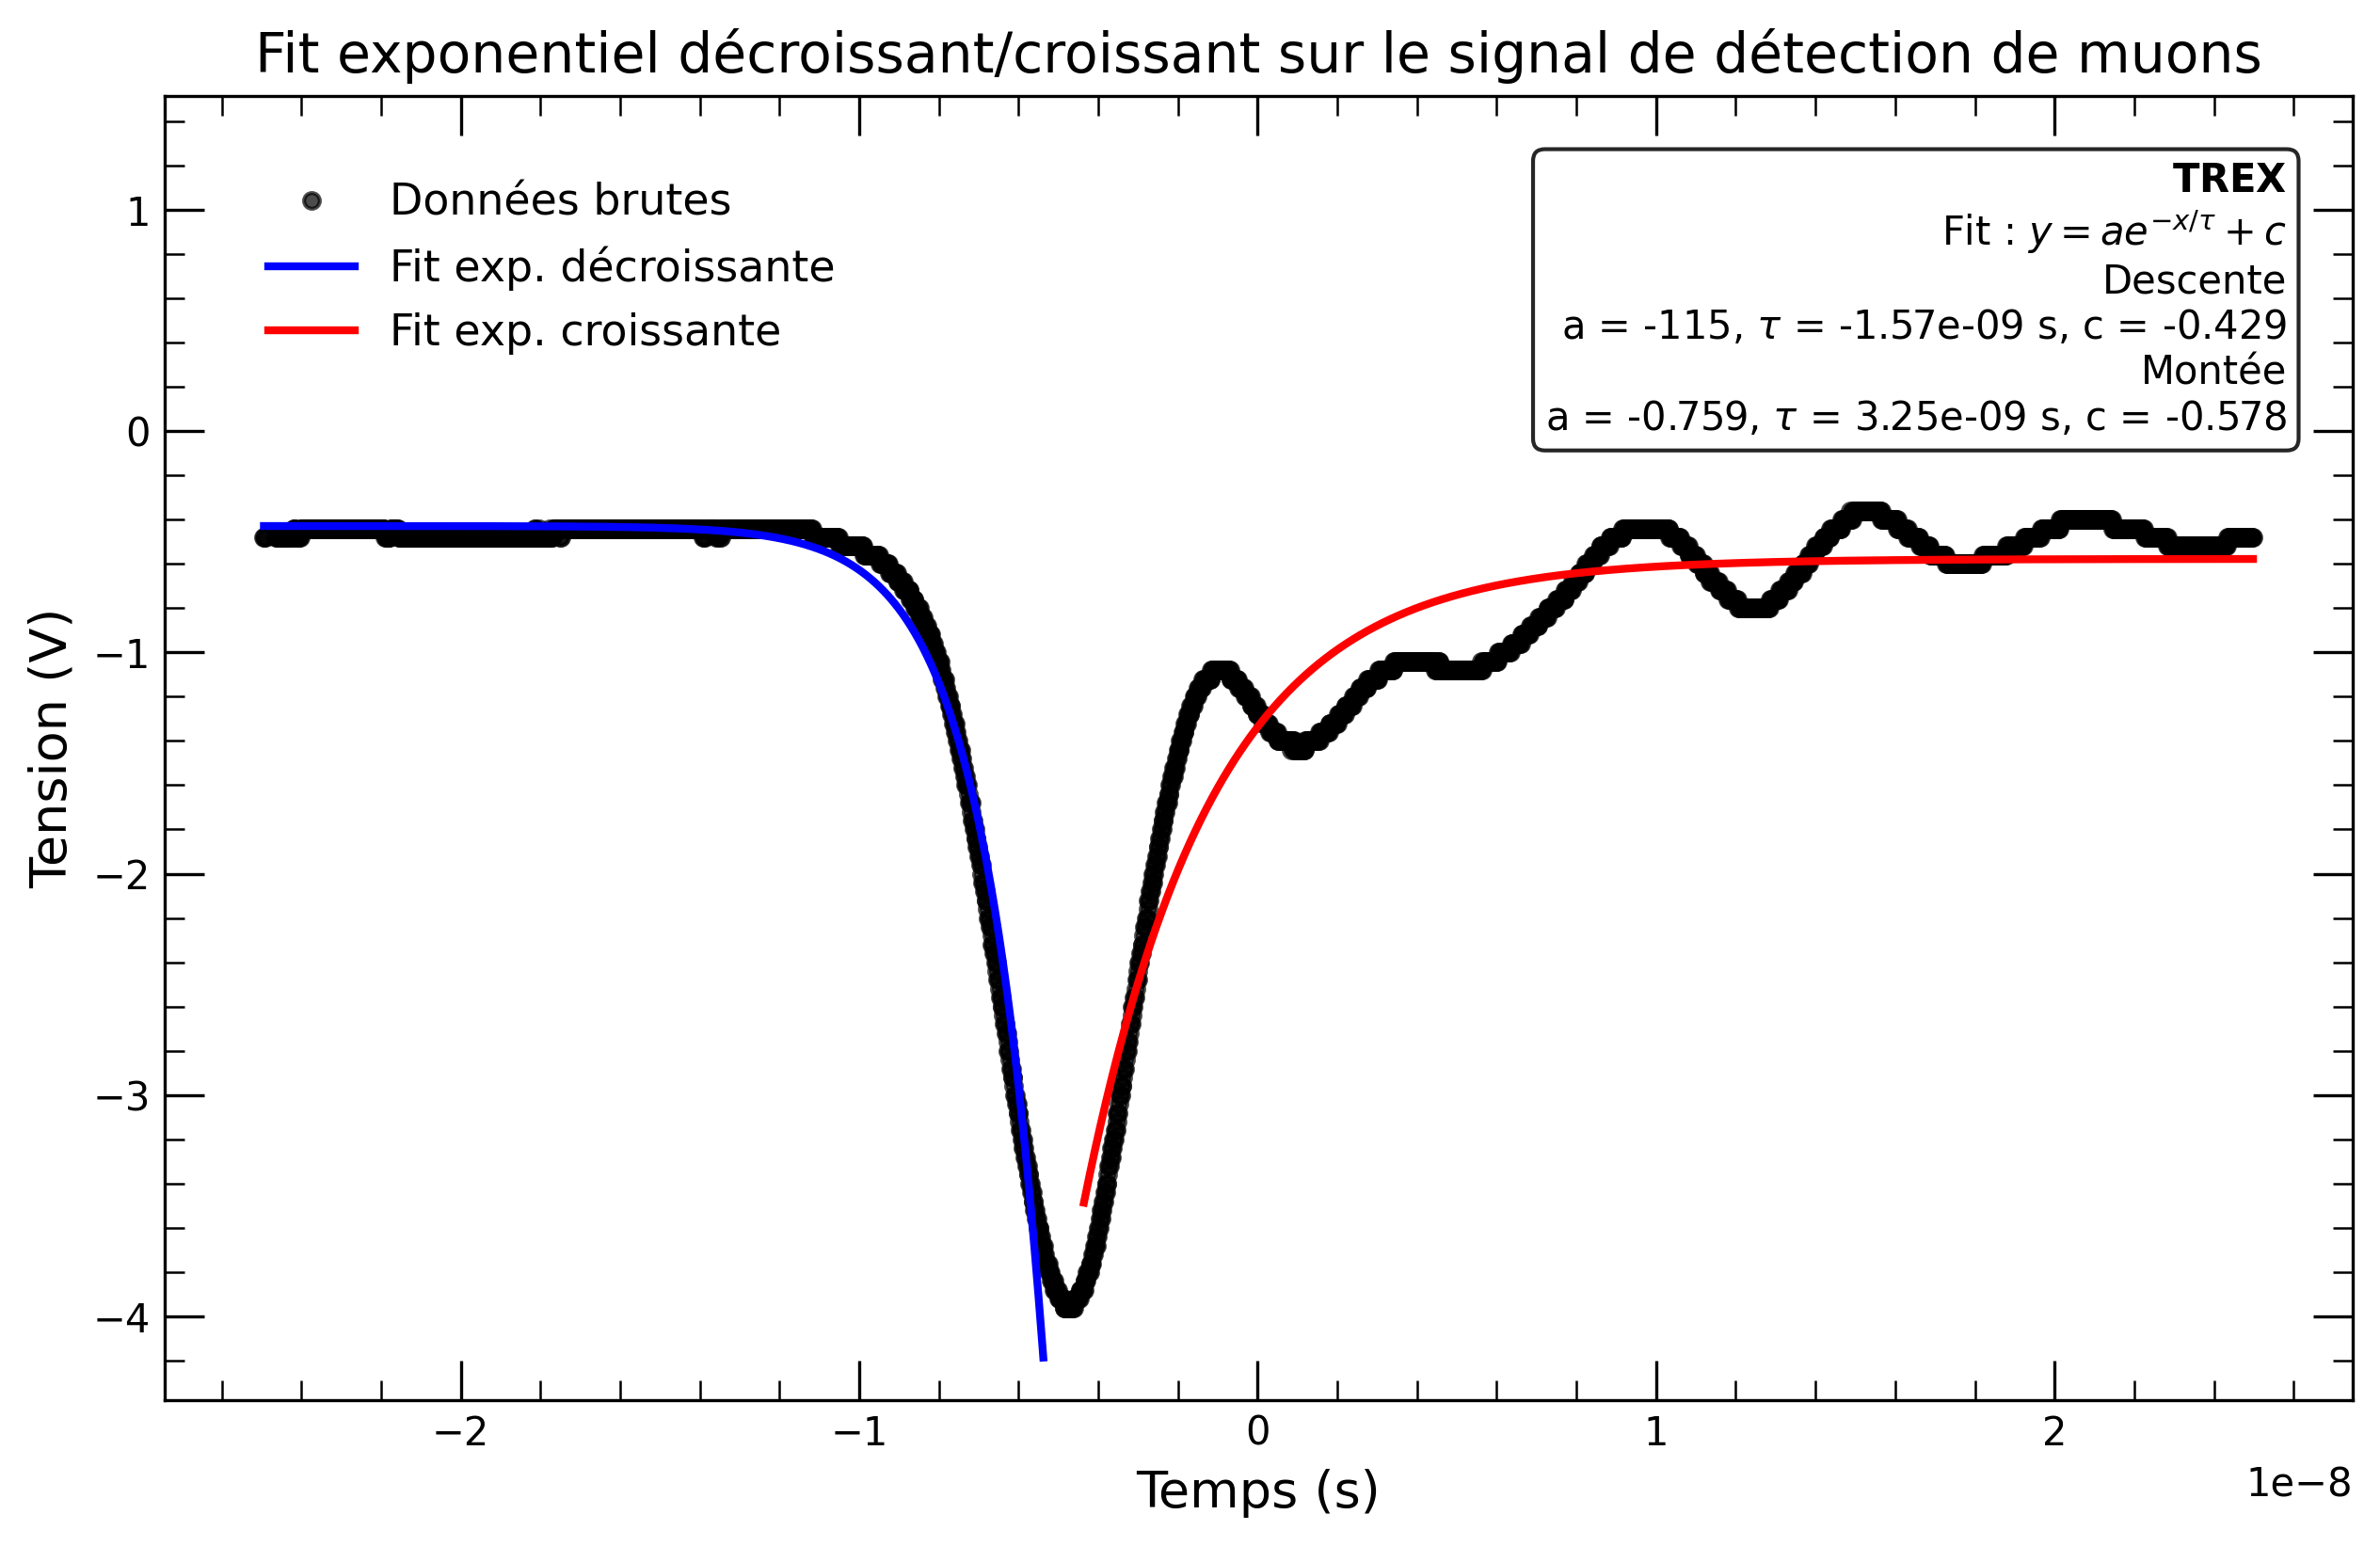
\includegraphics[width=1\textwidth]{Images/Desexitation_Scintillateur_2.png}
    \caption{Exemple de signal mesuré sur un muon cosmique, avec ajustements exponentiels sur la descente et la montée.}
    \label{fig:signal-muon}
\end{figure}

\begin{remarque}
\textbf{Synthèse~:} L’ajustement exponentiel du signal mesuré a permis d’extraire deux constantes caractéristiques~: $\tau_{\text{scint}} = 1{,}57$~ns (désexcitation du scintillateur) et $\tau_{RC} = 3{,}25$~ns (réponse de la chaîne électronique). La valeur obtenue pour $\tau_{\text{scint}}$ est parfaitement cohérente avec les propriétés attendues pour un scintillateur plastique, confirmant l’analyse temporelle réalisée.
Le même processus a été appliqué aux autres scintillateurs. Des constantes similaires ont été obtenues, confirmant la nature des scintillateurs plastiques utilisés.
\end{remarque}

\newpage

\subsection{Optimisation conjointe de la haute tension et du seuil du discriminateur}

% --- ENCADRÉ DÉBUT ---

\vspace{1em}
\begin{center}
\begin{tcolorbox}[colback=blue!5!white, colframe=blue!60!black, title=Optimisation conjointe des réglages électroniques]
Pour maximiser la détection des muons cosmiques tout en minimisant le bruit de fond, il est essentiel d’ajuster simultanément la HT appliquée au PM et le seuil du discriminateur.
\end{tcolorbox}
\end{center}

% --- FIN ENCADRÉ DÉBUT ---

\textbf{Démarche expérimentale~:}
Pour chaque scintillateur, nous avons mesuré le nombre d’événements détectés en fonction du seuil du discriminateur, pour plusieurs valeurs de haute-tension. Cette cartographie est censée permettre d’identifier la zone optimale où le taux de détection des muons est maximal et le bruit de fond minimal.

\begin{figure}[H]
  \centering
  

\tikzset{every picture/.style={line width=0.75pt}} %set default line width to 0.75pt        

\begin{tikzpicture}[x=0.75pt,y=0.75pt,yscale=-1,xscale=1]
%uncomment if require: \path (0,300); %set diagram left start at 0, and has height of 300

%Shape: Parallelogram [id:dp6153094668241826] 
\draw  [fill={rgb, 255:red, 155; green, 155; blue, 155 }  ,fill opacity=1 ][line width=0.75]  (234.63,54.2) -- (74.3,54.2) -- (143.01,66.72) -- (303.34,66.72) -- cycle ;
%Flowchart: Direct Access Storage [id:dp057480924744088946] 
\draw  [fill={rgb, 255:red, 74; green, 144; blue, 226 }  ,fill opacity=1 ][line width=0.75]  (327.9,63) -- (348.34,63) .. controls (351.38,63) and (353.84,59.45) .. (353.84,55.06) .. controls (353.84,50.67) and (351.38,47.12) .. (348.34,47.12) -- (327.9,47.12)(322.4,55.06) .. controls (322.4,59.45) and (324.86,63) .. (327.9,63) .. controls (330.94,63) and (333.4,59.45) .. (333.4,55.06) .. controls (333.4,50.67) and (330.94,47.12) .. (327.9,47.12) .. controls (324.86,47.12) and (322.4,50.67) .. (322.4,55.06) ;
%Shape: Triangle [id:dp281161219892323] 
\draw  [fill={rgb, 255:red, 155; green, 155; blue, 155 }  ,fill opacity=1 ][line width=0.75]  (328.02,55.6) -- (302.35,66.73) -- (234.63,54.2) -- cycle ;

%Shape: Parallelogram [id:dp9101804879233704] 
\draw  [fill={rgb, 255:red, 155; green, 155; blue, 155 }  ,fill opacity=1 ] (234.63,74.2) -- (74.3,74.2) -- (143.01,86.72) -- (303.34,86.72) -- cycle ;
%Flowchart: Direct Access Storage [id:dp015646766055150918] 
\draw  [fill={rgb, 255:red, 74; green, 144; blue, 226 }  ,fill opacity=1 ] (327.9,83) -- (348.34,83) .. controls (351.38,83) and (353.84,79.45) .. (353.84,75.06) .. controls (353.84,70.67) and (351.38,67.12) .. (348.34,67.12) -- (327.9,67.12)(322.4,75.06) .. controls (322.4,79.45) and (324.86,83) .. (327.9,83) .. controls (330.94,83) and (333.4,79.45) .. (333.4,75.06) .. controls (333.4,70.67) and (330.94,67.12) .. (327.9,67.12) .. controls (324.86,67.12) and (322.4,70.67) .. (322.4,75.06) ;
%Shape: Triangle [id:dp42632878589040457] 
\draw  [fill={rgb, 255:red, 155; green, 155; blue, 155 }  ,fill opacity=1 ] (328.02,75.6) -- (302.35,86.73) -- (234.63,74.2) -- cycle ;

%Shape: Parallelogram [id:dp08291359315510605] 
\draw  [fill={rgb, 255:red, 155; green, 155; blue, 155 }  ,fill opacity=1 ] (234.63,94.2) -- (74.3,94.2) -- (143.01,106.72) -- (303.34,106.72) -- cycle ;
%Flowchart: Direct Access Storage [id:dp39415762621948935] 
\draw  [fill={rgb, 255:red, 74; green, 144; blue, 226 }  ,fill opacity=1 ] (327.9,103) -- (348.34,103) .. controls (351.38,103) and (353.84,99.45) .. (353.84,95.06) .. controls (353.84,90.67) and (351.38,87.12) .. (348.34,87.12) -- (327.9,87.12)(322.4,95.06) .. controls (322.4,99.45) and (324.86,103) .. (327.9,103) .. controls (330.94,103) and (333.4,99.45) .. (333.4,95.06) .. controls (333.4,90.67) and (330.94,87.12) .. (327.9,87.12) .. controls (324.86,87.12) and (322.4,90.67) .. (322.4,95.06) ;
%Shape: Triangle [id:dp44810110314081986] 
\draw  [fill={rgb, 255:red, 155; green, 155; blue, 155 }  ,fill opacity=1 ] (328.02,95.6) -- (302.35,106.73) -- (234.63,94.2) -- cycle ;

%Curve Lines [id:da8784603980762927] 
\draw    (353.84,55.06) .. controls (393.84,25.06) and (392,102) .. (432,72) ;
%Curve Lines [id:da9313823595606255] 
\draw    (353.84,75.06) .. controls (393.84,45.06) and (392,102) .. (432,72) ;
%Curve Lines [id:da24872657353422778] 
\draw    (353.84,95.06) .. controls (393.84,65.06) and (392,102) .. (432,72) ;
%Shape: Rectangle [id:dp7955377352395961] 
\draw  [fill={rgb, 255:red, 208; green, 2; blue, 27 }  ,fill opacity=1 ] (432,48) -- (456.24,48) -- (456.24,96) -- (432,96) -- cycle ;
%Shape: Frame [id:dp790746320543737] 
\draw   (564,12) -- (634,12) -- (634,52) -- (564,52) -- cycle(628,18) -- (570,18) -- (570,46) -- (628,46) -- cycle ;
%Shape: Rectangle [id:dp8336691747772105] 
\draw   (313.2,116.11) -- (368.64,116.11) -- (368.64,121.89) -- (313.2,121.89) -- cycle ;
%Shape: Rectangle [id:dp6493800754350441] 
\draw   (313.2,121.89) -- (368.64,121.89) -- (368.64,127.68) -- (313.2,127.68) -- cycle ;
%Shape: Rectangle [id:dp7269506258160386] 
\draw   (313.2,110.32) -- (368.64,110.32) -- (368.64,116.11) -- (313.2,116.11) -- cycle ;

%Straight Lines [id:da6829845507956613] 
\draw    (340.64,102.64) -- (340.64,110.2) ;
%Straight Lines [id:da5330000370742687] 
\draw    (340.4,82.89) -- (340.49,87.27) ;
%Straight Lines [id:da5174947670175065] 
\draw    (339.78,62.58) -- (339.87,66.97) ;
%Shape: Rectangle [id:dp7820496204409214] 
\draw  [fill={rgb, 255:red, 74; green, 144; blue, 226 }  ,fill opacity=1 ] (479.76,48) -- (504,48) -- (504,96) -- (479.76,96) -- cycle ;
%Shape: Frame [id:dp44415473016363605] 
\draw   (564,80) -- (634,80) -- (634,120) -- (564,120) -- cycle(628,86) -- (570,86) -- (570,114) -- (628,114) -- cycle ;
%Curve Lines [id:da7027674246282678] 
\draw    (504,72) .. controls (544,42) and (524.71,27.29) .. (564,36) ;
%Curve Lines [id:da161234971098009] 
\draw    (504,72) .. controls (544,42) and (524,126) .. (564,96) ;
%Straight Lines [id:da2592906745330712] 
\draw    (456,60) -- (492,60) ;
\draw [shift={(492,60)}, rotate = 0] [color={rgb, 255:red, 0; green, 0; blue, 0 }  ][fill={rgb, 255:red, 0; green, 0; blue, 0 }  ][line width=0.75]      (0, 0) circle [x radius= 3.35, y radius= 3.35]   ;
%Straight Lines [id:da4896356965331372] 
\draw    (456,72) -- (492,72) ;
\draw [shift={(492,72)}, rotate = 0] [color={rgb, 255:red, 0; green, 0; blue, 0 }  ][fill={rgb, 255:red, 0; green, 0; blue, 0 }  ][line width=0.75]      (0, 0) circle [x radius= 3.35, y radius= 3.35]   ;
%Straight Lines [id:da963095590048375] 
\draw    (456,84) -- (492,84) ;
\draw [shift={(492,84)}, rotate = 0] [color={rgb, 255:red, 0; green, 0; blue, 0 }  ][fill={rgb, 255:red, 0; green, 0; blue, 0 }  ][line width=0.75]      (0, 0) circle [x radius= 3.35, y radius= 3.35]   ;

% Text Node
\draw (574,17) node [anchor=north west][inner sep=0.75pt]   [align=left] {{\tiny \textbf{Oscilloscope}}};
% Text Node
\draw (420,27) node [anchor=north west][inner sep=0.75pt]   [align=left] {{\tiny Amplificateur}};
% Text Node
\draw (328.8,27) node [anchor=north west][inner sep=0.75pt]   [align=left] {{\tiny PMTs}};
% Text Node
\draw (186.4,28.2) node [anchor=north west][inner sep=0.75pt]   [align=left] {{\tiny Scintillateurs}};
% Text Node
\draw (310,130) node [anchor=north west][inner sep=0.75pt]   [align=left] {{\tiny Haute Tension}};
% Text Node
\draw (465,110) node [anchor=north west][inner sep=0.75pt]   [align=left] {{\tiny Discriminateur}};
% Text Node
\draw (578,97) node [anchor=north west][inner sep=0.75pt]  [font=\footnotesize] [align=left] {{\fontfamily{pcr}\selectfont {\footnotesize \textcolor[rgb]{1,0,0}{000}}}};
% Text Node
\draw (607,96) node [anchor=north west][inner sep=0.75pt]  [font=\footnotesize] [align=left] {{\fontfamily{pcr}\selectfont {\tiny \textcolor[rgb]{1,0,0}{600s}}}};
% Text Node
\draw (572,81) node [anchor=north west][inner sep=0.75pt]   [align=left] {{\tiny \textbf{Compteur}}};


\end{tikzpicture}

  \caption{Schéma de la chaîne électronique utilisée pour faire varier la haute tension et le seuil du discriminateur.}
  \label{fig:variation_seuil}
\end{figure}

% Trois figures séparées pour chaque scintillateur

\begin{figure}[H]
    \centering
    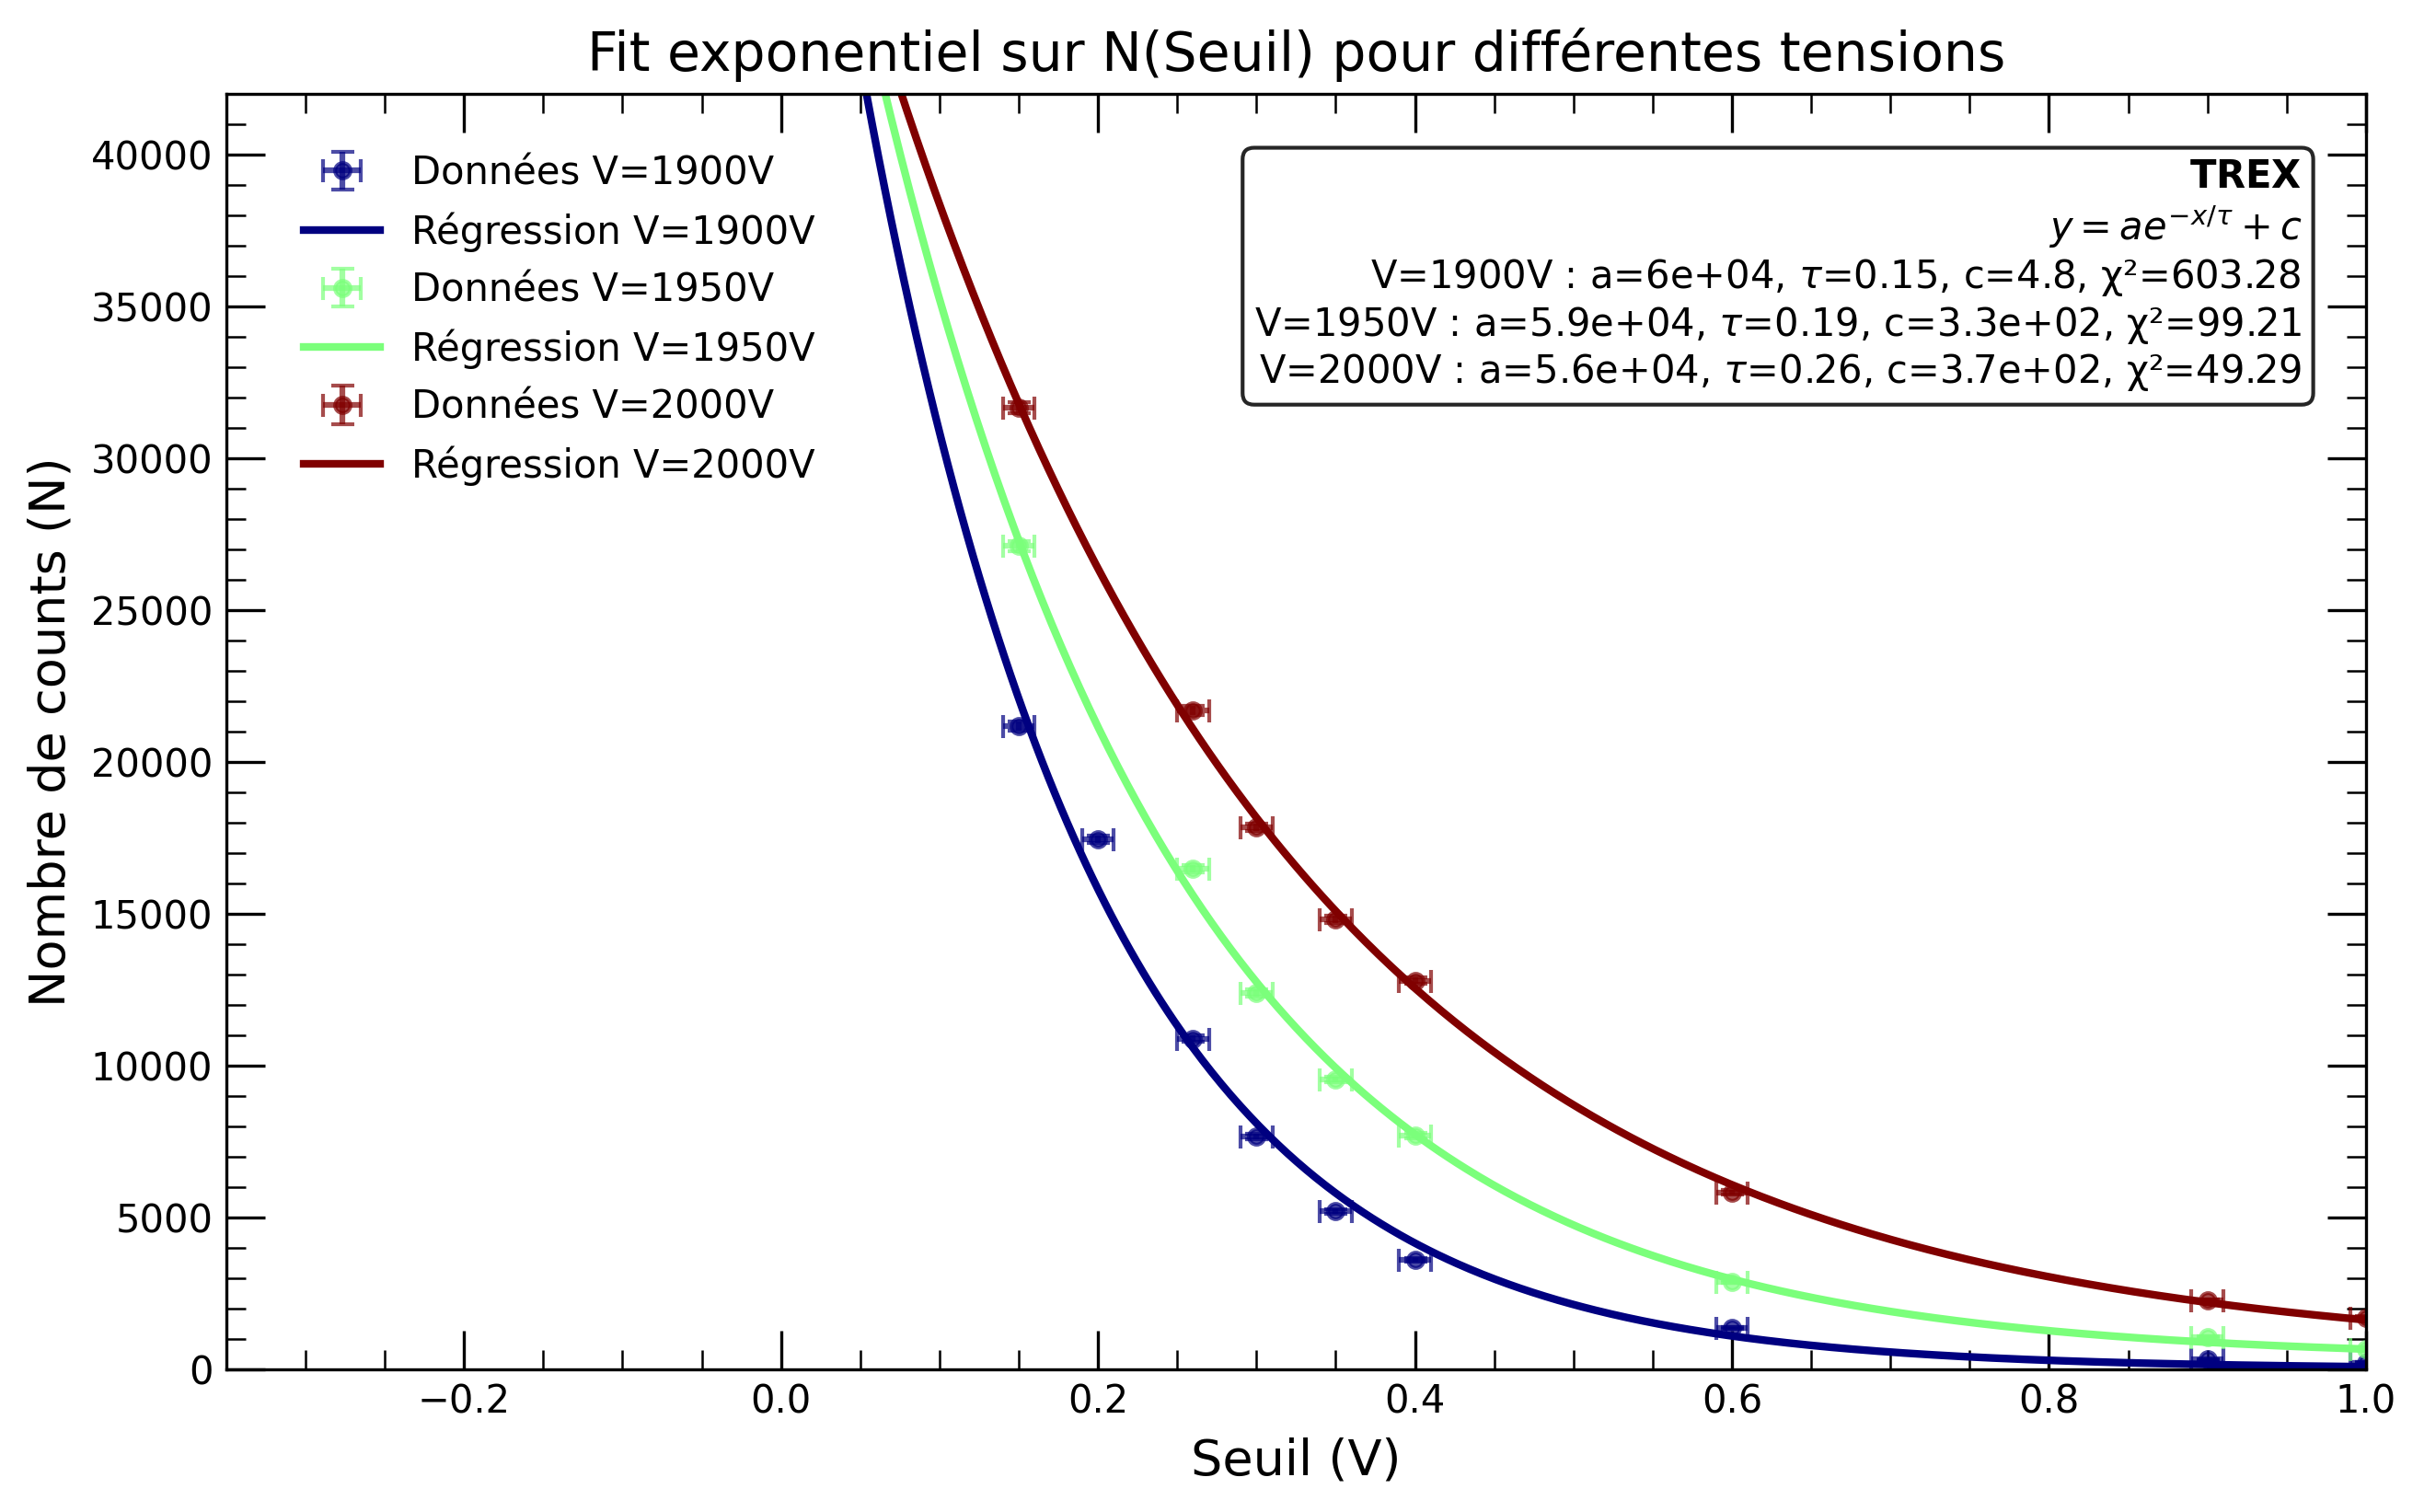
\includegraphics[width=0.7\textwidth]{Images/Threshold_Scintillateur_1.png}
    \caption{Nombre d’événements détectés en fonction du seuil pour différentes HT (Scintillateur 1).
    On observe l'absence de palier net, ce qui rend l'optimisation difficile, en plus d'un nombre de count anormalement élevé.}
    \label{fig:optimisation_scint1}
\end{figure}

\begin{figure}[H]
  \begin{minipage}{0.49\textwidth}
    \centering
    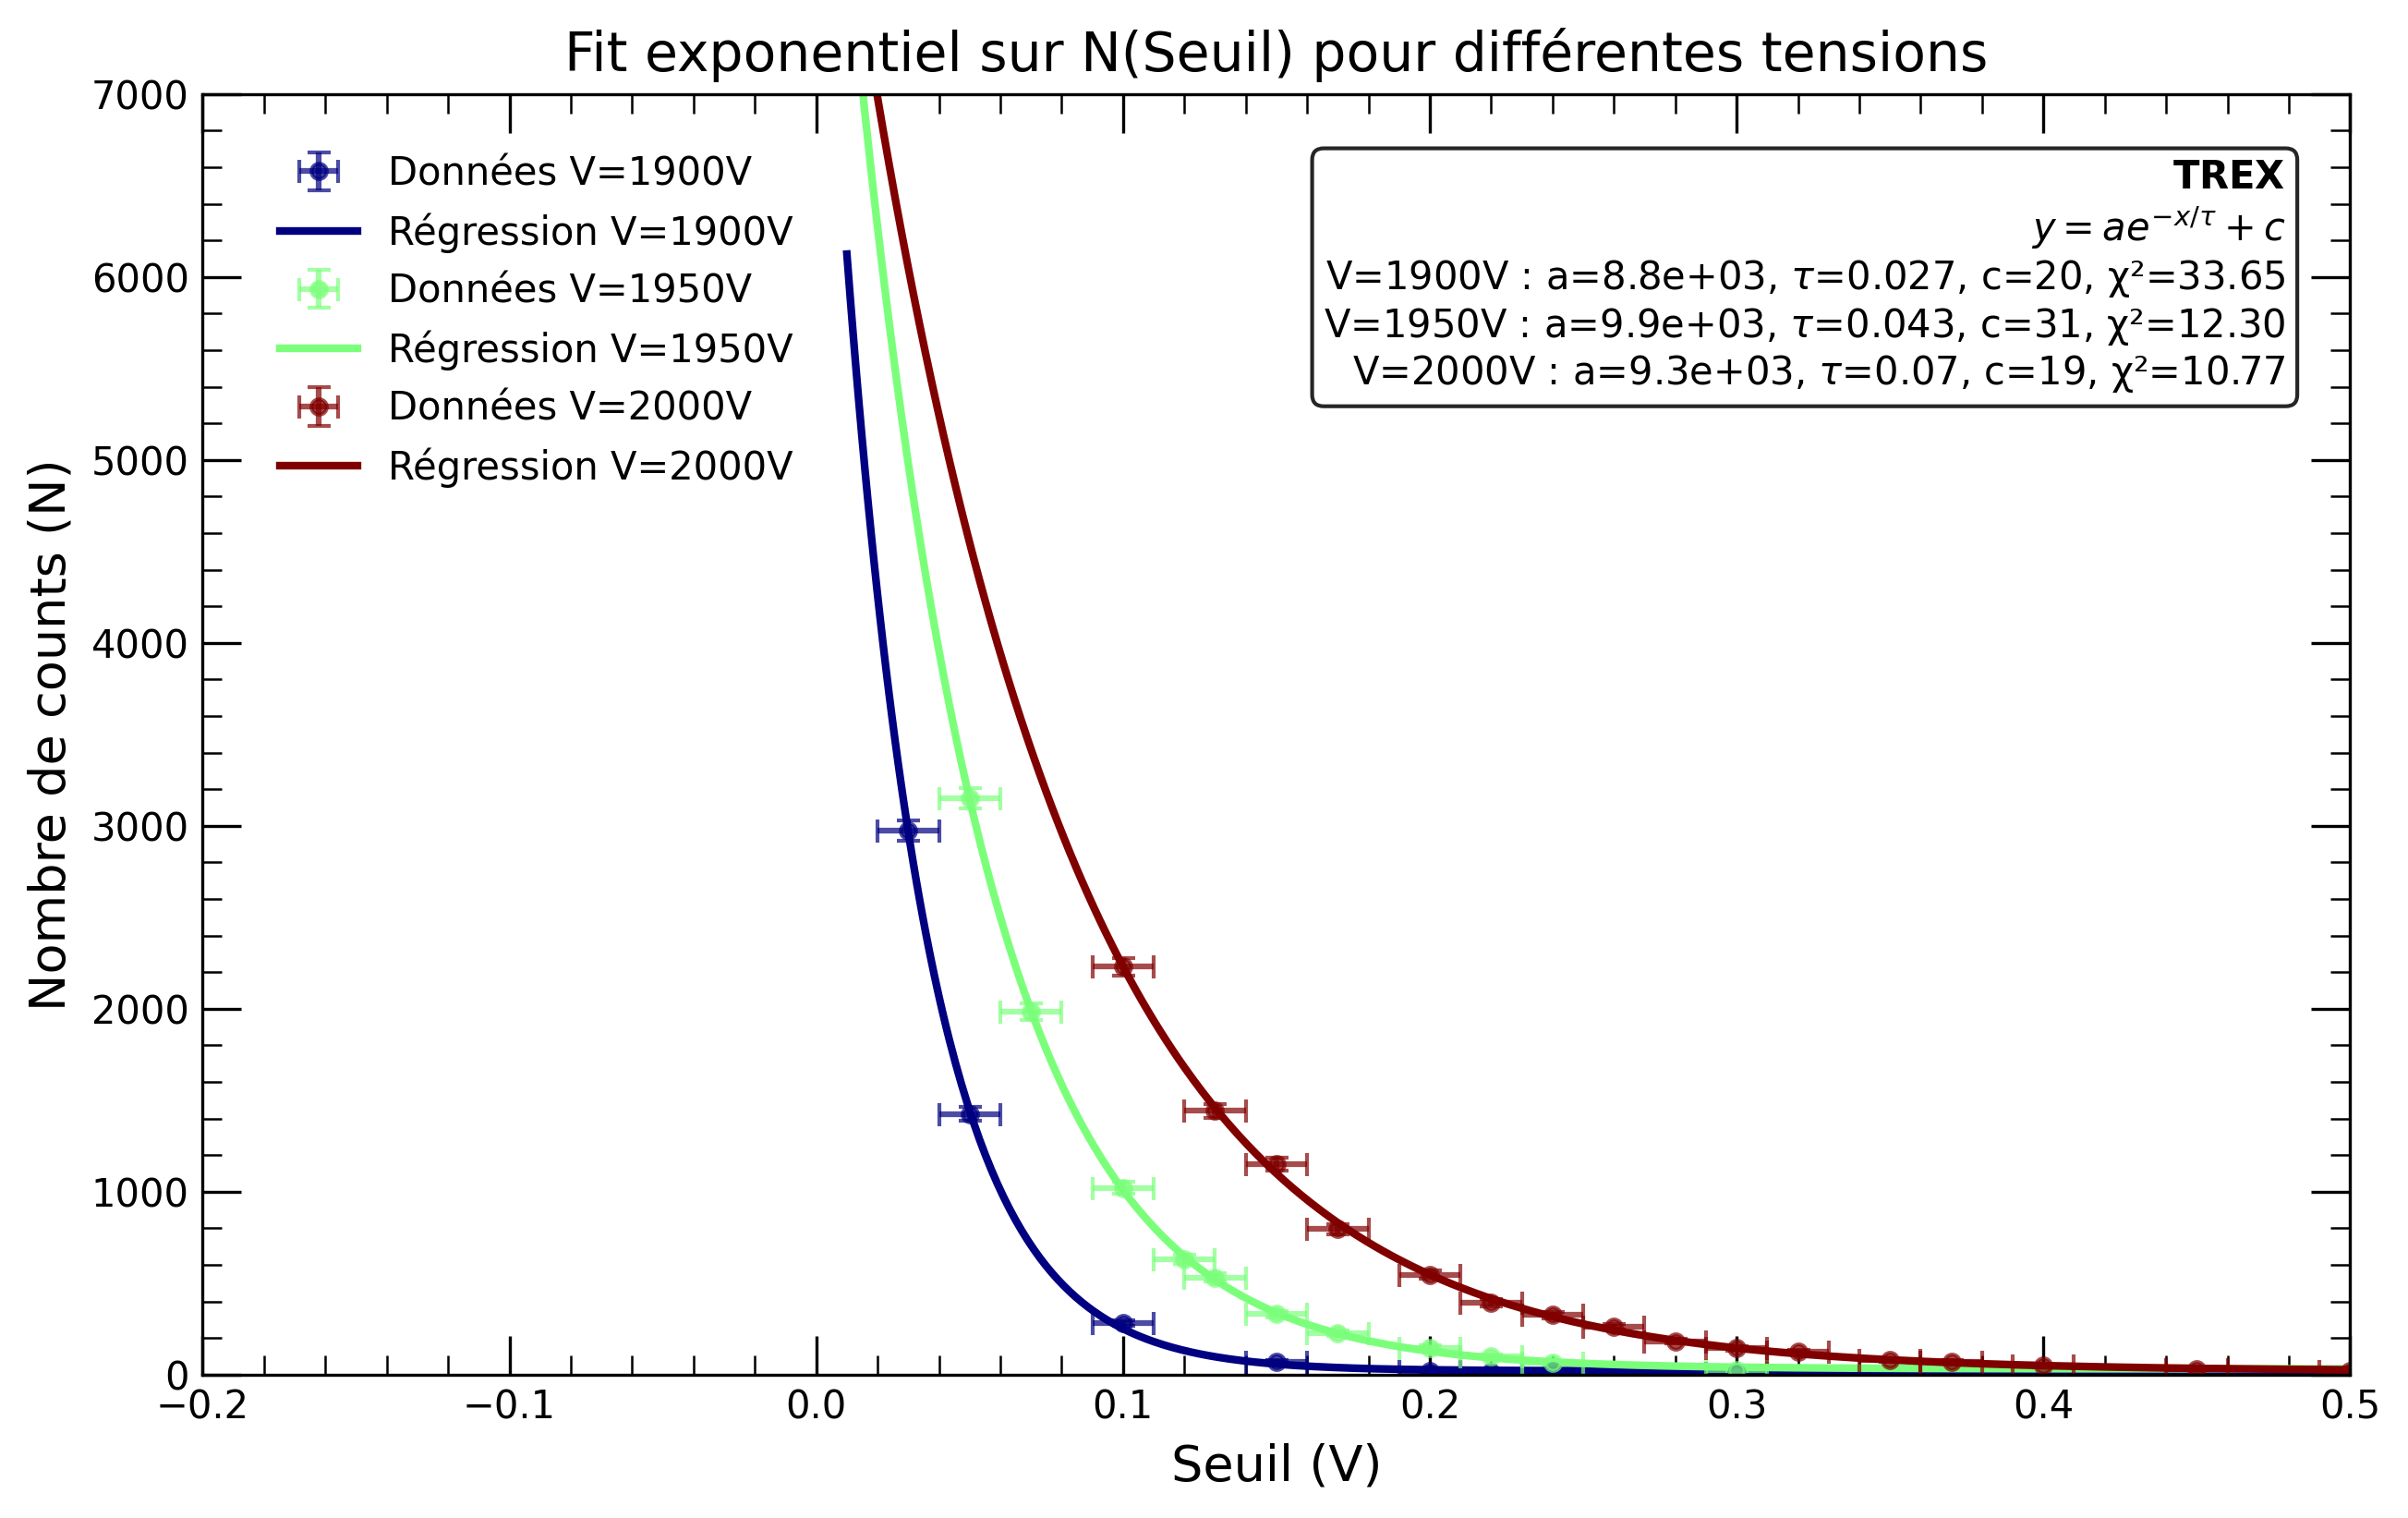
\includegraphics[width=0.95\textwidth]{Images/Threshold_Scintillateur_2.png}
    \caption{Nombre d’événements détectés en fonction du seuil pour différentes HT (Scintillateur 2)
    Les valeurs de HT utilisées sont 2000~V (rouge), 1950~V(vert) et 1900~V (bleu).
    On observe l'absence de palier net, ce qui rend l'optimisation difficile.}
    \label{fig:optimisation_scint2}
  \end{minipage}
  \hfill
  \begin{minipage}{0.49\textwidth}
    \centering
    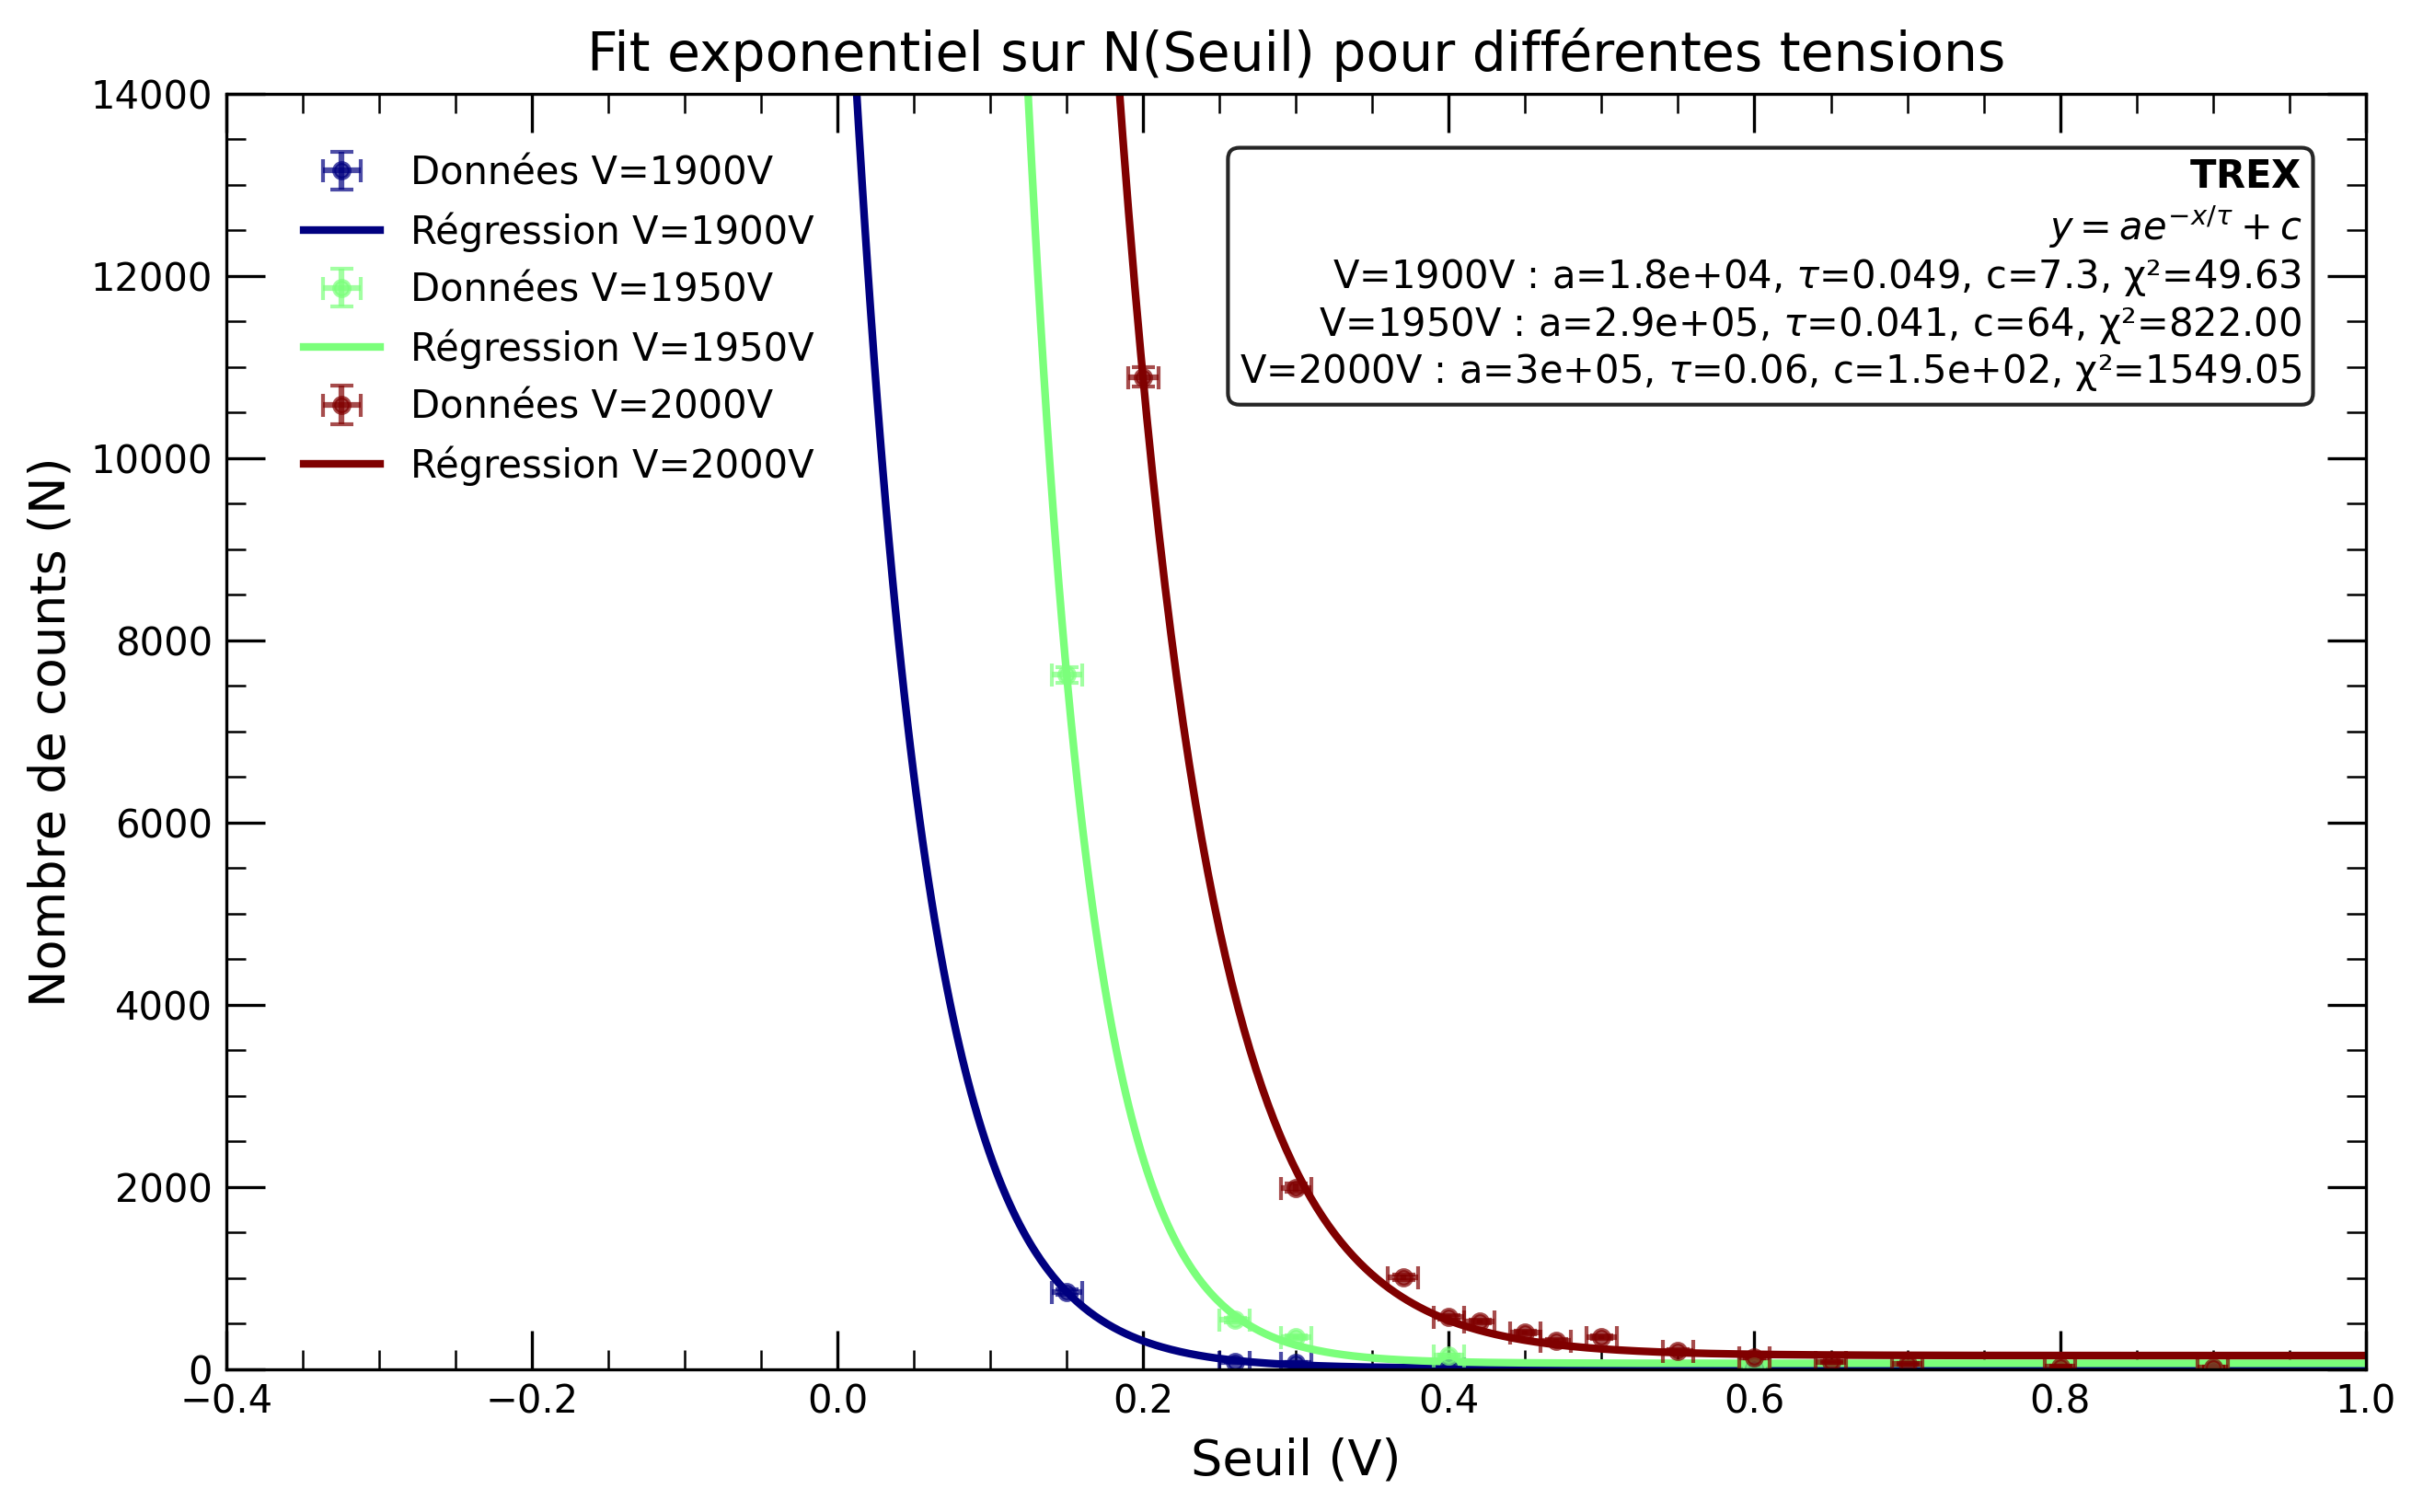
\includegraphics[width=0.95\textwidth]{Images/Threshold_Scintillateur_3.png}
    \caption{Nombre d’événements détectés en fonction du seuil pour différentes HT (Scintillateur 3).
    Les valeurs de HT utilisées sont 2000~V (rouge), 1950~V(vert) et 1900~V (bleu).
    On observe l'absence de palier net, ce qui rend l'optimisation difficile.}
    \label{fig:optimisation_scint3}

  \end{minipage}
\end{figure}

% --- ENCADRÉ PROBLÈMES DÉBUT ---

\begin{center}
\begin{tcolorbox}[colback=red!5!white, colframe=red!80!black, title=Problèmes rencontrés lors de l'optimisation]
Lors de l’optimisation conjointe du seuil et de la haute tension, plusieurs difficultés majeures ont été rencontrées :
\begin{itemize}
    \item \textbf{Comptes très différents entre scintillateurs} : pour un même seuil, on observe parfois un facteur 20 entre deux scintillateurs (ex : 40 000 pour l’un, 2 000 pour l’autre).
    \item \textbf{Absence de palier net} : il était difficile d’identifier un palier clair dans la courbe de comptage ; lorsque l’on s’en approchait, le nombre de counts devenait trop faible pour modéliser correctement la zone.
    \item \textbf{Durée d’acquisition limitée} : chaque point correspond à un count par minute ; augmenter la durée pour améliorer la statistique aurait nécessité un temps d’acquisition très long (nombre de seuils $\times$ temps d’acquisition $\times$ 3 scintillateurs $\times$ nombre de tensions).
    \item \textbf{Variabilité d’un jour à l’autre} : les mesures n’étaient pas reproductibles d’un jour à l’autre, traduisant une grande sensibilité aux réglages de HT et de seuil.
    \item \textbf{Ratio signal/bruit inattendu} : on s’attendait à ce que le ratio (nombre de vrais muons détectés divisé par le nombre de fausses coïncidences) soit plus grand pour 3 scintillateurs que pour 2, mais nous avons observé l’inverse. Cela peut s’expliquer par le très faible nombre de détections, malgré un temps d’acquisition de 10 minutes, ce qui augmente l’incertitude statistique et peut fausser le ratio mesuré. Il est aussi possible qu’une défaillance ou une usure d'un des scintillateurs ait fortement réduit la zone de détection réelle (plus petite que la surface du scintillateur), ce qui diminue le nombre de “vrais” muons détectés. À noter que pour les mesures à 2 scintillateurs, nous avions sélectionné les deux détecteurs les plus efficaces, ce qui a permis d’obtenir de meilleures données.
\end{itemize}
Ces limitations ont rendu l’optimisation fine difficile et expliquent la dispersion des résultats.
\end{tcolorbox}
\end{center}

% --- Synthèse résultats coïncidences ---

\begin{remarque}
\textbf{Synthèse~:} Après optimisation, les réglages retenus pour chaque scintillateur sont les suivants :
\begin{itemize}
    \item \textbf{Scintillateur 1 :} Haute tension (HT) = 2000~V, seuil du discriminateur = 0.45~V.
    \item \textbf{Scintillateur 2 :} Haute tension (HT) = 2050~V, seuil du discriminateur = 0.05~V.
    \item \textbf{Scintillateur 3 :} Haute tension (HT) = 2060~V, seuil du discriminateur = 0.3~V.
\end{itemize}
Ces valeurs permettent de maximiser le taux de détection des muons tout en minimisant le bruit de fond. Elles permettent aussi d'avoir un nombre de count similaire entyre détecteurs.
\end{remarque}

\newpage

\section{Détection par coïncidence}

\subsection{Principe de coïncidence}



\begin{center}
\begin{tcolorbox}[colback=blue!5!white, colframe=blue!60!black, title=Principe de la coïncidence]
Seuls les muons, très pénétrants, peuvent traverser plusieurs détecteurs alignés en quasi-ligne droite et produire des signaux quasi simultanés dans chacun. Les bruits aléatoires, eux, n’ont qu’une probabilité infime d’apparaître exactement en même temps dans deux détecteurs distincts.
\end{tcolorbox}
\end{center}

\begin{figure}[H]
  \begin{minipage}
    [t]{0.45\textwidth}
    \centering
    

\tikzset{every picture/.style={line width=0.75pt}} %set default line width to 0.75pt        

\begin{tikzpicture}[x=0.75pt,y=0.75pt,yscale=-1,xscale=1,scale=0.75]
%uncomment if require: \path (0,300); %set diagram left start at 0, and has height of 300

%Straight Lines [id:da35180804861036363] 
\draw [line width=1.5]    (201,140) -- (299,140) ;
\draw [shift={(297,140)}, rotate = 0] [fill={rgb, 255:red, 0; green, 0; blue, 0 }  ][line width=0.08]  [draw opacity=0] (13.4,-6.43) -- (0,0) -- (13.4,6.44) -- (8.9,0) -- cycle    ;
\draw [shift={(203,140)}, rotate = 180] [fill={rgb, 255:red, 0; green, 0; blue, 0 }  ][line width=0.08]  [draw opacity=0] (13.4,-6.43) -- (0,0) -- (13.4,6.44) -- (8.9,0) -- cycle    ;
%Straight Lines [id:da3704052850931778] 
\draw [line width=1.5]    (201,170) -- (299,170) ;
\draw [shift={(297,170)}, rotate = 0] [fill={rgb, 255:red, 0; green, 0; blue, 0 }  ][line width=0.08]  [draw opacity=0] (13.4,-6.43) -- (0,0) -- (13.4,6.44) -- (8.9,0) -- cycle    ;
\draw [shift={(203,170)}, rotate = 180] [fill={rgb, 255:red, 0; green, 0; blue, 0 }  ][line width=0.08]  [draw opacity=0] (13.4,-6.43) -- (0,0) -- (13.4,6.44) -- (8.9,0) -- cycle    ;
%Curve Lines [id:da5889182919658384] 
\draw [color={rgb, 255:red, 208; green, 2; blue, 27 }  ,draw opacity=1 ]   (249.7,122.17) .. controls (243.47,168.16) and (256.24,144.2) .. (250.19,188.63) ;
\draw [shift={(250,190)}, rotate = 277.99] [color={rgb, 255:red, 208; green, 2; blue, 27 }  ,draw opacity=1 ][line width=0.75]    (10.93,-3.29) .. controls (6.95,-1.4) and (3.31,-0.3) .. (0,0) .. controls (3.31,0.3) and (6.95,1.4) .. (10.93,3.29)   ;
\draw [shift={(251.28,161.38)}, rotate = 255.17] [color={rgb, 255:red, 208; green, 2; blue, 27 }  ,draw opacity=1 ][line width=0.75]    (10.93,-3.29) .. controls (6.95,-1.4) and (3.31,-0.3) .. (0,0) .. controls (3.31,0.3) and (6.95,1.4) .. (10.93,3.29)   ;
\draw [shift={(249.7,122.17)}, rotate = 278.07] [color={rgb, 255:red, 208; green, 2; blue, 27 }  ,draw opacity=1 ][line width=0.75]    (10.93,-3.29) .. controls (6.95,-1.4) and (3.31,-0.3) .. (0,0) .. controls (3.31,0.3) and (6.95,1.4) .. (10.93,3.29)   ;
%Curve Lines [id:da7185776494259334] 
\draw    (300,140) .. controls (280.6,103) and (320,170) .. (360,140) ;
%Curve Lines [id:da14145211725039786] 
\draw    (300,170) .. controls (280.6,133) and (320,190) .. (360,160) ;
%Shape: Frame [id:dp6591001505040031] 
\draw   (360,130) -- (450,130) -- (450,190) -- (360,190) -- cycle(447.45,132.55) -- (362.55,132.55) -- (362.55,187.45) -- (447.45,187.45) -- cycle ;
%Curve Lines [id:da8731678176500584] 
\draw [color={rgb, 255:red, 208; green, 2; blue, 27 }  ,draw opacity=1 ]   (363,140) .. controls (399,134.2) and (387,161.4) .. (390,160) ;
%Curve Lines [id:da7130259646710352] 
\draw [color={rgb, 255:red, 208; green, 2; blue, 27 }  ,draw opacity=1 ]   (425,140) .. controls (406.8,139) and (393.2,163) .. (390,160) ;
%Curve Lines [id:da9843154919629533] 
\draw [color={rgb, 255:red, 74; green, 144; blue, 226 }  ,draw opacity=1 ]   (369,160) .. controls (401.8,158.2) and (392,181.4) .. (395,180) ;
%Curve Lines [id:da24171517075659743] 
\draw [color={rgb, 255:red, 74; green, 144; blue, 226 }  ,draw opacity=1 ]   (430,160) .. controls (411.8,159) and (398.2,183) .. (395,180) ;
%Straight Lines [id:da35050420120468406] 
\draw [color={rgb, 255:red, 74; green, 144; blue, 226 }  ,draw opacity=1 ]   (430,160) -- (446,160) ;
%Straight Lines [id:da2379289101719989] 
\draw [color={rgb, 255:red, 208; green, 2; blue, 27 }  ,draw opacity=1 ]   (424,140) -- (446,140) ;
%Straight Lines [id:da8809434112734575] 
\draw [color={rgb, 255:red, 74; green, 144; blue, 226 }  ,draw opacity=1 ]   (363,160) -- (369,160) ;
%Shape: Star [id:dp0028643894481888976] 
\draw  [color={rgb, 255:red, 208; green, 2; blue, 27 }  ,draw opacity=1 ][fill={rgb, 255:red, 208; green, 2; blue, 27 }  ,fill opacity=0.63 ] (250,132.68) -- (250.83,136.52) -- (253.16,134.08) -- (252.17,137.85) -- (255.11,137.74) -- (252.69,140) -- (255.11,142.26) -- (252.17,142.15) -- (253.16,145.92) -- (250.83,143.48) -- (250,147.32) -- (249.17,143.48) -- (246.84,145.92) -- (247.83,142.15) -- (244.89,142.26) -- (247.31,140) -- (244.89,137.74) -- (247.83,137.85) -- (246.84,134.08) -- (249.17,136.52) -- cycle ;
%Shape: Star [id:dp4313697147068123] 
\draw  [color={rgb, 255:red, 74; green, 144; blue, 226 }  ,draw opacity=1 ][fill={rgb, 255:red, 74; green, 144; blue, 226 }  ,fill opacity=0.61 ] (252.69,162.68) -- (253.52,166.52) -- (255.85,164.08) -- (254.86,167.85) -- (257.8,167.74) -- (255.38,170) -- (257.8,172.26) -- (254.86,172.15) -- (255.85,175.92) -- (253.52,173.48) -- (252.69,177.32) -- (251.86,173.48) -- (249.53,175.92) -- (250.51,172.15) -- (247.58,172.26) -- (250,170) -- (247.58,167.74) -- (250.51,167.85) -- (249.53,164.08) -- (251.86,166.52) -- cycle ;

% Text Node
\draw (140,165) node   [align=left] {\begin{minipage}[lt]{68pt}\setlength\topsep{0pt}
\footnotesize{Scintillateurs}
\end{minipage}};
% Text Node
\draw (250,115) node   [align=left] {\begin{minipage}[lt]{68pt}\setlength\topsep{0pt}
\footnotesize{Muon}
\end{minipage}};
% Text Node
\draw (410,105) node   [align=left] {\begin{minipage}[lt]{68pt}\setlength\topsep{0pt}
\footnotesize{Signaux simultanés}
\end{minipage}};


\end{tikzpicture}

    \caption{Principe de la coïncidence temporelle : seuls les muons traversent les deux détecteurs en même temps (le temps de parcours est négligeable devant le temps de réponse du dispositif).}
    \label{fig:coincidence_principle}
  \end{minipage}
  \hfill
  \begin{minipage}
    [t]{0.45\textwidth}
    \centering
    

\tikzset{every picture/.style={line width=0.75pt}} %set default line width to 0.75pt        

\begin{tikzpicture}[x=0.75pt,y=0.75pt,yscale=-1,xscale=1,scale=0.75]
%uncomment if require: \path (0,300); %set diagram left start at 0, and has height of 300

%Straight Lines [id:da4185804886467176] 
\draw [line width=1.5]    (201,140) -- (299,140) ;
\draw [shift={(297,140)}, rotate = 0] [fill={rgb, 255:red, 0; green, 0; blue, 0 }  ][line width=0.08]  [draw opacity=0] (13.4,-6.43) -- (0,0) -- (13.4,6.44) -- (8.9,0) -- cycle    ;
\draw [shift={(203,140)}, rotate = 180] [fill={rgb, 255:red, 0; green, 0; blue, 0 }  ][line width=0.08]  [draw opacity=0] (13.4,-6.43) -- (0,0) -- (13.4,6.44) -- (8.9,0) -- cycle    ;
%Straight Lines [id:da9391537151646601] 
\draw [line width=1.5]    (201,170) -- (299,170) ;
\draw [shift={(297,170)}, rotate = 0] [fill={rgb, 255:red, 0; green, 0; blue, 0 }  ][line width=0.08]  [draw opacity=0] (13.4,-6.43) -- (0,0) -- (13.4,6.44) -- (8.9,0) -- cycle    ;
\draw [shift={(203,170)}, rotate = 180] [fill={rgb, 255:red, 0; green, 0; blue, 0 }  ][line width=0.08]  [draw opacity=0] (13.4,-6.43) -- (0,0) -- (13.4,6.44) -- (8.9,0) -- cycle    ;
%Curve Lines [id:da4536379724430706] 
\draw    (300,140) .. controls (280.6,103) and (320,170) .. (360,140) ;
%Curve Lines [id:da13268146592186614] 
\draw    (300,170) .. controls (280.6,133) and (320,190) .. (360,160) ;
%Shape: Frame [id:dp9613596963708205] 
\draw   (360,130) -- (450,130) -- (450,190) -- (360,190) -- cycle(447.45,132.55) -- (362.55,132.55) -- (362.55,187.45) -- (447.45,187.45) -- cycle ;
%Curve Lines [id:da3104142464308661] 
\draw [color={rgb, 255:red, 74; green, 144; blue, 226 }  ,draw opacity=1 ]   (369,160) .. controls (401.8,158.2) and (392,181.4) .. (395,180) ;
%Curve Lines [id:da872976594609449] 
\draw [color={rgb, 255:red, 74; green, 144; blue, 226 }  ,draw opacity=1 ]   (430,160) .. controls (411.8,159) and (398.2,183) .. (395,180) ;
%Straight Lines [id:da5915676390224577] 
\draw [color={rgb, 255:red, 74; green, 144; blue, 226 }  ,draw opacity=1 ]   (430,160) -- (446,160) ;
%Straight Lines [id:da3011282706229732] 
\draw [color={rgb, 255:red, 208; green, 2; blue, 27 }  ,draw opacity=1 ]   (363,140) -- (446,140) ;
%Straight Lines [id:da349478425023805] 
\draw [color={rgb, 255:red, 74; green, 144; blue, 226 }  ,draw opacity=1 ]   (363,160) -- (369,160) ;
%Shape: Star [id:dp45656470082197853] 
\draw  [color={rgb, 255:red, 74; green, 144; blue, 226 }  ,draw opacity=1 ][fill={rgb, 255:red, 74; green, 144; blue, 226 }  ,fill opacity=0.6 ] (250,160) -- (251.71,165.24) -- (256.52,161.91) -- (254.48,167.06) -- (260.54,166.91) -- (255.54,170) -- (260.54,173.09) -- (254.48,172.94) -- (256.52,178.09) -- (251.71,174.76) -- (250,180) -- (248.29,174.76) -- (243.48,178.09) -- (245.52,172.94) -- (239.46,173.09) -- (244.46,170) -- (239.46,166.91) -- (245.52,167.06) -- (243.48,161.91) -- (248.29,165.24) -- cycle ;

% Text Node
\draw (140,165) node   [align=left] {\begin{minipage}[lt]{68pt}\setlength\topsep{0pt}
\footnotesize{Scintillateurs}
\end{minipage}};
% Text Node
\draw (410,105) node   [align=left] {\begin{minipage}[lt]{68pt}\setlength\topsep{0pt}
\footnotesize{Bruit discriminé}
\end{minipage}};
% Text Node
\draw (270,205) node   [align=left] {\begin{minipage}[lt]{68pt}\setlength\topsep{0pt}
\footnotesize{Déclanchement spontané}
\end{minipage}};


\end{tikzpicture}

    \caption{Principe de la coïncidence temporelle : les bruits aléatoires n’ont qu’une probabilité infime d’apparaître exactement en même temps dans deux détecteurs distincts. Les déclanchements spontanés peuvent venir de plusieurs composant(scintillateur , émission d'un photoélectron par le PMT, etc.)}
    \label{fig:coincidence_principle2}
  \end{minipage}
\end{figure}

\paragraph{Pourquoi la coïncidence ?}

Dans un détecteur isolé, le taux de comptage brut inclut non seulement les événements véritables (ici des muons cosmiques traversant le scintillateur), mais aussi des détections parasites :
\begin{itemize}
    \item \textbf{Bruit thermique du photomultiplicateur} (émission spontanée d’électrons à la photocathode) ;
    \item \textbf{Radioactivité naturelle} (rayons $\gamma$ ou particules $\beta$ ambiants pouvant exciter le scintillateur) ;
    \item \textbf{Rayons cosmiques secondaires} autres que les muons (particules $\alpha$, neutrons, électrons) stoppés dans le matériau.
\end{itemize}

Pris individuellement, un scintillateur + PM peut ainsi enregistrer des comptes fictfs à un taux non négligeable.
 Il est donc essentiel de discriminer les signaux “muon” authentiques du bruit de fond.

\begin{figure}[H]
    \centering
    

% Gradient Info
  
\tikzset {_rshtctho0/.code = {\pgfsetadditionalshadetransform{ \pgftransformshift{\pgfpoint{0 bp } { 0 bp }  }  \pgftransformscale{1.8 }  }}}
\pgfdeclareradialshading{_5qzx8e19u}{\pgfpoint{0bp}{0bp}}{rgb(0bp)=(1,1,1);
rgb(0bp)=(1,1,1);
rgb(25bp)=(0,0,0);
rgb(400bp)=(0,0,0)}
\tikzset{every picture/.style={line width=0.75pt}} %set default line width to 0.75pt        

\begin{tikzpicture}[x=0.75pt,y=0.75pt,yscale=-1,xscale=1]
%uncomment if require: \path (0,300); %set diagram left start at 0, and has height of 300

%Shape: Rectangle [id:dp9388352696495245] 
\draw  [fill={rgb, 255:red, 208; green, 2; blue, 27 }  ,fill opacity=1 ] (432,48) -- (456.24,48) -- (456.24,96) -- (432,96) -- cycle ;
%Shape: Frame [id:dp16829955672449592] 
\draw   (576,0) -- (646,0) -- (646,40) -- (576,40) -- cycle(640,6) -- (582,6) -- (582,34) -- (640,34) -- cycle ;
%Shape: Rectangle [id:dp08385564233058351] 
\draw  [fill={rgb, 255:red, 74; green, 144; blue, 226 }  ,fill opacity=1 ] (467.88,48) -- (492.12,48) -- (492.12,96) -- (467.88,96) -- cycle ;
%Shape: Frame [id:dp460543295505199] 
\draw   (576,56) -- (646,56) -- (646,96) -- (576,96) -- cycle(640,62) -- (582,62) -- (582,90) -- (640,90) -- cycle ;
%Curve Lines [id:da19696877411952052] 
\draw    (528,60) .. controls (568,30) and (536.71,15.29) .. (576,24) ;
%Curve Lines [id:da024262443733791716] 
\draw    (528,72) .. controls (568,42) and (536,107) .. (576,77) ;
%Straight Lines [id:da8627449545798643] 
\draw    (456,60) -- (480,60) ;
\draw [shift={(480,60)}, rotate = 0] [color={rgb, 255:red, 0; green, 0; blue, 0 }  ][fill={rgb, 255:red, 0; green, 0; blue, 0 }  ][line width=0.75]      (0, 0) circle [x radius= 3.35, y radius= 3.35]   ;
%Straight Lines [id:da9596413715024262] 
\draw    (456,72) -- (480,72) ;
\draw [shift={(480,72)}, rotate = 0] [color={rgb, 255:red, 0; green, 0; blue, 0 }  ][fill={rgb, 255:red, 0; green, 0; blue, 0 }  ][line width=0.75]      (0, 0) circle [x radius= 3.35, y radius= 3.35]   ;
%Straight Lines [id:da8119306322827472] 
\draw    (456,84) -- (480,84) ;
\draw [shift={(480,84)}, rotate = 0] [color={rgb, 255:red, 0; green, 0; blue, 0 }  ][fill={rgb, 255:red, 0; green, 0; blue, 0 }  ][line width=0.75]      (0, 0) circle [x radius= 3.35, y radius= 3.35]   ;
%Shape: Rectangle [id:dp3987182356264175] 
\draw  [fill={rgb, 255:red, 144; green, 19; blue, 254 }  ,fill opacity=1 ] (503.76,48) -- (528,48) -- (528,96) -- (503.76,96) -- cycle ;
%Straight Lines [id:da6712190365201196] 
\draw    (480,72) -- (516,72) ;
\draw [shift={(516,72)}, rotate = 0] [color={rgb, 255:red, 0; green, 0; blue, 0 }  ][fill={rgb, 255:red, 0; green, 0; blue, 0 }  ][line width=0.75]      (0, 0) circle [x radius= 3.35, y radius= 3.35]   ;
%Straight Lines [id:da780749344939817] 
\draw    (480,84) -- (516,72) ;
\draw [shift={(516,72)}, rotate = 341.57] [color={rgb, 255:red, 0; green, 0; blue, 0 }  ][fill={rgb, 255:red, 0; green, 0; blue, 0 }  ][line width=0.75]      (0, 0) circle [x radius= 3.35, y radius= 3.35]   ;
%Straight Lines [id:da7632950645361253] 
\draw    (480,60) -- (516,72) ;
\draw [shift={(516,72)}, rotate = 18.43] [color={rgb, 255:red, 0; green, 0; blue, 0 }  ][fill={rgb, 255:red, 0; green, 0; blue, 0 }  ][line width=0.75]      (0, 0) circle [x radius= 3.35, y radius= 3.35]   ;
%Rounded Rect [id:dp0463394923852084] 
\path  [shading=_5qzx8e19u,_rshtctho0] (300,60) .. controls (300,55.58) and (303.58,52) .. (308,52) -- (412,52) .. controls (416.42,52) and (420,55.58) .. (420,60) -- (420,84) .. controls (420,88.42) and (416.42,92) .. (412,92) -- (308,92) .. controls (303.58,92) and (300,88.42) .. (300,84) -- cycle ; % for fading 
 \draw   (300,60) .. controls (300,55.58) and (303.58,52) .. (308,52) -- (412,52) .. controls (416.42,52) and (420,55.58) .. (420,60) -- (420,84) .. controls (420,88.42) and (416.42,92) .. (412,92) -- (308,92) .. controls (303.58,92) and (300,88.42) .. (300,84) -- cycle ; % for border 

%Straight Lines [id:da13295955815022265] 
\draw    (420,72) -- (432,72) ;

% Text Node
\draw (580,11) node [anchor=north west][inner sep=0.75pt]   [align=left] {{\tiny \textbf{Oscilloscope}}};
% Text Node
\draw (417,31.2) node [anchor=north west][inner sep=0.75pt]   [align=left] {{\tiny Amplificateur}};
% Text Node
\draw (445,98) node [anchor=north west][inner sep=0.75pt]   [align=left] {{\tiny Discriminateur}};
% Text Node
\draw (590,73) node [anchor=north west][inner sep=0.75pt]  [font=\footnotesize] [align=left] {{\fontfamily{pcr}\selectfont {\footnotesize \textcolor[rgb]{1,0,0}{000}}}};
% Text Node
\draw (619,72) node [anchor=north west][inner sep=0.75pt]  [font=\footnotesize] [align=left] {{\fontfamily{pcr}\selectfont {\tiny \textcolor[rgb]{1,0,0}{600s}}}};
% Text Node
\draw (584,63) node [anchor=north west][inner sep=0.75pt]   [align=left] {{\tiny \textbf{Compteur}}};
% Text Node
\draw (485.4,23) node [anchor=north west][inner sep=0.75pt]   [align=left] {{\tiny Coincidences }};
% Text Node
\draw (505.4,30) node [anchor=north west][inner sep=0.75pt]   [align=left] {{\tiny unit}};

% Text Node
\draw (577,44) node [anchor=north west][inner sep=0.75pt]   [align=left] {{\tiny Coincidences }};
% Text Node
\draw (304,61) node [anchor=north west][inner sep=0.75pt]   [align=left] {{\tiny Ensemble scintillateurs}};
% Text Node
\draw (304,70) node [anchor=north west][inner sep=0.75pt]   [align=left] {{\tiny  PMT, HT}};
% Text Node




\end{tikzpicture}

    \caption{Montage electronique de coïncidence avec les scintillateurs.}
    \label{fig:coincidence_sans_delais}
\end{figure}


% Explication de la largeur de fenêtre de coïncidence
La largeur de fenêtre de coïncidence correspond à l'intervalle de temps pendant lequel deux (ou plusieurs) signaux issus de différents détecteurs doivent arriver pour être considérés comme provenant d'un même événement physique (par exemple, le passage d'un même muon). Si deux signaux arrivent dans cette fenêtre temporelle, ils sont comptés comme une coïncidence. 

Une fenêtre trop étroite permet de mieux rejeter le bruit accidentel (signaux non corrélés), mais risque d'exclure des événements réels si les signaux ne sont pas parfaitement synchrones. À l'inverse, une fenêtre trop large augmente le nombre de coïncidences accidentelles (bruit), mais permet de ne rater quasiment aucun événement physique. Le choix de la largeur de fenêtre est donc un compromis entre efficacité de détection et rejet du bruit.

\begin{figure}[H]
  \begin{minipage}[t]{0.48\textwidth}
    \centering
    

\tikzset{every picture/.style={line width=0.75pt}} %set default line width to 0.75pt        

\begin{tikzpicture}[x=0.75pt,y=0.75pt,yscale=-1,xscale=1]
%uncomment if require: \path (0,300); %set diagram left start at 0, and has height of 300

%Straight Lines [id:da25045368937611634] 
\draw    (170,230) -- (170,63) ;
\draw [shift={(170,60)}, rotate = 90] [fill={rgb, 255:red, 0; green, 0; blue, 0 }  ][line width=0.08]  [draw opacity=0] (8.93,-4.29) -- (0,0) -- (8.93,4.29) -- cycle    ;
%Straight Lines [id:da6316450418883465] 
\draw    (150,210) -- (337,210) ;
\draw [shift={(340,210)}, rotate = 180] [fill={rgb, 255:red, 0; green, 0; blue, 0 }  ][line width=0.08]  [draw opacity=0] (8.93,-4.29) -- (0,0) -- (8.93,4.29) -- cycle    ;
%Straight Lines [id:da1976331245939269] 
\draw [color={rgb, 255:red, 74; green, 144; blue, 226 }  ,draw opacity=1 ][fill={rgb, 255:red, 74; green, 144; blue, 226 }  ,fill opacity=0.73 ]   (170,150) -- (230,150) -- (230,170) -- (260,170) -- (260,150) -- (330,150) ;
%Straight Lines [id:da12633915590490763] 
\draw [color={rgb, 255:red, 208; green, 2; blue, 27 }  ,draw opacity=1 ][fill={rgb, 255:red, 208; green, 2; blue, 27 }  ,fill opacity=0.53 ]   (170,180) -- (240,180) -- (240,200) -- (270,200) -- (270,180) -- (330,180) ;
%Straight Lines [id:da38558870892891317] 
\draw [color={rgb, 255:red, 126; green, 211; blue, 33 }  ,draw opacity=1 ][fill={rgb, 255:red, 184; green, 233; blue, 134 }  ,fill opacity=0.64 ]   (170,120) -- (220,120) -- (220,140) -- (250,140) -- (250,120) -- (330,120) ;
%Straight Lines [id:da5910333054266086] 
\draw [color={rgb, 255:red, 0; green, 0; blue, 0 }  ,draw opacity=1 ]   (240,220) -- (250,220) ;
\draw [shift={(250,220)}, rotate = 180] [color={rgb, 255:red, 0; green, 0; blue, 0 }  ,draw opacity=1 ][line width=0.75]    (0,3.35) -- (0,-3.35)   ;
\draw [shift={(240,220)}, rotate = 180] [color={rgb, 255:red, 0; green, 0; blue, 0 }  ,draw opacity=1 ][line width=0.75]    (0,3.35) -- (0,-3.35)   ;

% Text Node
\draw (250,230) node   [align=left] {\begin{minipage}[lt]{40.8pt}\setlength\topsep{0pt}
{\tiny recouvrement}
\end{minipage}};
% Text Node
\draw (380,210) node   [align=left] {\begin{minipage}[lt]{40.8pt}\setlength\topsep{0pt}
Temps
\end{minipage}};
% Text Node
\draw (210,70) node   [align=left] {\begin{minipage}[lt]{40.8pt}\setlength\topsep{0pt}
Tension
\end{minipage}};
% Text Node
\draw (370,117) node  [color={rgb, 255:red, 126; green, 211; blue, 33 }  ,opacity=1 ] [align=left] {\begin{minipage}[lt]{40.8pt}\setlength\topsep{0pt}
{\footnotesize DECT 3}
\end{minipage}};
% Text Node
\draw (370,147) node  [color={rgb, 255:red, 74; green, 144; blue, 226 }  ,opacity=1 ] [align=left] {\begin{minipage}[lt]{40.8pt}\setlength\topsep{0pt}
{\footnotesize DECT 2}
\end{minipage}};
% Text Node
\draw (370,177) node  [color={rgb, 255:red, 208; green, 2; blue, 27 }  ,opacity=1 ] [align=left] {\begin{minipage}[lt]{40.8pt}\setlength\topsep{0pt}
{\footnotesize DECT 1}
\end{minipage}};


\end{tikzpicture}

    \caption{Schéma de output de recouvrement entre trois scintillateurs. Ici, la largeur de recouvrement est plus petite. On comprend que la discrimination du bruit est plus efficace mais que plus de muons sont "ratés".}
    \label{fig:recouvrement_petit_width}
  \end{minipage}
  \hfill
  \begin{minipage}[t]{0.48\textwidth} 
    \centering
    

\tikzset{every picture/.style={line width=0.75pt}} %set default line width to 0.75pt        

\begin{tikzpicture}[x=0.75pt,y=0.75pt,yscale=-1,xscale=1]
%uncomment if require: \path (0,300); %set diagram left start at 0, and has height of 300

%Straight Lines [id:da25045368937611634] 
\draw    (170,230) -- (170,63) ;
\draw [shift={(170,60)}, rotate = 90] [fill={rgb, 255:red, 0; green, 0; blue, 0 }  ][line width=0.08]  [draw opacity=0] (8.93,-4.29) -- (0,0) -- (8.93,4.29) -- cycle    ;
%Straight Lines [id:da6316450418883465] 
\draw    (150,210) -- (337,210) ;
\draw [shift={(340,210)}, rotate = 180] [fill={rgb, 255:red, 0; green, 0; blue, 0 }  ][line width=0.08]  [draw opacity=0] (8.93,-4.29) -- (0,0) -- (8.93,4.29) -- cycle    ;
%Straight Lines [id:da1976331245939269] 
\draw [color={rgb, 255:red, 74; green, 144; blue, 226 }  ,draw opacity=1 ][fill={rgb, 255:red, 74; green, 144; blue, 226 }  ,fill opacity=0.73 ]   (170,150) -- (220,150) -- (220,170) -- (290,170) -- (290,150) -- (330,150) ;
%Straight Lines [id:da12633915590490763] 
\draw [color={rgb, 255:red, 208; green, 2; blue, 27 }  ,draw opacity=1 ][fill={rgb, 255:red, 208; green, 2; blue, 27 }  ,fill opacity=0.53 ]   (170,180) -- (260,180) -- (260,200) -- (330,200) -- (330,180) ;
%Straight Lines [id:da38558870892891317] 
\draw [color={rgb, 255:red, 126; green, 211; blue, 33 }  ,draw opacity=1 ][fill={rgb, 255:red, 184; green, 233; blue, 134 }  ,fill opacity=0.64 ]   (170,120) -- (200,120) -- (200,140) -- (270,140) -- (270,120) -- (330,120) ;
%Straight Lines [id:da5910333054266086] 
\draw [color={rgb, 255:red, 0; green, 0; blue, 0 }  ,draw opacity=1 ]   (260,220) -- (270,220) ;
\draw [shift={(270,220)}, rotate = 180] [color={rgb, 255:red, 0; green, 0; blue, 0 }  ,draw opacity=1 ][line width=0.75]    (0,3.35) -- (0,-3.35)   ;
\draw [shift={(260,220)}, rotate = 180] [color={rgb, 255:red, 0; green, 0; blue, 0 }  ,draw opacity=1 ][line width=0.75]    (0,3.35) -- (0,-3.35)   ;

% Text Node
\draw (270,230) node   [align=left] {\begin{minipage}[lt]{40.8pt}\setlength\topsep{0pt}
{\tiny recouvrement}
\end{minipage}};
% Text Node
\draw (380,210) node   [align=left] {\begin{minipage}[lt]{40.8pt}\setlength\topsep{0pt}
Temps
\end{minipage}};
% Text Node
\draw (210,70) node   [align=left] {\begin{minipage}[lt]{40.8pt}\setlength\topsep{0pt}
Tension
\end{minipage}};
% Text Node
\draw (370,117) node  [color={rgb, 255:red, 126; green, 211; blue, 33 }  ,opacity=1 ] [align=left] {\begin{minipage}[lt]{40.8pt}\setlength\topsep{0pt}
{\footnotesize DECT 3}

\end{minipage}};
% Text Node
\draw (370,147) node  [color={rgb, 255:red, 74; green, 144; blue, 226 }  ,opacity=1 ] [align=left] {\begin{minipage}[lt]{40.8pt}\setlength\topsep{0pt}
{\footnotesize DECT 2} 
\end{minipage}};
% Text Node
\draw (370,177) node  [color={rgb, 255:red, 208; green, 2; blue, 27 }  ,opacity=1 ] [align=left] {\begin{minipage}[lt]{40.8pt}\setlength\topsep{0pt}
{\footnotesize DECT 1}
\end{minipage}};


\end{tikzpicture}
    \caption{Schéma de output de recouvrement entre trois scintillateurs. Ici, la largeur de recouvrement est plus grande. On comprend que la discrimination du bruit est moins efficace mais que moins de muons sont "ratés".}
    \label{fig:recouvrment_grand_width}
  \end{minipage}
\end{figure}

% --- 4.2 Principe des coïncidences fortuites ---


\subsection{Principe des coïncidences fortuites}

\begin{center}
\begin{tcolorbox}[colback=blue!5!white, colframe=blue!60!black, title=Principe des coïncidences fortuites]
Même si la probabilité est faible, il peut arriver que deux signaux indépendants (issus du bruit de fond, de la radioactivité ou du bruit électronique) surviennent par hasard dans la même fenêtre temporelle de coïncidence. Le module de coïncidence les interprète alors à tort comme le passage d’un muon, alors qu’il s’agit d’un événement purement fortuit.
\end{tcolorbox}
\end{center}

Nous avons aussi estimé le nombre de coïncidences fortuites, c’est-à-dire les coïncidences dues au bruit et non aux muons. Pour cela, nous avons utilisé la méthode du délai (delay) :

\begin{itemize}
    \item \textbf{Pour 2 scintillateurs}~: nous avons introduit un délai sur l’un des deux signaux avant son entrée dans le module de coïncidence. En choisissant un délai supérieur à la fenêtre temporelle (width) de la coïncidence, on s’assure que les impulsions issues d’un même muon ne peuvent plus être détectées simultanément. Ainsi, tous les événements enregistrés dans cette configuration sont nécessairement des coïncidences fortuites, c’est-à-dire dues à des bruits indépendants sur chaque détecteur. Le nombre de coïncidences mesuré avec ce décalage donne donc directement le taux de fond accidentel.
    \item \textbf{Pour 3 scintillateurs}~: la même logique a été appliquée, mais cette fois en introduisant deux délais différents sur deux des trois signaux. Cela garantit qu’aucun muon ne peut produire une triple coïncidence réelle, et que tous les événements enregistrés sont fortuits. On mesure alors en parallèle le nombre de coïncidences avec et sans délai~: la différence entre les deux donne le nombre de “vrais” muons détectés, c’est-à-dire le signal purifié du bruit de fond.
\end{itemize}

Cette méthode permet donc d’estimer précisément la pureté du signal et de quantifier la part de coïncidences réellement attribuables au passage de muons, en soustrayant le fond mesuré avec délai au signal total.

\newpage

\subsection{Résultats expérimentaux}
\subsubsection{Coïncidence à 2 scintillateurs}

Le graphique ci-dessous (figure \ref{fig:coincidences_2_scintillateurs}) présente, pour le couple de scintillateurs 1 et 2, les résultats obtenus avec un seuil de 0{,}45~V et une haute tension de 2000~V pour le scintillateur 1, et un seuil de 0{,}05~V et une haute tension de 1950~V pour le scintillateur 2 (valeurs optimisées à partir des expériences précédentes).

Pour chaque largeur de fenêtre de coïncidence (width), on a mesuré :
\begin{itemize}
    \item le nombre total de coïncidences enregistrées en 4 minutes (sans délai)~;
    \item le nombre de coïncidences fortuites (avec un délai de 63~ns appliqué sur l’un des signaux, ce qui supprime les vraies coïncidences muoniques)~;
    \item la différence entre les deux, qui correspond au nombre de “vrais” muons détectés.
    \item le ratio entre le nombre de vraies coïncidences et le nombre de coïncidences fortuites, indicateur direct de la pureté du signal.
\end{itemize}

On observe que le nombre de coïncidences fortuites augmente avec la largeur de la fenêtre de coïncidence. Ce protocole permet donc d’optimiser le réglage du width pour maximiser la pureté du signal muonique tout en conservant un nombre d’événements suffisant.


\begin{figure}[H]
    \centering
    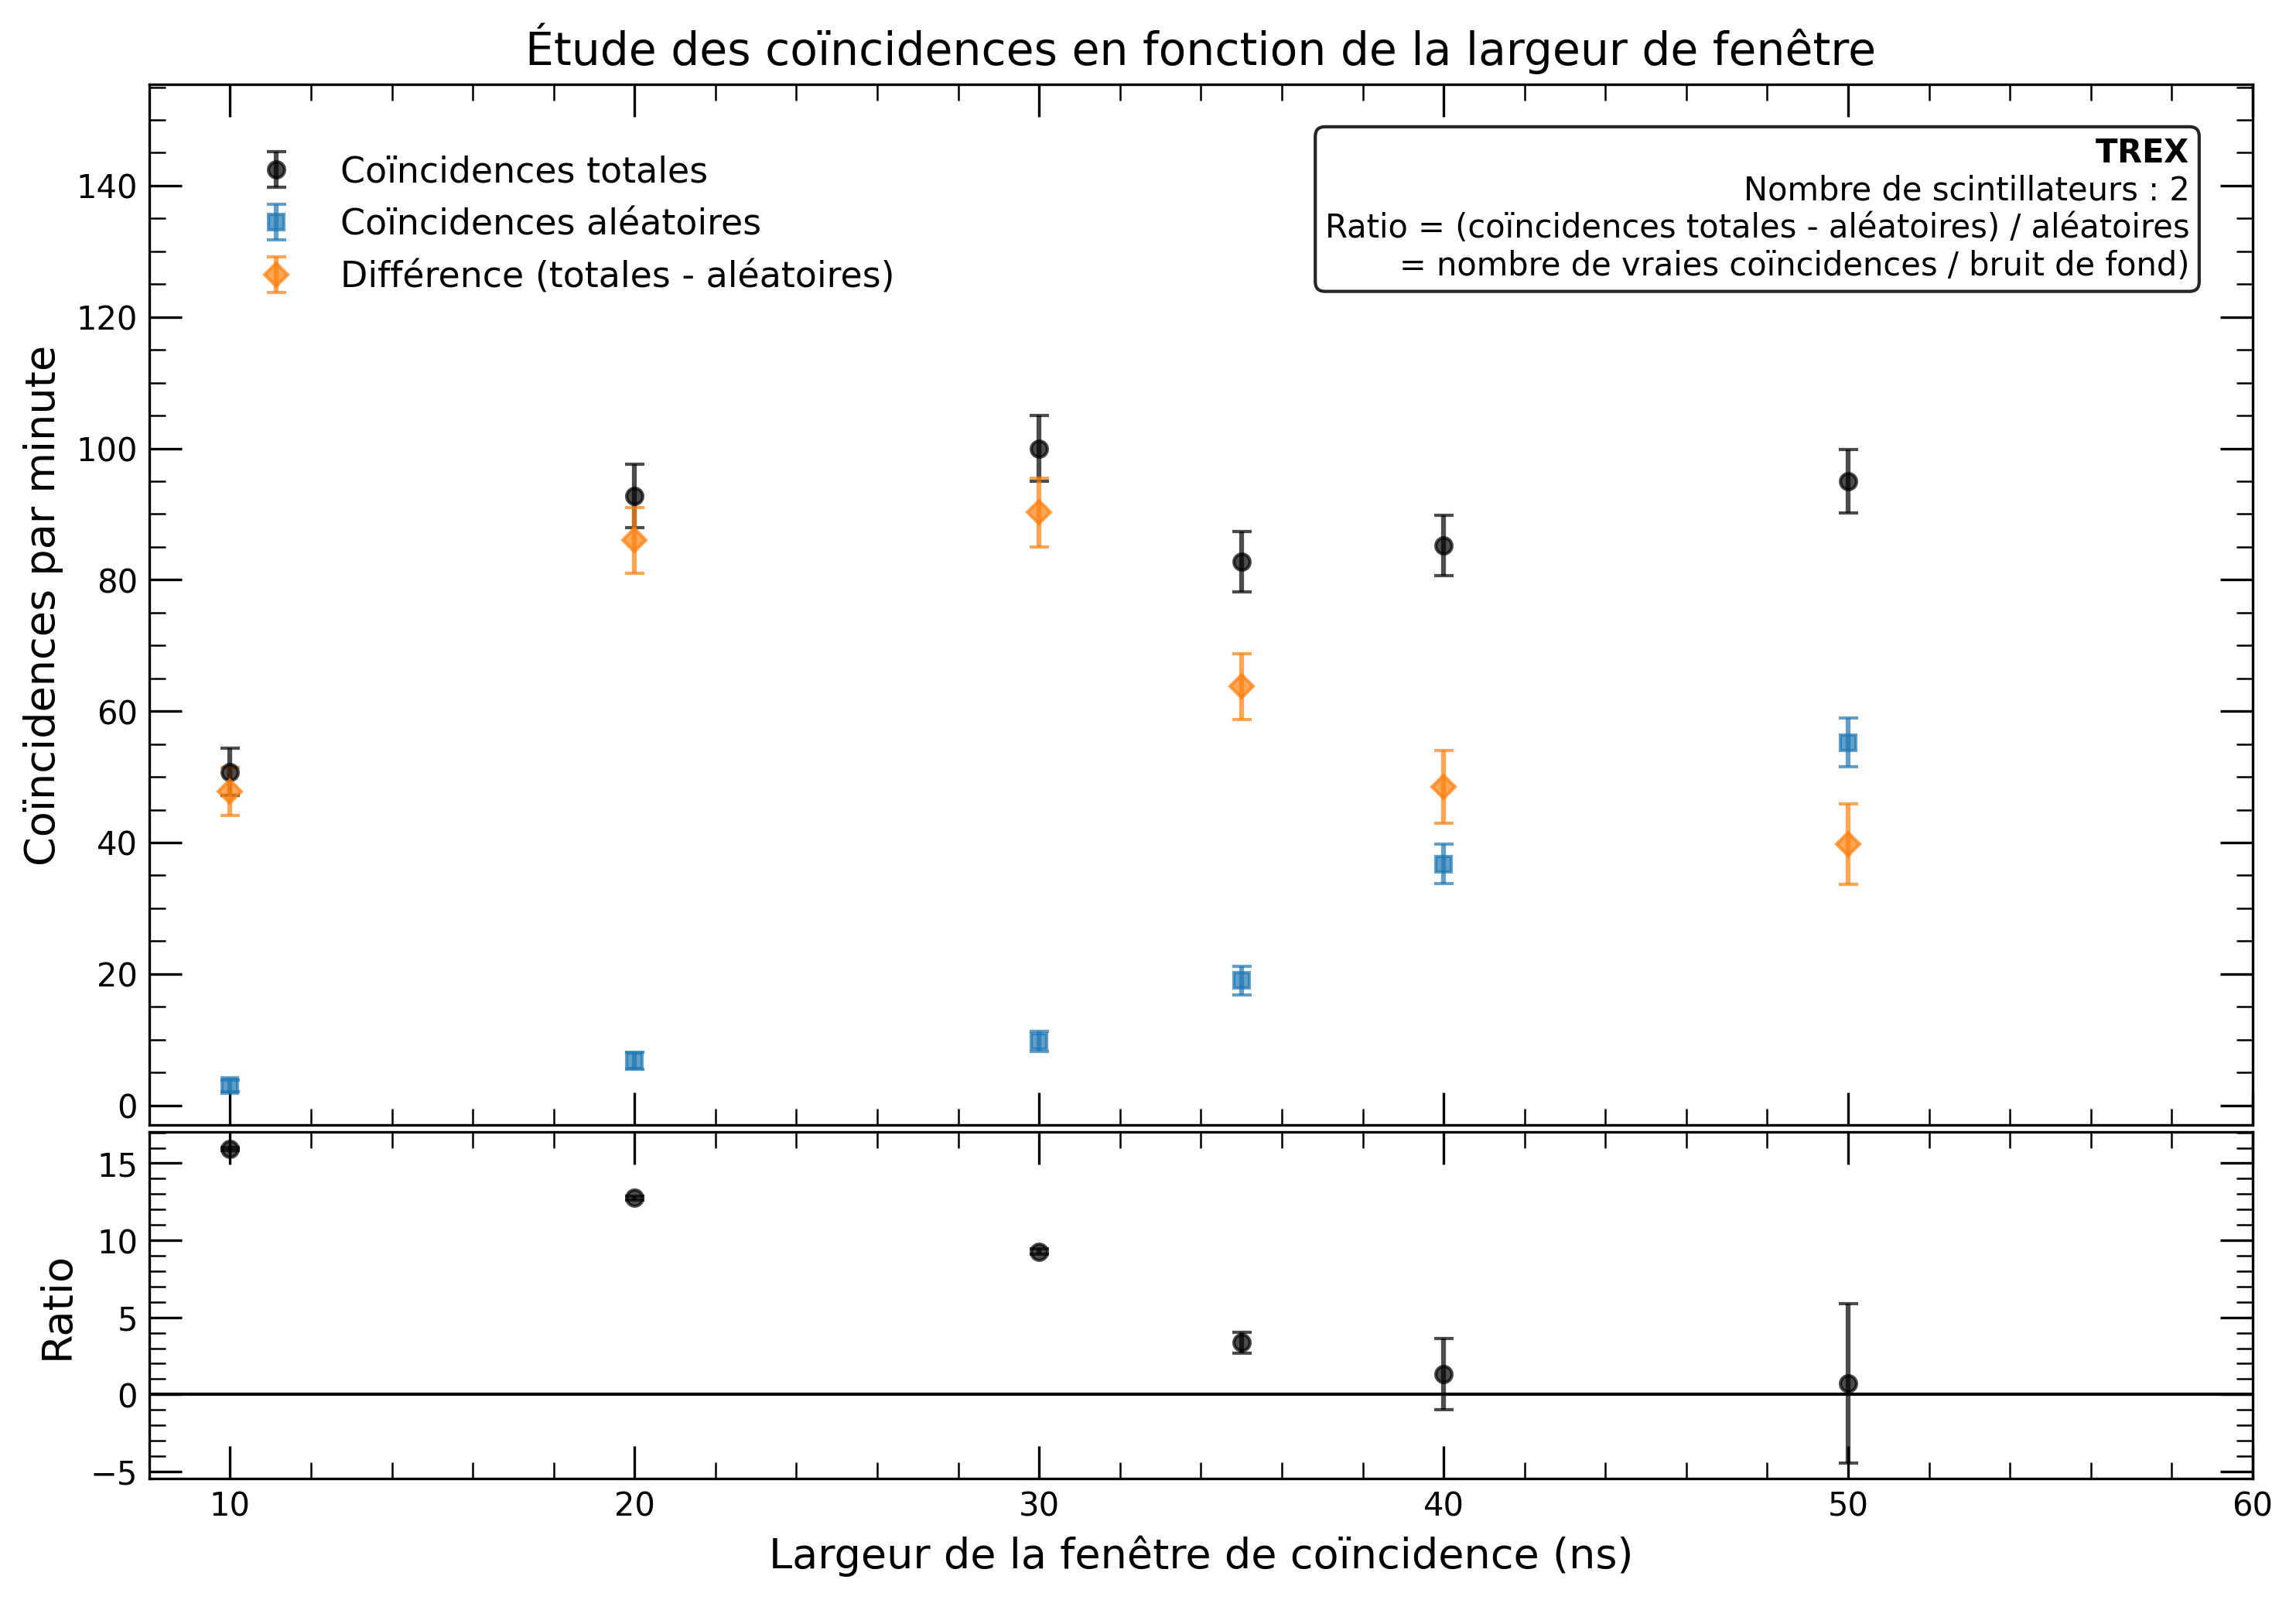
\includegraphics[width=0.8\textwidth]{Images/Coincidences_2_Scintillateurs.png}
    \caption[Nombre d’évènement en 4 min en fonction du seuil]{Nombre d’évènement en 4min en fonction du seuil pour 2 scintillateurs en coïncidence.
    On voit que le nombre de coïncidences fortuites augmente fortement avec la largeur de fenêtre, tandis que le nombre de vrais muons détectés reste relativement stable et forme un palier au valeures de width optimales.}
    \label{fig:coincidences_2_scintillateurs}
\end{figure}

\newpage

\subsubsection{Coïncidence à 3 scintillateurs}

Le graphique ci-dessous (figure \ref{fig:coincidences_3_scintillateurs}) présente les résultats obtenus pour la coïncidence à 3 scintillateurs, avec les réglages suivants :
\begin{itemize}
    \item Scintillateur 1 : seuil de 0{,}45~V, haute tension de 2000~V
    \item Scintillateur 2 : seuil de 0{,}05~V, haute tension de 2050~V, delay = 63~ns
    \item Scintillateur 3 : seuil de 0{,}3~V, haute tension de 2060~V, delay = 31~ns
\end{itemize}
Ces valeurs ont été choisies à partir des optimisations précédentes.

Pour chaque largeur de fenêtre de coïncidence (width), on a mesuré :
\begin{itemize}
    \item le nombre total de coïncidences enregistrées en 10 minute (sans délai)~;
    \item le nombre de coïncidences fortuites (avec deux délais différents)~;
    \item la différence entre les deux, qui correspond au nombre de “vrais” muons détectés~;
    \item le ratio entre le nombre de vraies coïncidences et le nombre de coïncidences fortuites, indicateur direct de la pureté du signal.
\end{itemize}

On constate que l’utilisation de trois scintillateurs permet de réduire le nombre de coïncidences fortuites, et que le ratio signal/bruit devient plus élevé. Ce protocole permet donc d’obtenir un signal muonique pur, au prix d’un nombre d’événements plus faible.

\begin{figure}[H]
    \centering
    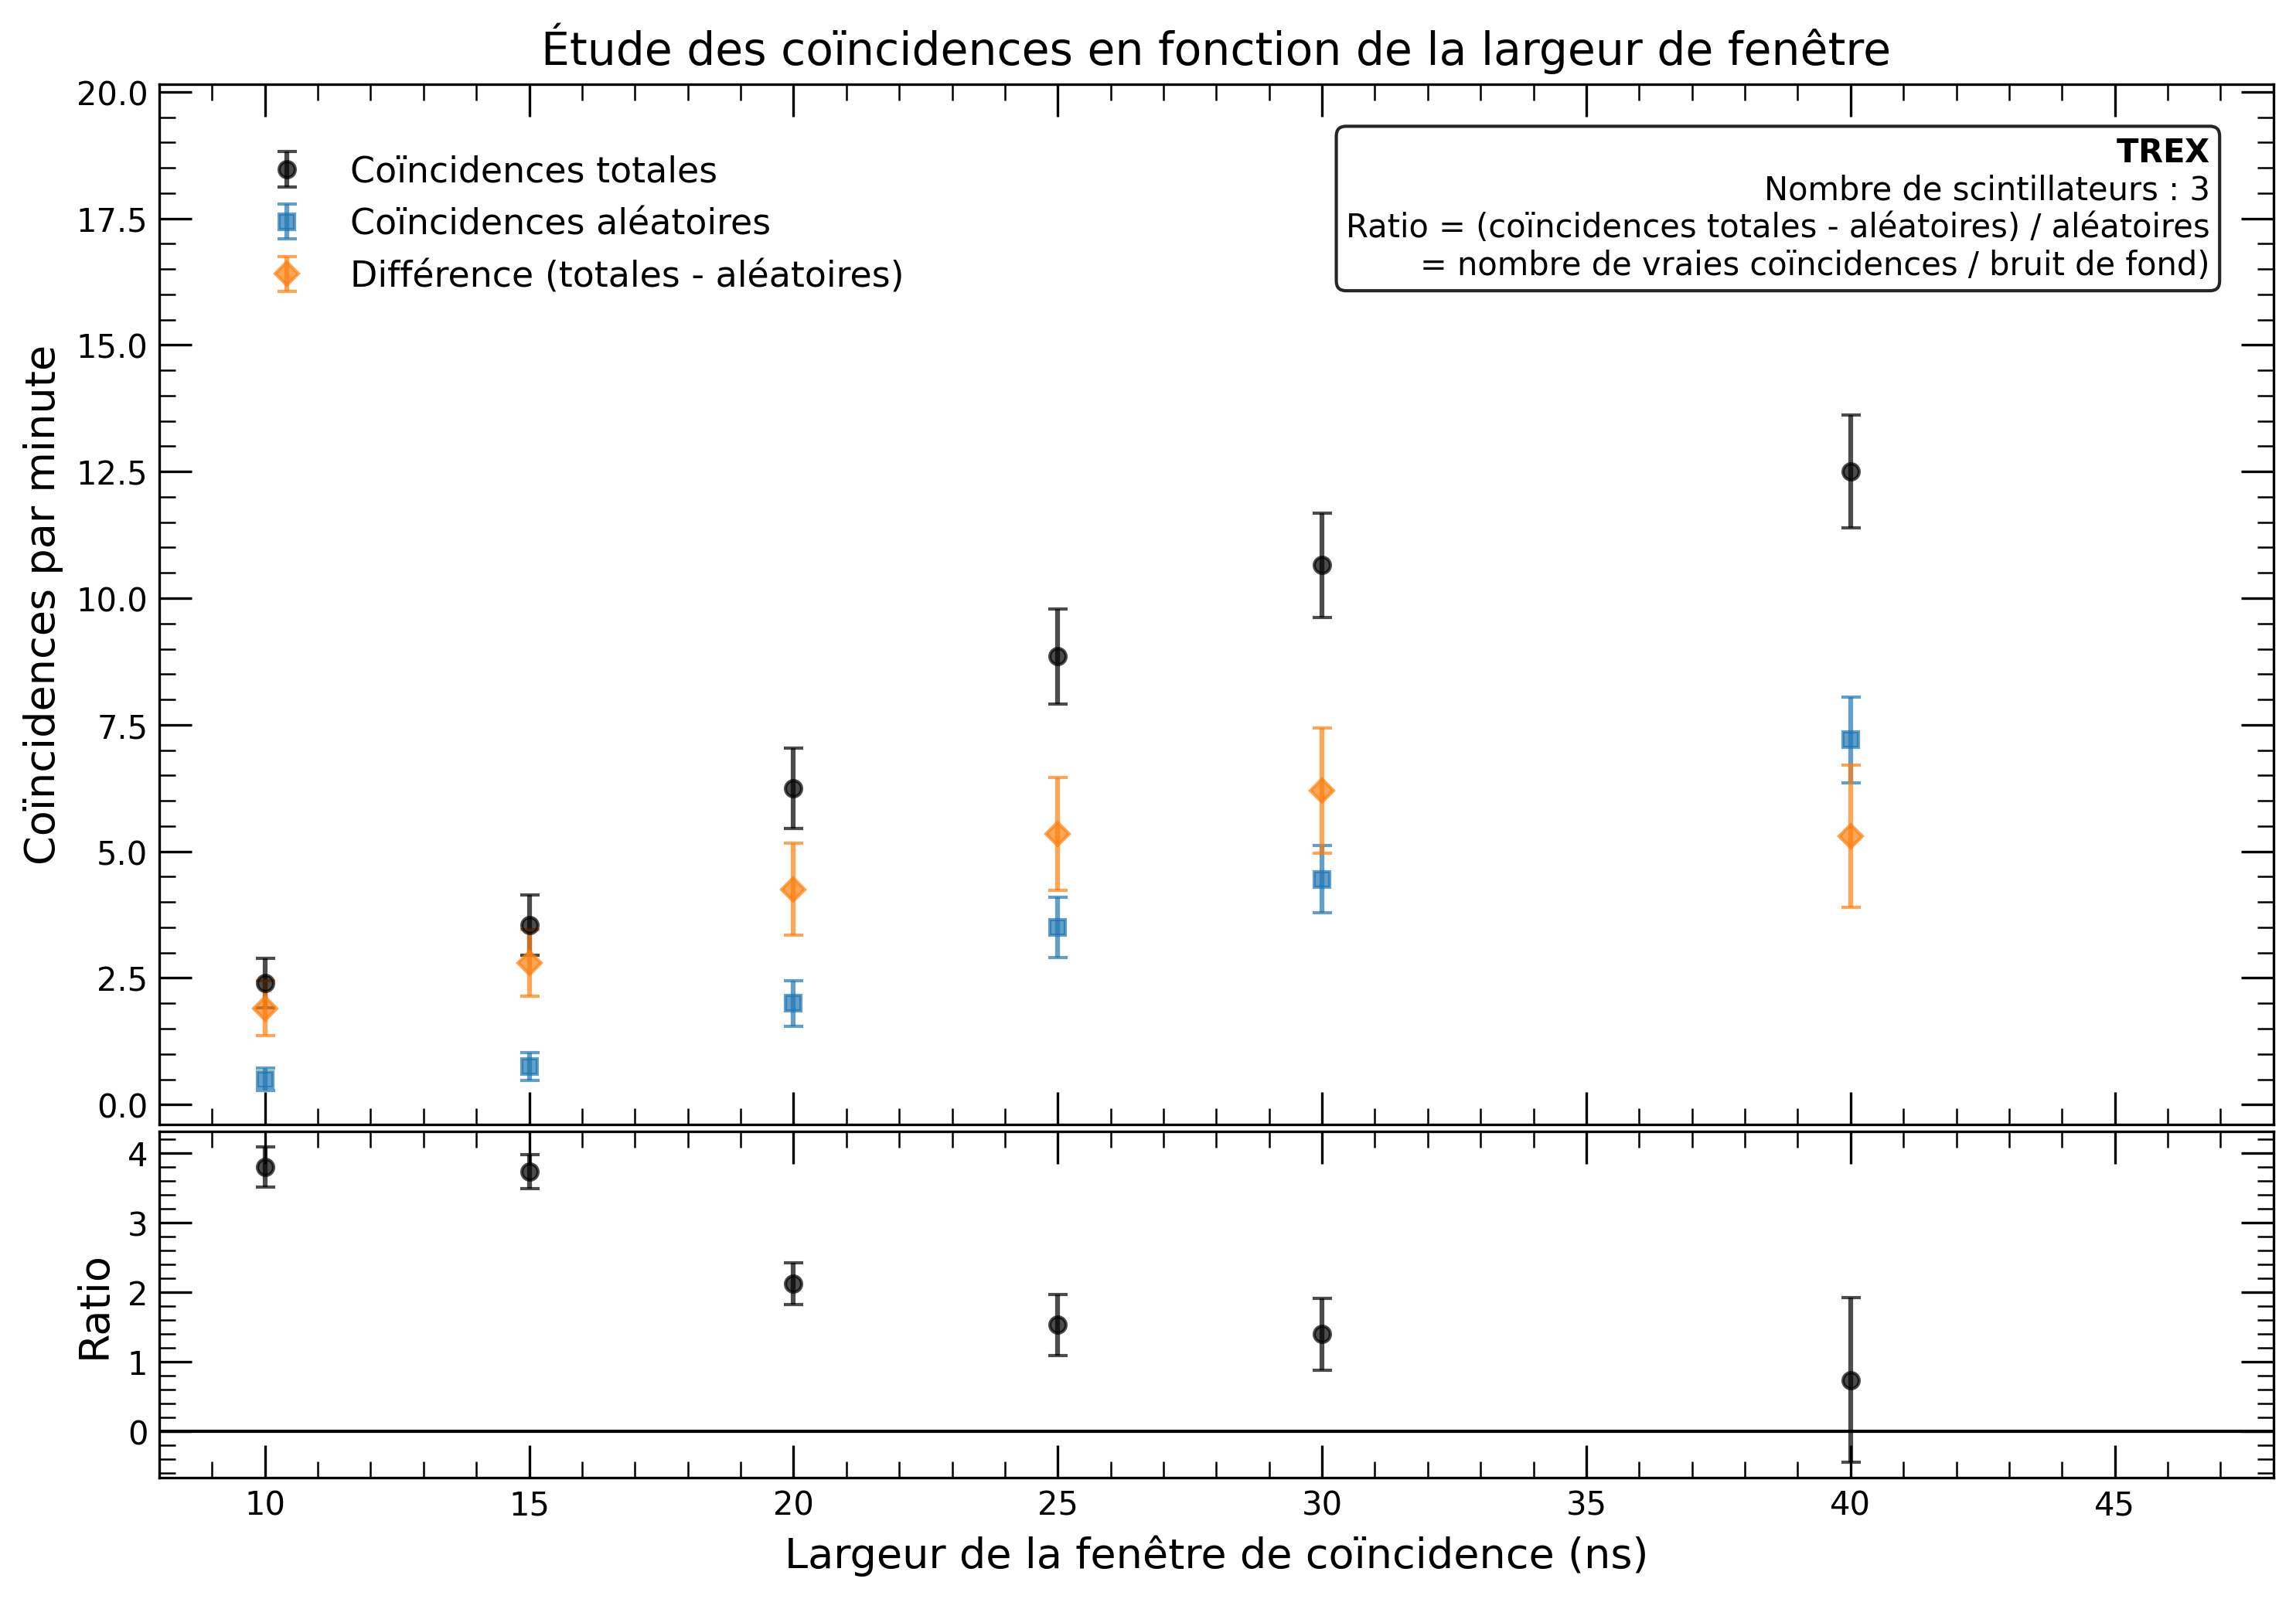
\includegraphics[width=0.8\textwidth]{Images/Coincidences_3_Scintillateurs.png}
    \caption[Nombre d’évènement en 4min en fonction du seuil]{Nombre d’évènement en 10 min en fonction du seuil pour 3 scintillateurs en coïncidence.
    Le choix de la width optimale est crucial pour maximiser le nombre de vrais muons détectés tout en minimisant le bruit de fond. On observe que pour une width de 20 ns, le taux de coïncidences fortuites est faible tout en ayant un nombre de coïncidences raisonnable, ce qui permet d’obtenir un signal muonique sensiblement pur.}
    \label{fig:coincidences_3_scintillateurs}
  \end{figure}

% --- Encadré Problèmes rencontrés lors des mesures de coïncidences ---

\begin{center}
\begin{tcolorbox}[colback=red!5!white, colframe=red!80!black, title=Problèmes rencontrés lors des mesures de coïncidences]
Lors des mesures de coïncidences (notamment à 3 scintillateurs), plusieurs difficultés majeures ont été rencontrées :
\begin{itemize}
    \item \textbf{Nombre de coïncidences très faible} : surtout avec 3 scintillateurs, le taux de coïncidences était très bas, nécessitant des temps d'acquisition très longs (parfois 10 minutes par point), ce qui a rendu les manipulations longues et sujettes à de grandes incertitudes statistiques.
    \item \textbf{Différences entre scintillateurs} : le nombre de coïncidences à 2 scintillateurs dépendait fortement de la paire choisie, les scintillateurs étant très différents en efficacité. De nombreux tests ont été nécessaires pour choisir la meilleure combinaison.
    \item \textbf{Retard dans les câbles} : le retard dû à la longueur des câbles diffère selon le scintillateur. Nous avons supposé cet effet négligeable, mais il a pu influencer les mesures.
    \item \textbf{Ratio signal/bruit inattendu} : on s’attendait à ce que le ratio (nombre de vrais muons détectés divisé par le nombre de fausses coïncidences) soit plus grand pour 3 scintillateurs que pour 2, mais nous avons observé l’inverse. Cela peut s’expliquer par le très faible nombre de détections, malgré un temps d’acquisition de 10 minutes, ce qui augmente l’incertitude statistique et peut fausser le ratio mesuré. Il est aussi possible qu’une défaillance ou une usure d'un des scintillateurs ait fortement réduit la zone de détection réelle (plus petite que la surface du scintillateur), ce qui diminue le nombre de “vrais” muons détectés. À noter que pour les mesures à 2 scintillateurs, nous avions sélectionné les deux détecteurs les plus efficaces, ce qui a permis d’obtenir de meilleures données.
\end{itemize}
Ces limitations ont rendu l’optimisation fine difficile et expliquent la dispersion des résultats.
\end{tcolorbox}
\end{center}

% --- Synthèse résultats coïncidences ---

\begin{remarque}
\textbf{Synthèse~:} Pour la coïncidence à 2 scintillateurs, la largeur de fenêtre optimale retenue est de \textbf{20 ns}, ce qui permet d’obtenir un taux de coïncidences fortuites inférieur à \textbf{10\%} du total. Pour 3 scintillateurs, une fenêtre de \textbf{20 ns} rend le taux de coïncidences fortuites faible tout en ayant un nombre de coïncidences raisonnable.

Ces résultats étaient censés montrer que l’ajout d’un troisième scintillateur permet d’obtenir un signal muonique plus pur, au prix d’un nombre d’événements plus faible. Le réglage fin de la fenêtre de coïncidence est donc crucial pour maximiser la pureté du signal tout en conservant une statistique exploitable.
\end{remarque}

\newpage

\section{Distribution angulaire du flux muonique}
L'un des caract\`eres notables du rayonnement cosmique muonique au niveau du sol est son anisotropie en angle \text{\'enithal}. Les muons proviennent majoritairement de la verticale, c'est-\`a-dire de la direction du \text{\'enith} (car ils sont g\'en\'er\'es en haute atmosph\`ere et suivent grossi\`erement des trajectoires quasi-rectilignes vers le bas). Plus l'angle~$\theta$ par rapport \`a la verticale augmente (muons venant rasants de l'horizon), plus le parcours dans l'atmosph\`ere est long, et donc plus la probabilit\'e de survie du muon jusqu'au sol diminue. Ce ph\'enom\`ene se traduit par une loi empirique proche de
\[
  I(\theta) = I(0)\cos^n\theta,
\]
avec $n \approx 2$ aux 'energies cosmiques typiques. Autrement dit, le flux diff\'erentiel de muons est approximativement proportionnel \`a $\cos^2\theta$ pour des angles mod\'er\'es. Des mesures plus fines montrent qu'\`a tr\`es grands angles ($\theta > 60^\circ$), la distribution s'att\'enue plus fortement que le simple $\cos^2$ en raison de la courbure terrestre (au-del\`a d'un certain angle, les muons provenant de l'horizon ont parcouru une distance atmosph\`erique si grande qu'aucun n'atteint le sol) et de la s\'election en 'energie (seuls les muons les plus 'energiques arrivent depuis des angles rasants sans se d\'esint\'egrer). N\'eanmoins, dans l'intervalle $0^\circ \le \theta \leq 60^\circ$, on peut consid\'erer la loi $\cos^2\theta$ comme une bonne approximation pour le flux muonique au niveau de la mer.

\subsection{Mise en œuvre expérimentale}

\begin{figure}[H]
  \begin{minipage}{0.3\textwidth}
    \centering
    

\tikzset{every picture/.style={line width=0.75pt}} %set default line width to 0.75pt        

\begin{tikzpicture}[x=0.75pt,y=0.75pt,yscale=-1,xscale=1]
%uncomment if require: \path (0,300); %set diagram left start at 0, and has height of 300

%Straight Lines [id:da10698561364234205] 
\draw [line width=1.5]    (119,200) -- (221,200) ;
\draw [shift={(217,200)}, rotate = 0] [fill={rgb, 255:red, 0; green, 0; blue, 0 }  ][line width=0.08]  [draw opacity=0] (15.6,-3.9) -- (0,0) -- (15.6,3.9) -- cycle    ;
\draw [shift={(123,200)}, rotate = 180] [fill={rgb, 255:red, 0; green, 0; blue, 0 }  ][line width=0.08]  [draw opacity=0] (15.6,-3.9) -- (0,0) -- (15.6,3.9) -- cycle    ;
%Straight Lines [id:da33060194224587247] 
\draw [line width=1.5]    (119,150) -- (221,150) ;
\draw [shift={(217,150)}, rotate = 0] [fill={rgb, 255:red, 0; green, 0; blue, 0 }  ][line width=0.08]  [draw opacity=0] (15.6,-3.9) -- (0,0) -- (15.6,3.9) -- cycle    ;
\draw [shift={(123,150)}, rotate = 180] [fill={rgb, 255:red, 0; green, 0; blue, 0 }  ][line width=0.08]  [draw opacity=0] (15.6,-3.9) -- (0,0) -- (15.6,3.9) -- cycle    ;
%Straight Lines [id:da8560408409642792] 
\draw [line width=1.5]    (119,100) -- (221,100) ;
\draw [shift={(217,100)}, rotate = 0] [fill={rgb, 255:red, 0; green, 0; blue, 0 }  ][line width=0.08]  [draw opacity=0] (15.6,-3.9) -- (0,0) -- (15.6,3.9) -- cycle    ;
\draw [shift={(123,100)}, rotate = 180] [fill={rgb, 255:red, 0; green, 0; blue, 0 }  ][line width=0.08]  [draw opacity=0] (15.6,-3.9) -- (0,0) -- (15.6,3.9) -- cycle    ;
%Straight Lines [id:da9600498294764344] 
\draw [color={rgb, 255:red, 208; green, 2; blue, 27 }  ,draw opacity=1 ]   (170,40) -- (170,220) ;
\draw [shift={(170,140)}, rotate = 270] [color={rgb, 255:red, 208; green, 2; blue, 27 }  ,draw opacity=1 ][line width=0.75]    (17.64,-3.29) .. controls (13.66,-1.4) and (10.02,-0.3) .. (6.71,0) .. controls (10.02,0.3) and (13.66,1.4) .. (17.64,3.29)(10.93,-3.29) .. controls (6.95,-1.4) and (3.31,-0.3) .. (0,0) .. controls (3.31,0.3) and (6.95,1.4) .. (10.93,3.29)   ;
%Straight Lines [id:da775185348030494] 
\draw [color={rgb, 255:red, 208; green, 2; blue, 27 }  ,draw opacity=1 ]   (210,40) -- (210,220) ;
\draw [shift={(210,140)}, rotate = 270] [color={rgb, 255:red, 208; green, 2; blue, 27 }  ,draw opacity=1 ][line width=0.75]    (17.64,-3.29) .. controls (13.66,-1.4) and (10.02,-0.3) .. (6.71,0) .. controls (10.02,0.3) and (13.66,1.4) .. (17.64,3.29)(10.93,-3.29) .. controls (6.95,-1.4) and (3.31,-0.3) .. (0,0) .. controls (3.31,0.3) and (6.95,1.4) .. (10.93,3.29)   ;
%Straight Lines [id:da37087677634539107] 
\draw [color={rgb, 255:red, 208; green, 2; blue, 27 }  ,draw opacity=1 ]   (130,40) -- (130,220) ;
\draw [shift={(130,140)}, rotate = 270] [color={rgb, 255:red, 208; green, 2; blue, 27 }  ,draw opacity=1 ][line width=0.75]    (17.64,-3.29) .. controls (13.66,-1.4) and (10.02,-0.3) .. (6.71,0) .. controls (10.02,0.3) and (13.66,1.4) .. (17.64,3.29)(10.93,-3.29) .. controls (6.95,-1.4) and (3.31,-0.3) .. (0,0) .. controls (3.31,0.3) and (6.95,1.4) .. (10.93,3.29)   ;




\end{tikzpicture}

    \caption{Montage de mesure de l'angle nul.\\Les trois scintillateurs sont alignés, comme depuis le début du TREX.}
    \label{fig:angle_nul}
  \end{minipage}
  \hfill
  \begin{minipage}
  {0.3\textwidth}
    \centering
    

\tikzset{every picture/.style={line width=0.75pt}} %set default line width to 0.75pt        

\begin{tikzpicture}[x=0.75pt,y=0.75pt,yscale=-1,xscale=1]
%uncomment if require: \path (0,300); %set diagram left start at 0, and has height of 300

%Straight Lines [id:da3640087483511575] 
\draw [line width=1.5]    (249,200) -- (351,200) ;
\draw [shift={(347,200)}, rotate = 0] [fill={rgb, 255:red, 0; green, 0; blue, 0 }  ][line width=0.08]  [draw opacity=0] (15.6,-3.9) -- (0,0) -- (15.6,3.9) -- cycle    ;
\draw [shift={(253,200)}, rotate = 180] [fill={rgb, 255:red, 0; green, 0; blue, 0 }  ][line width=0.08]  [draw opacity=0] (15.6,-3.9) -- (0,0) -- (15.6,3.9) -- cycle    ;
%Straight Lines [id:da3186253744227674] 
\draw [line width=1.5]    (279,150) -- (381,150) ;
\draw [shift={(377,150)}, rotate = 0] [fill={rgb, 255:red, 0; green, 0; blue, 0 }  ][line width=0.08]  [draw opacity=0] (15.6,-3.9) -- (0,0) -- (15.6,3.9) -- cycle    ;
\draw [shift={(283,150)}, rotate = 180] [fill={rgb, 255:red, 0; green, 0; blue, 0 }  ][line width=0.08]  [draw opacity=0] (15.6,-3.9) -- (0,0) -- (15.6,3.9) -- cycle    ;
%Straight Lines [id:da7715340597742683] 
\draw [line width=1.5]    (309,100) -- (411,100) ;
\draw [shift={(407,100)}, rotate = 0] [fill={rgb, 255:red, 0; green, 0; blue, 0 }  ][line width=0.08]  [draw opacity=0] (15.6,-3.9) -- (0,0) -- (15.6,3.9) -- cycle    ;
\draw [shift={(313,100)}, rotate = 180] [fill={rgb, 255:red, 0; green, 0; blue, 0 }  ][line width=0.08]  [draw opacity=0] (15.6,-3.9) -- (0,0) -- (15.6,3.9) -- cycle    ;
%Straight Lines [id:da2209761946060118] 
\draw [color={rgb, 255:red, 208; green, 2; blue, 27 }  ,draw opacity=1 ]   (390,40) -- (290,220) ;
\draw [shift={(335.14,138.74)}, rotate = 299.05] [color={rgb, 255:red, 208; green, 2; blue, 27 }  ,draw opacity=1 ][line width=0.75]    (17.64,-3.29) .. controls (13.66,-1.4) and (10.02,-0.3) .. (6.71,0) .. controls (10.02,0.3) and (13.66,1.4) .. (17.64,3.29)(10.93,-3.29) .. controls (6.95,-1.4) and (3.31,-0.3) .. (0,0) .. controls (3.31,0.3) and (6.95,1.4) .. (10.93,3.29)   ;
%Straight Lines [id:da18669424338790397] 
\draw [color={rgb, 255:red, 208; green, 2; blue, 27 }  ,draw opacity=1 ]   (430,40) -- (330,220) ;
\draw [shift={(375.14,138.74)}, rotate = 299.05] [color={rgb, 255:red, 208; green, 2; blue, 27 }  ,draw opacity=1 ][line width=0.75]    (17.64,-3.29) .. controls (13.66,-1.4) and (10.02,-0.3) .. (6.71,0) .. controls (10.02,0.3) and (13.66,1.4) .. (17.64,3.29)(10.93,-3.29) .. controls (6.95,-1.4) and (3.31,-0.3) .. (0,0) .. controls (3.31,0.3) and (6.95,1.4) .. (10.93,3.29)   ;
%Straight Lines [id:da20749689744180777] 
\draw [color={rgb, 255:red, 208; green, 2; blue, 27 }  ,draw opacity=1 ]   (350,40) -- (250,220) ;
\draw [shift={(295.14,138.74)}, rotate = 299.05] [color={rgb, 255:red, 208; green, 2; blue, 27 }  ,draw opacity=1 ][line width=0.75]    (17.64,-3.29) .. controls (13.66,-1.4) and (10.02,-0.3) .. (6.71,0) .. controls (10.02,0.3) and (13.66,1.4) .. (17.64,3.29)(10.93,-3.29) .. controls (6.95,-1.4) and (3.31,-0.3) .. (0,0) .. controls (3.31,0.3) and (6.95,1.4) .. (10.93,3.29)   ;




\end{tikzpicture}

    \caption{Montage de mesure pour un angle non nul.\\Les trois scintillateurs sont déplacés horizontalement pour sélectionner les muons incidents.}
    \label{fig:angle_non_nul}
  \end{minipage}
  \hfill
  \begin{minipage}{0.3\textwidth}
    \centering
    

\tikzset{every picture/.style={line width=0.75pt}} %set default line width to 0.75pt        

\begin{tikzpicture}[x=0.75pt,y=0.75pt,yscale=-1,xscale=1]
%uncomment if require: \path (0,300); %set diagram left start at 0, and has height of 300

%Straight Lines [id:da7299563947294572] 
\draw [line width=1.5]    (409,200) -- (511,200) ;
\draw [shift={(507,200)}, rotate = 0] [fill={rgb, 255:red, 0; green, 0; blue, 0 }  ][line width=0.08]  [draw opacity=0] (15.6,-3.9) -- (0,0) -- (15.6,3.9) -- cycle    ;
\draw [shift={(413,200)}, rotate = 180] [fill={rgb, 255:red, 0; green, 0; blue, 0 }  ][line width=0.08]  [draw opacity=0] (15.6,-3.9) -- (0,0) -- (15.6,3.9) -- cycle    ;
%Straight Lines [id:da15545310486444974] 
\draw [line width=1.5]    (439,150) -- (541,150) ;
\draw [shift={(537,150)}, rotate = 0] [fill={rgb, 255:red, 0; green, 0; blue, 0 }  ][line width=0.08]  [draw opacity=0] (15.6,-3.9) -- (0,0) -- (15.6,3.9) -- cycle    ;
\draw [shift={(443,150)}, rotate = 180] [fill={rgb, 255:red, 0; green, 0; blue, 0 }  ][line width=0.08]  [draw opacity=0] (15.6,-3.9) -- (0,0) -- (15.6,3.9) -- cycle    ;
%Straight Lines [id:da6023595366311324] 
\draw [line width=1.5]    (469,100) -- (571,100) ;
\draw [shift={(567,100)}, rotate = 0] [fill={rgb, 255:red, 0; green, 0; blue, 0 }  ][line width=0.08]  [draw opacity=0] (15.6,-3.9) -- (0,0) -- (15.6,3.9) -- cycle    ;
\draw [shift={(473,100)}, rotate = 180] [fill={rgb, 255:red, 0; green, 0; blue, 0 }  ][line width=0.08]  [draw opacity=0] (15.6,-3.9) -- (0,0) -- (15.6,3.9) -- cycle    ;
%Straight Lines [id:da6024888939047257] 
\draw [color={rgb, 255:red, 208; green, 2; blue, 27 }  ,draw opacity=1 ]   (510,40) -- (410,220) ;
\draw [shift={(455.14,138.74)}, rotate = 299.05] [color={rgb, 255:red, 208; green, 2; blue, 27 }  ,draw opacity=1 ][line width=0.75]    (17.64,-3.29) .. controls (13.66,-1.4) and (10.02,-0.3) .. (6.71,0) .. controls (10.02,0.3) and (13.66,1.4) .. (17.64,3.29)(10.93,-3.29) .. controls (6.95,-1.4) and (3.31,-0.3) .. (0,0) .. controls (3.31,0.3) and (6.95,1.4) .. (10.93,3.29)   ;
%Straight Lines [id:da19930734627499203] 
\draw [color={rgb, 255:red, 126; green, 211; blue, 33 }  ,draw opacity=1 ]   (460,40) -- (510,220) ;
\draw [shift={(487.68,139.64)}, rotate = 254.48] [color={rgb, 255:red, 126; green, 211; blue, 33 }  ,draw opacity=1 ][line width=0.75]    (17.64,-3.29) .. controls (13.66,-1.4) and (10.02,-0.3) .. (6.71,0) .. controls (10.02,0.3) and (13.66,1.4) .. (17.64,3.29)(10.93,-3.29) .. controls (6.95,-1.4) and (3.31,-0.3) .. (0,0) .. controls (3.31,0.3) and (6.95,1.4) .. (10.93,3.29)   ;
%Straight Lines [id:da7853228122624806] 
\draw [color={rgb, 255:red, 74; green, 144; blue, 226 }  ,draw opacity=1 ]   (590,40) -- (410,220) ;
\draw [shift={(492.93,137.07)}, rotate = 315] [color={rgb, 255:red, 74; green, 144; blue, 226 }  ,draw opacity=1 ][line width=0.75]    (17.64,-3.29) .. controls (13.66,-1.4) and (10.02,-0.3) .. (6.71,0) .. controls (10.02,0.3) and (13.66,1.4) .. (17.64,3.29)(10.93,-3.29) .. controls (6.95,-1.4) and (3.31,-0.3) .. (0,0) .. controls (3.31,0.3) and (6.95,1.4) .. (10.93,3.29)   ;




\end{tikzpicture}

    \caption{Effet de la largeur des scintillateurs sur la pureté angulaire. On voit que la largeur réelle des scintillateurs ne permet pas une sélection très pure des angles.}
    \label{fig:range_des_angles}
  \end{minipage}
  \caption{Montages expérimentaux pour la mesure angulaire des muons.}
\end{figure}


\begin{center}
\begin{tcolorbox}[colback=blue!5!white, colframe=blue!60!black, title=Principe de la sélection angulaire par déplacement des scintillateurs]
En pratique, une première idée consiste à faire varier l’angle d’incidence des muons en déplaçant horizontalement les scintillateurs.
 Les muons sont alors sélectionnés selon leur angle d’incidence, comme schématisé en figure~\ref{fig:angle_non_nul}.
 
\end{tcolorbox}
\end{center}
Cependant, la mesure est tres imprecise car la sélection des angles est très impûre comme on peu le comprendre grace a la figure \ref{fig:range_des_angles}.
En effet, la largeur des scintillateurs est de l'ordre de 20cm ce qui fait que la sélection des angles est tres large.
Une fois les scintillateurs correctements placés, pour chaque angle~$\theta$, on enregistre le nombre de muons détectés (coïncidences $A\wedge B\wedge C$) pendant une durée fixe. On obtient ainsi un taux de comptage~$N(\theta)$ en fonction de~$\theta$. Les résultats bruts doivent être corrigés d'un effet géométrique~: la projection de la surface du détecteur selon l'angle. Lorsque les scintillateurs sont deplacés la surface effective presenté au muons venant avec un angle d'incidence $\theta$, est réduite d'un facteur~$\cos\theta$. 

Après ces corrections, on peut comparer la distribution normalisée~$I_{\mathrm{mesure}}(\theta)$ au modèle en~$\cos^{2}\theta$. Les données obtenues présentent une bonne conformité avec la loi attendue. 
Figure \ref{fig:cos2s} ci‑dessous montre, de façon qualitative, la tendance mesurée~: en représentant $N(\theta)$ corrigé en fonction de~$\cos\theta$, on obtient approximativement une droite, ce qui traduit
\[
N(\theta)\propto\cos^{2}\theta.
\]
\begin{figure}[!h]
  \centering
  \includegraphics[width=0.7\textwidth]{Images/coscarréavectroisscintillateurs.png}
  \caption{Flux de muons mesuré en fonction de l'angle d'incidence $\theta$. On observe une décroissance du flux avec l'angle, confirmant la loi $\cos^2\theta$. On note l'imprecision de la mesure du au conditions experimentales.}
  \label{fig:cos2s}
\end{figure}

\textbf{Interprétation}~: la loi $I(\theta)\propto\cos^2\theta$ résulte de la combinaison de deux effets principaux.  
(i) Distribution isotrope à la production~: les pions parents des muons sont produits isotropiquement dans le référentiel du laboratoire (en première approximation), et leur désintégration donne des muons distribués également dans l'espace (avec un léger biais avant, négligeable ici).
Ainsi, le flux de muons incident sur la Terre en l'absence d'atmosphère serait isotrope, donc $\propto\cos\theta$ simplement à cause de la projection de surface.  
(ii) Parcours atmosphérique variable~: les muons créés à un angle~$\theta$ doivent traverser une épaisseur d'atmosphère $X(\theta)$ plus grande que ceux venant du zénith. Pour un angle zénithal~$\theta$, la longueur parcourue est approximativement
\[
L(\theta)=\frac{L(0)}{\cos\theta}
\]
(pour $\theta$ pas trop grand et en négligeant la courbure terrestre), où $L(0)$ est l'épaisseur de l'atmosphère. La probabilité de survie d'un muon jusqu'au sol décroît exponentiellement avec~$L$:
\[
P_{\mathrm{survie}}(\theta)\approx\exp\bigl(-L(\theta)/\Lambda_{\mu}\bigr),
\]
avec $\Lambda_{\mu}$ la longueur d'atténuation (liée à la longueur de désintégration $\gamma c\tau$ des muons, de l'ordre de~6 km d'équivalent air pour des muons de quelques GeV):
\[
P(\theta)\approx \exp\!\Bigl(-\tfrac{L(0)}{\Lambda_\mu}\tfrac1{\cos\theta}\Bigr)
\]
Si $\tfrac{L(0)}{\Lambda_\mu}$ n'est pas trop grand (typiquement 1--3), on peut approximer pour des petits angles~$\theta$:
\[
\exp\!\Bigl(-\tfrac1{\cos\theta}\tfrac{X(0)}{\Lambda_\mu}\Bigr)\sim\cos^n\theta
\]
pour un certain~$n$. Les valeurs réalistes donnent effectivement un $n\approx2$. En réalité, le spectre en énergie entre aussi en jeu : les muons plus inclinés doivent avoir une énergie plus grande pour survivre (sinon ils se désintègrent en route), ce qui modifie légèrement l'exposant~$n$ en fonction du seuil d'énergie considéré. Néanmoins, dans l'intervalle $0^\circ \le \theta \leq 60^\circ$, on peut consid\'erer la loi $\cos^2\theta$ comme une bonne approximation pour le flux muonique au niveau de la mer.

\begin{center}
\begin{tcolorbox}[colback=red!5!white, colframe=red!80!black, title=Limites et problèmes de la sélection angulaire par déplacement des scintillateurs]
Cette méthode présente plusieurs limitations expérimentales :
\begin{itemize}
    \item \textbf{Sélection angulaire imprécise~:} La largeur importante des scintillateurs (environ 20~cm) fait que chaque configuration sélectionne en réalité une large gamme d’angles, ce qui réduit la pureté directionnelle de la mesure (voir figure~\ref{fig:range_des_angles}).
    \item \textbf{Effet géométrique~:} La surface effective du détecteur diminue avec l’angle, ce qui nécessite une correction par un facteur $\cos\theta$ pour comparer les taux de comptage.
    \item \textbf{Statistique limitée~:} Pour les grands angles, le flux de muons détectés devient faible, ce qui augmente l’incertitude statistique.
    \item \textbf{Alignement et reproductibilité~:} Le repositionnement manuel des scintillateurs peut introduire des erreurs d’alignement et de reproductibilité d’une mesure à l’autre.
    \item \textbf{Homogeneité des scintillateurs~:} Les différentes zones d'impact des muons peut introduire des biais si les scintillateurs ne sont pas parfaitement homogènes en efficacité de détection.
  \end{itemize}
Ces limitations expliquent la dispersion des résultats (si on arrive à mettre en évidence une tendance, la modelisation des données est assez aproximative.) et motivent l’utilisation de dispositifs plus performants, comme la matrice de scintillateurs.
\end{tcolorbox}
\end{center}


\subsection{Deuxième méthode de mesure}


\begin{figure}[!h]
  \centering
  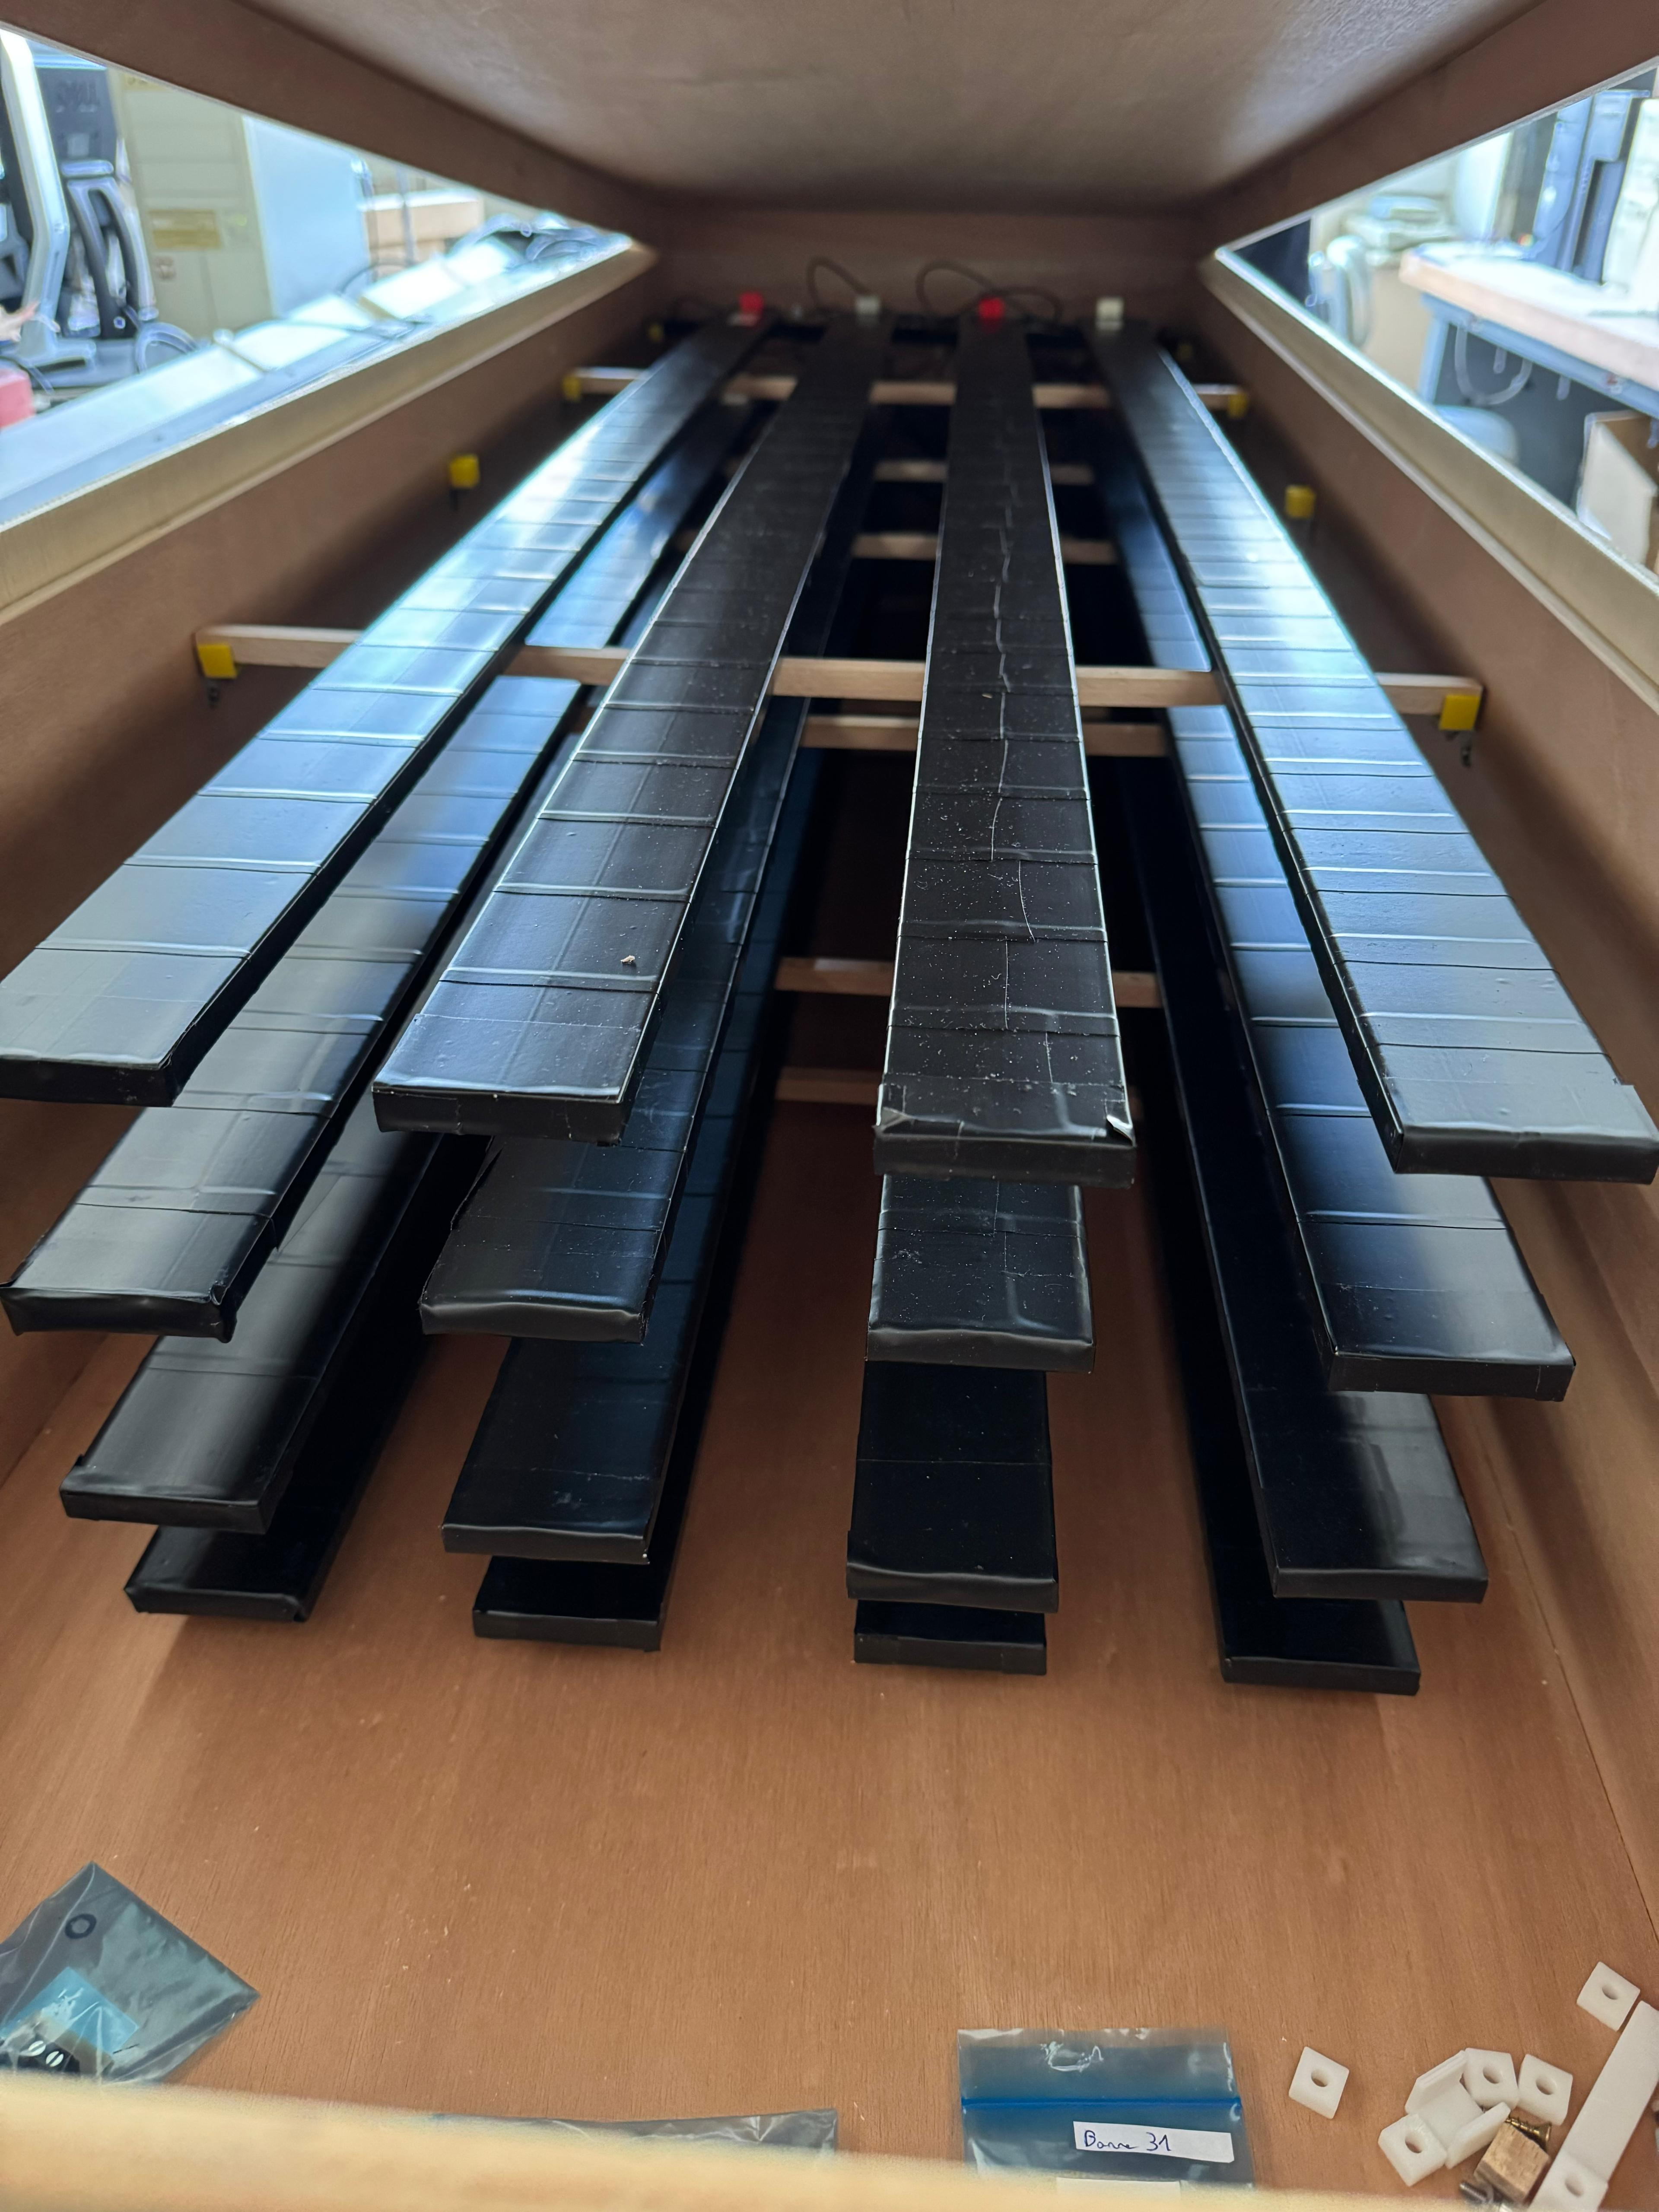
\includegraphics[width=0.3\textwidth]{Images/matrice_scint.jpg}
  \caption{Montage expérimental de la matrice de scintillateurs. On voit que les scintillateurs sont placés en quadrillage, ce qui permet de détecter les muons qui passent dans la direction des scintillateurs.}
  \label{fig:scintillateur}
\end{figure}

\begin{center}
\begin{tcolorbox}[colback=blue!5!white, colframe=blue!60!black, title=Principe de la matrice de scintillateurs]
Au lieu de déplacer les scintillateurs pour sélectionner différents angles, on utilise une matrice fixe de scintillateurs disposés en grille (\ref{fig:matrice_scintillateur}; \ref{fig:matrice_scintillateur_2}). Chaque muon traversant la matrice active une combinaison unique de scintillateurs, ce qui permet de reconstituer sa trajectoire et donc son angle d’incidence. Cette méthode permet de mesurer simultanément le flux de muons pour plusieurs directions discrètes, tout en améliorant la pureté angulaire et la statistique des mesures.
\end{tcolorbox}
\end{center}

Il faut alors prendre soin à re-optimiser les scintillateurs pour qu'ils soient tous dans la même zone de fonctionnement.

\begin{figure}[!h]
  \begin{minipage}
  {0.45\textwidth}
    \centering
    

\tikzset{every picture/.style={line width=0.75pt}} %set default line width to 0.75pt        

\begin{tikzpicture}[x=0.75pt,y=0.75pt,yscale=-1,xscale=1]
%uncomment if require: \path (0,300); %set diagram left start at 0, and has height of 300

%Shape: Rectangle [id:dp8929945080924364] 
\draw  [color={rgb, 255:red, 74; green, 74; blue, 74 }  ,draw opacity=1 ][fill={rgb, 255:red, 155; green, 155; blue, 155 }  ,fill opacity=0.76 ] (119.76,50) -- (180,50) -- (180,70) -- (119.76,70) -- cycle ;
%Shape: Rectangle [id:dp03700293554706591] 
\draw  [color={rgb, 255:red, 74; green, 74; blue, 74 }  ,draw opacity=1 ][fill={rgb, 255:red, 155; green, 155; blue, 155 }  ,fill opacity=0.76 ] (199.76,50) -- (260,50) -- (260,70) -- (199.76,70) -- cycle ;
%Shape: Rectangle [id:dp8569947057379811] 
\draw  [color={rgb, 255:red, 74; green, 74; blue, 74 }  ,draw opacity=1 ][fill={rgb, 255:red, 155; green, 155; blue, 155 }  ,fill opacity=0.76 ] (279.76,50) -- (340,50) -- (340,70) -- (279.76,70) -- cycle ;
%Shape: Rectangle [id:dp047508087293761214] 
\draw  [color={rgb, 255:red, 74; green, 74; blue, 74 }  ,draw opacity=1 ][fill={rgb, 255:red, 155; green, 155; blue, 155 }  ,fill opacity=0.76 ] (359.76,50) -- (420,50) -- (420,70) -- (359.76,70) -- cycle ;
%Shape: Rectangle [id:dp804891904862634] 
\draw  [color={rgb, 255:red, 74; green, 74; blue, 74 }  ,draw opacity=1 ][fill={rgb, 255:red, 155; green, 155; blue, 155 }  ,fill opacity=0.76 ] (359.76,90) -- (420,90) -- (420,110) -- (359.76,110) -- cycle ;
%Shape: Rectangle [id:dp7891481287882621] 
\draw  [color={rgb, 255:red, 74; green, 74; blue, 74 }  ,draw opacity=1 ][fill={rgb, 255:red, 155; green, 155; blue, 155 }  ,fill opacity=0.76 ] (359.76,130) -- (420,130) -- (420,150) -- (359.76,150) -- cycle ;
%Shape: Rectangle [id:dp8421190743551017] 
\draw  [color={rgb, 255:red, 74; green, 74; blue, 74 }  ,draw opacity=1 ][fill={rgb, 255:red, 155; green, 155; blue, 155 }  ,fill opacity=0.76 ] (280,130) -- (340.24,130) -- (340.24,150) -- (280,150) -- cycle ;
%Shape: Rectangle [id:dp3878529505907744] 
\draw  [color={rgb, 255:red, 74; green, 74; blue, 74 }  ,draw opacity=1 ][fill={rgb, 255:red, 155; green, 155; blue, 155 }  ,fill opacity=0.76 ] (280,90) -- (340.24,90) -- (340.24,110) -- (280,110) -- cycle ;
%Shape: Rectangle [id:dp2857860085693358] 
\draw  [color={rgb, 255:red, 74; green, 74; blue, 74 }  ,draw opacity=1 ][fill={rgb, 255:red, 155; green, 155; blue, 155 }  ,fill opacity=0.76 ] (200,90) -- (260.24,90) -- (260.24,110) -- (200,110) -- cycle ;
%Shape: Rectangle [id:dp30353445562744275] 
\draw  [color={rgb, 255:red, 74; green, 74; blue, 74 }  ,draw opacity=1 ][fill={rgb, 255:red, 155; green, 155; blue, 155 }  ,fill opacity=0.76 ] (200,130) -- (260.24,130) -- (260.24,150) -- (200,150) -- cycle ;
%Shape: Rectangle [id:dp6728764956214088] 
\draw  [color={rgb, 255:red, 74; green, 74; blue, 74 }  ,draw opacity=1 ][fill={rgb, 255:red, 155; green, 155; blue, 155 }  ,fill opacity=0.76 ] (120,90) -- (180.24,90) -- (180.24,110) -- (120,110) -- cycle ;
%Shape: Rectangle [id:dp08539913692996881] 
\draw  [color={rgb, 255:red, 74; green, 74; blue, 74 }  ,draw opacity=1 ][fill={rgb, 255:red, 155; green, 155; blue, 155 }  ,fill opacity=0.76 ] (120,130) -- (180.24,130) -- (180.24,150) -- (120,150) -- cycle ;

% Text Node
\draw (149.88,60) node   [align=left] {34};
% Text Node
\draw (229.88,60) node   [align=left] {33};
% Text Node
\draw (309.88,60) node   [align=left] {32};
% Text Node
\draw (150.12,100) node   [align=left] {24};
% Text Node
\draw (230.12,100) node   [align=left] {23};
% Text Node
\draw (310.12,100) node   [align=left] {22};
% Text Node
\draw (389.88,100) node   [align=left] {21};
% Text Node
\draw (389.88,60) node   [align=left] {31};
% Text Node
\draw (389.88,140) node   [align=left] {11};
% Text Node
\draw (310.12,140) node   [align=left] {12};
% Text Node
\draw (230.12,140) node   [align=left] {13};
% Text Node
\draw (150.12,140) node   [align=left] {14};


\end{tikzpicture}

    \caption{Configuration de la matrice des scintillateurs. Chaque scintillateur est indéxé a la maniere des coeficients d'une matrice.}
    \label{fig:matrice_scintillateur}
  \end{minipage}
  \hfill
  \begin{minipage}{0.45\textwidth}
    \centering
    

\tikzset{every picture/.style={line width=0.75pt}} %set default line width to 0.75pt        

\begin{tikzpicture}[x=0.75pt,y=0.75pt,yscale=-1,xscale=1]
%uncomment if require: \path (0,300); %set diagram left start at 0, and has height of 300

%Shape: Rectangle [id:dp9677752234257792] 
\draw  [color={rgb, 255:red, 74; green, 74; blue, 74 }  ,draw opacity=1 ][fill={rgb, 255:red, 155; green, 155; blue, 155 }  ,fill opacity=0.76 ] (119.76,50) -- (180,50) -- (180,70) -- (119.76,70) -- cycle ;
%Shape: Rectangle [id:dp7783045174475527] 
\draw  [color={rgb, 255:red, 74; green, 74; blue, 74 }  ,draw opacity=1 ][fill={rgb, 255:red, 155; green, 155; blue, 155 }  ,fill opacity=0.76 ] (199.76,50) -- (260,50) -- (260,70) -- (199.76,70) -- cycle ;
%Shape: Rectangle [id:dp2916565511058188] 
\draw  [color={rgb, 255:red, 74; green, 74; blue, 74 }  ,draw opacity=1 ][fill={rgb, 255:red, 155; green, 155; blue, 155 }  ,fill opacity=0.76 ] (279.76,50) -- (340,50) -- (340,70) -- (279.76,70) -- cycle ;
%Shape: Rectangle [id:dp6887263347251699] 
\draw  [color={rgb, 255:red, 74; green, 74; blue, 74 }  ,draw opacity=1 ][fill={rgb, 255:red, 155; green, 155; blue, 155 }  ,fill opacity=0.76 ] (359.76,50) -- (420,50) -- (420,70) -- (359.76,70) -- cycle ;
%Shape: Rectangle [id:dp7312242099062684] 
\draw  [color={rgb, 255:red, 74; green, 74; blue, 74 }  ,draw opacity=1 ][fill={rgb, 255:red, 155; green, 155; blue, 155 }  ,fill opacity=0.76 ] (359.76,90) -- (420,90) -- (420,110) -- (359.76,110) -- cycle ;
%Shape: Rectangle [id:dp3236731708710169] 
\draw  [color={rgb, 255:red, 74; green, 74; blue, 74 }  ,draw opacity=1 ][fill={rgb, 255:red, 155; green, 155; blue, 155 }  ,fill opacity=0.76 ] (359.76,130) -- (420,130) -- (420,150) -- (359.76,150) -- cycle ;
%Shape: Rectangle [id:dp46880323529823853] 
\draw  [color={rgb, 255:red, 74; green, 74; blue, 74 }  ,draw opacity=1 ][fill={rgb, 255:red, 155; green, 155; blue, 155 }  ,fill opacity=0.76 ] (280,130) -- (340.24,130) -- (340.24,150) -- (280,150) -- cycle ;
%Shape: Rectangle [id:dp7337467153729857] 
\draw  [color={rgb, 255:red, 74; green, 74; blue, 74 }  ,draw opacity=1 ][fill={rgb, 255:red, 155; green, 155; blue, 155 }  ,fill opacity=0.76 ] (280,90) -- (340.24,90) -- (340.24,110) -- (280,110) -- cycle ;
%Shape: Rectangle [id:dp6938832339212349] 
\draw  [color={rgb, 255:red, 74; green, 74; blue, 74 }  ,draw opacity=1 ][fill={rgb, 255:red, 155; green, 155; blue, 155 }  ,fill opacity=0.76 ] (200,90) -- (260.24,90) -- (260.24,110) -- (200,110) -- cycle ;
%Shape: Rectangle [id:dp2812215450878759] 
\draw  [color={rgb, 255:red, 74; green, 74; blue, 74 }  ,draw opacity=1 ][fill={rgb, 255:red, 155; green, 155; blue, 155 }  ,fill opacity=0.76 ] (200,130) -- (260.24,130) -- (260.24,150) -- (200,150) -- cycle ;
%Shape: Rectangle [id:dp7929517313076475] 
\draw  [color={rgb, 255:red, 74; green, 74; blue, 74 }  ,draw opacity=1 ][fill={rgb, 255:red, 155; green, 155; blue, 155 }  ,fill opacity=0.76 ] (120,90) -- (180.24,90) -- (180.24,110) -- (120,110) -- cycle ;
%Shape: Rectangle [id:dp17968757590374962] 
\draw  [color={rgb, 255:red, 74; green, 74; blue, 74 }  ,draw opacity=1 ][fill={rgb, 255:red, 155; green, 155; blue, 155 }  ,fill opacity=0.76 ] (120,130) -- (180.24,130) -- (180.24,150) -- (120,150) -- cycle ;
%Straight Lines [id:da8414412126257806] 
\draw [color={rgb, 255:red, 208; green, 2; blue, 27 }  ,draw opacity=1 ][line width=2.25]    (120,50) -- (340,150) ;
\draw [shift={(230,100)}, rotate = 204.44] [color={rgb, 255:red, 208; green, 2; blue, 27 }  ,draw opacity=1 ][line width=2.25]    (28.22,-7.84) .. controls (21.85,-3.68) and (16.03,-1.07) .. (10.74,0) .. controls (16.03,1.07) and (21.85,3.68) .. (28.22,7.84)(17.49,-7.84) .. controls (11.12,-3.68) and (5.29,-1.07) .. (0,0) .. controls (5.29,1.07) and (11.12,3.68) .. (17.49,7.84)   ;
%Straight Lines [id:da3854874229182752] 
\draw [color={rgb, 255:red, 144; green, 19; blue, 254 }  ,draw opacity=1 ][line width=2.25]    (199.76,50) -- (420,110) ;
\draw [shift={(309.88,80)}, rotate = 195.24] [color={rgb, 255:red, 144; green, 19; blue, 254 }  ,draw opacity=1 ][line width=2.25]    (28.22,-7.84) .. controls (21.85,-3.68) and (16.03,-1.07) .. (10.74,0) .. controls (16.03,1.07) and (21.85,3.68) .. (28.22,7.84)(17.49,-7.84) .. controls (11.12,-3.68) and (5.29,-1.07) .. (0,0) .. controls (5.29,1.07) and (11.12,3.68) .. (17.49,7.84)   ;
%Straight Lines [id:da8454035078662195] 
\draw [color={rgb, 255:red, 65; green, 117; blue, 5 }  ,draw opacity=1 ][line width=2.25]    (390,50) -- (390,150) ;
\draw [shift={(390,100)}, rotate = 270] [color={rgb, 255:red, 65; green, 117; blue, 5 }  ,draw opacity=1 ][line width=2.25]    (28.22,-7.84) .. controls (21.85,-3.68) and (16.03,-1.07) .. (10.74,0) .. controls (16.03,1.07) and (21.85,3.68) .. (28.22,7.84)(17.49,-7.84) .. controls (11.12,-3.68) and (5.29,-1.07) .. (0,0) .. controls (5.29,1.07) and (11.12,3.68) .. (17.49,7.84)   ;

% Text Node
\draw (149.88,60) node   [align=left] {34};
% Text Node
\draw (229.88,60) node   [align=left] {33};
% Text Node
\draw (309.88,60) node   [align=left] {32};
% Text Node
\draw (150.12,100) node   [align=left] {24};
% Text Node
\draw (230.12,100) node   [align=left] {23};
% Text Node
\draw (310.12,100) node   [align=left] {22};
% Text Node
\draw (389.88,100) node   [align=left] {21};
% Text Node
\draw (389.88,60) node   [align=left] {31};
% Text Node
\draw (389.88,140) node   [align=left] {11};
% Text Node
\draw (310.12,140) node   [align=left] {12};
% Text Node
\draw (230.12,140) node   [align=left] {13};
% Text Node
\draw (150.12,140) node   [align=left] {14};


\end{tikzpicture}

    \caption{Exemple de trajectoire d'un muon dans la matrice de scintillateurs.\\On voit que le muon traverse plusieurs scintillateurs, ce qui permet de le détecter uniquement certains angles dicrets. Ici en rouge $\theta = 0.989 rad$, en violet $\theta = 1.36 rad$ et en bleu $\theta = 0 rad$.}
    \label{fig:matrice_scintillateur_2}
  \end{minipage}
\end{figure}

Il s'agit de choisir le bon treshold. Nous avons commencé par tracer grossierement les caractéristiques de deux scintillateurs aleatoirement choisis. Ces résultats sont representés figure \ref{fig:caracteristique_scintillateur_2}.
 On appercoit qu'ils ont sensiblement les mêmes caractéristiques. On suppose donc que, étant de  même facture, tous se comportent sensiblement pareil. On pose donc un treshold à \textbf{TRHS = 22mV}.

\begin{figure}[!h]
  \begin{minipage}
  {0.45\textwidth}
    \centering
    \includegraphics[width=0.9\textwidth]{Images/palier_dezoomé.png}
    \caption{Caractéristique du scintillateur des scintillateurs 21 et 34. On appercoit mieux les courbes attendues avec la presence d'un palier au alentours des memes valeures.}
    \label{fig:caracteristique_scintillateur_1}
  \end{minipage}
  \hfill
  \begin{minipage}{0.45\textwidth}
    \centering
    \includegraphics[width=0.9\textwidth]{Images/palier_zommé.png}
    \caption{Caractéristique du scintillateur des scintillateurs zommé sur la zone du palier. On observbe la chute de counts pour un seuil trop haut apres le palier. Le détetecteur 34 a l'aire plus efficace que le 21. On suppoose alors que tout les scintillatyeurs on sensiblement les mêmes caractéristiques et on choisit pour le reste de l'étude THRS = 22mv}
    \label{fig:caracteristique_scintillateur_2}
  \end{minipage}
\end{figure}

On peut alors lancer une longue acquisition de données. 
On a pris soin de bien choisir la zone de fonctionnement des scintillateurs pour qu'ils soient tous dans la meme zone de fonctionnement. 
On analyse alors les données et on trace les occurences des angles en fonction de l'angle pour essayer de verifier la loi $\cos^2\theta$.
Il faut faire attention a bien normaliser les résultats en fonction du nombre de combinaisons possibles correspondantes pour chaque angle.
Les résultats obtenus sont représentés figure \ref{fig:cos2s_2}.

\begin{figure}[H]
  \centering
  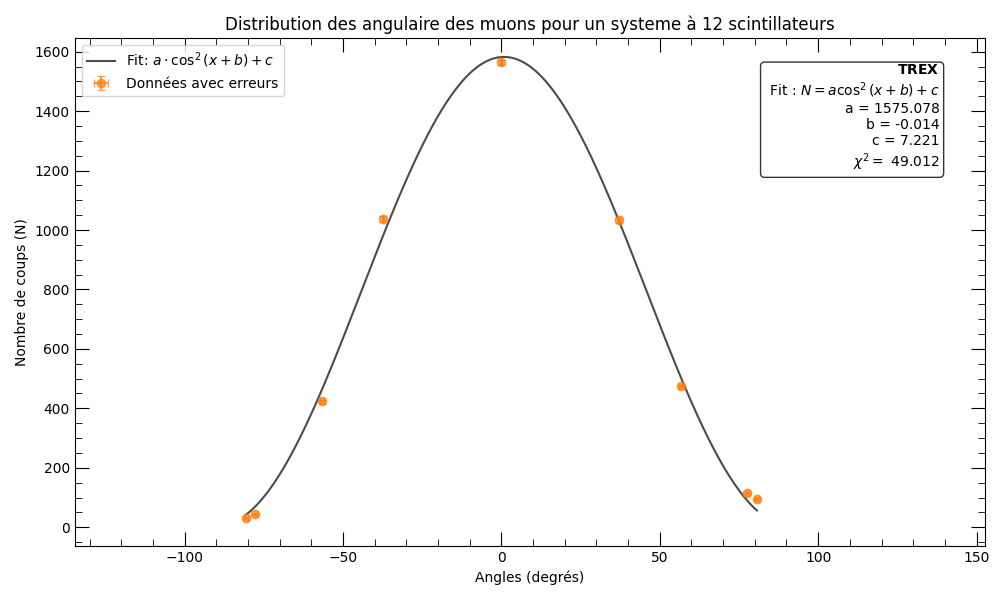
\includegraphics[width=0.7\textwidth]{Images/distribution_angulaire.png}
  \caption{Nombre de muons corrigé par le nombre de combinaisons possibles mesuré en fonction de l'angle d'incidence $\theta$. On observe une décroissance du flux avec l'angle, confirmant la loi $\cos^2\theta$. On note l'écartement au modèle aux grands angles.
  On note aussi la différence de qualité des mesures entre 3 scintillateurs et la matrice de scintillateurs.}
  \label{fig:cos2s_2}
\end{figure}


\section{Mesure de l’énergie d’un muon}
\begin{center}
\begin{tcolorbox}[colback=blue!5!white, colframe=blue!60!black, title=Principe de la mesure de l'énergie des muons cosmiques]
L’expérience consiste à interposer des plaques de plomb de différentes épaisseurs entre le flux de muons cosmiques et un détecteur à scintillateurs. Seuls les muons possédant une énergie suffisante pour traverser toute l’épaisseur de plomb sont détectés. Ainsi, en augmentant progressivement l’épaisseur de plomb et en mesurant le nombre de muons détectés, on observe une diminution du flux mesuré. Cette atténuation permet d’obtenir des informations sur la distribution en énergie des muons cosmiques : plus l’épaisseur est grande, plus seuls les muons les plus énergétiques sont comptés.
\end{tcolorbox}
\end{center}


On mesure donc le nombre de coups par minute $N(x)$ en fonction de l’épaisseur de plomb $x$.
 À chaque valeur de $x$, on associe une énergie minimale $E_{\min}(x)$ nécessaire pour traverser cette épaisseur, estimée par $E_{\min}(x) \approx \frac{dE}{dx} \cdot x \approx 19.3 \cdot x$ (en MeV), en supposant une perte d’énergie moyenne constante dans le plomb.

L’analyse des données repose sur l’ajustement de la courbe $N(x)$ selon une loi de puissance dérivée du spectre attendu des muons cosmiques : $N(E_{\min}) \propto E_{\min}^{1 - \gamma}$, avec $\gamma \approx 2.7$.Cela est représenté figure \ref{fig:energie_fit}.On voit que la loi n'est pas pas retrouvé ce qui est du aux imprécisions des mesures, mais le même ordre de grandeur est retrouvé.

Cependant, on observe parfois une \textit{hausse du nombre de coups pour de faibles épaisseurs de plomb}. Ce phénomène s’explique par des \textit{interactions secondaires} : les muons (ou autres particules) peuvent interagir dans le plomb et produire des électrons, photons (rayonnement de freinage), ou autres particules secondaires, qui peuvent elles-mêmes être détectées par les scintillateurs. Ces événements parasites peuvent fausser les mesures et doivent être pris en compte dans l’interprétation des résultats.

\begin{figure}[!h]
  \begin{minipage}
  {0.49\textwidth}
  \centering
  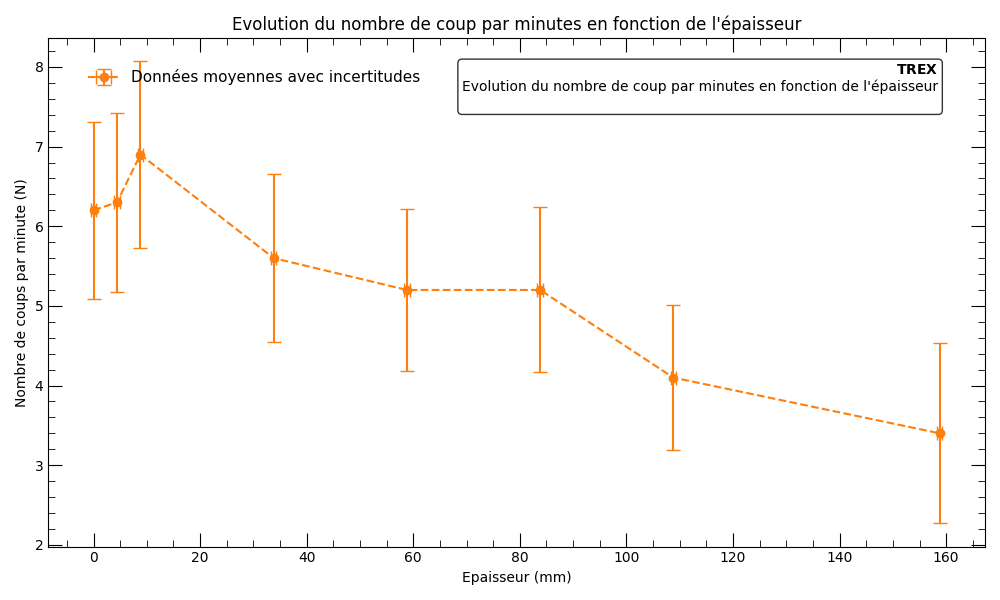
\includegraphics[width=0.9\textwidth]{Images/energie.png}
  \caption{Le nombre de coups diminue globalement avec l’épaisseur, traduisant l’atténuation des muons. Une légère hausse initiale peut être observée, due à la production de particules secondaires dans le plomb, susceptibles d’être détectées par les scintillateurs }

  \label{fig:energie_1}
  \end{minipage}
  \hfill
  \begin{minipage}{0.45\textwidth}
  \centering
  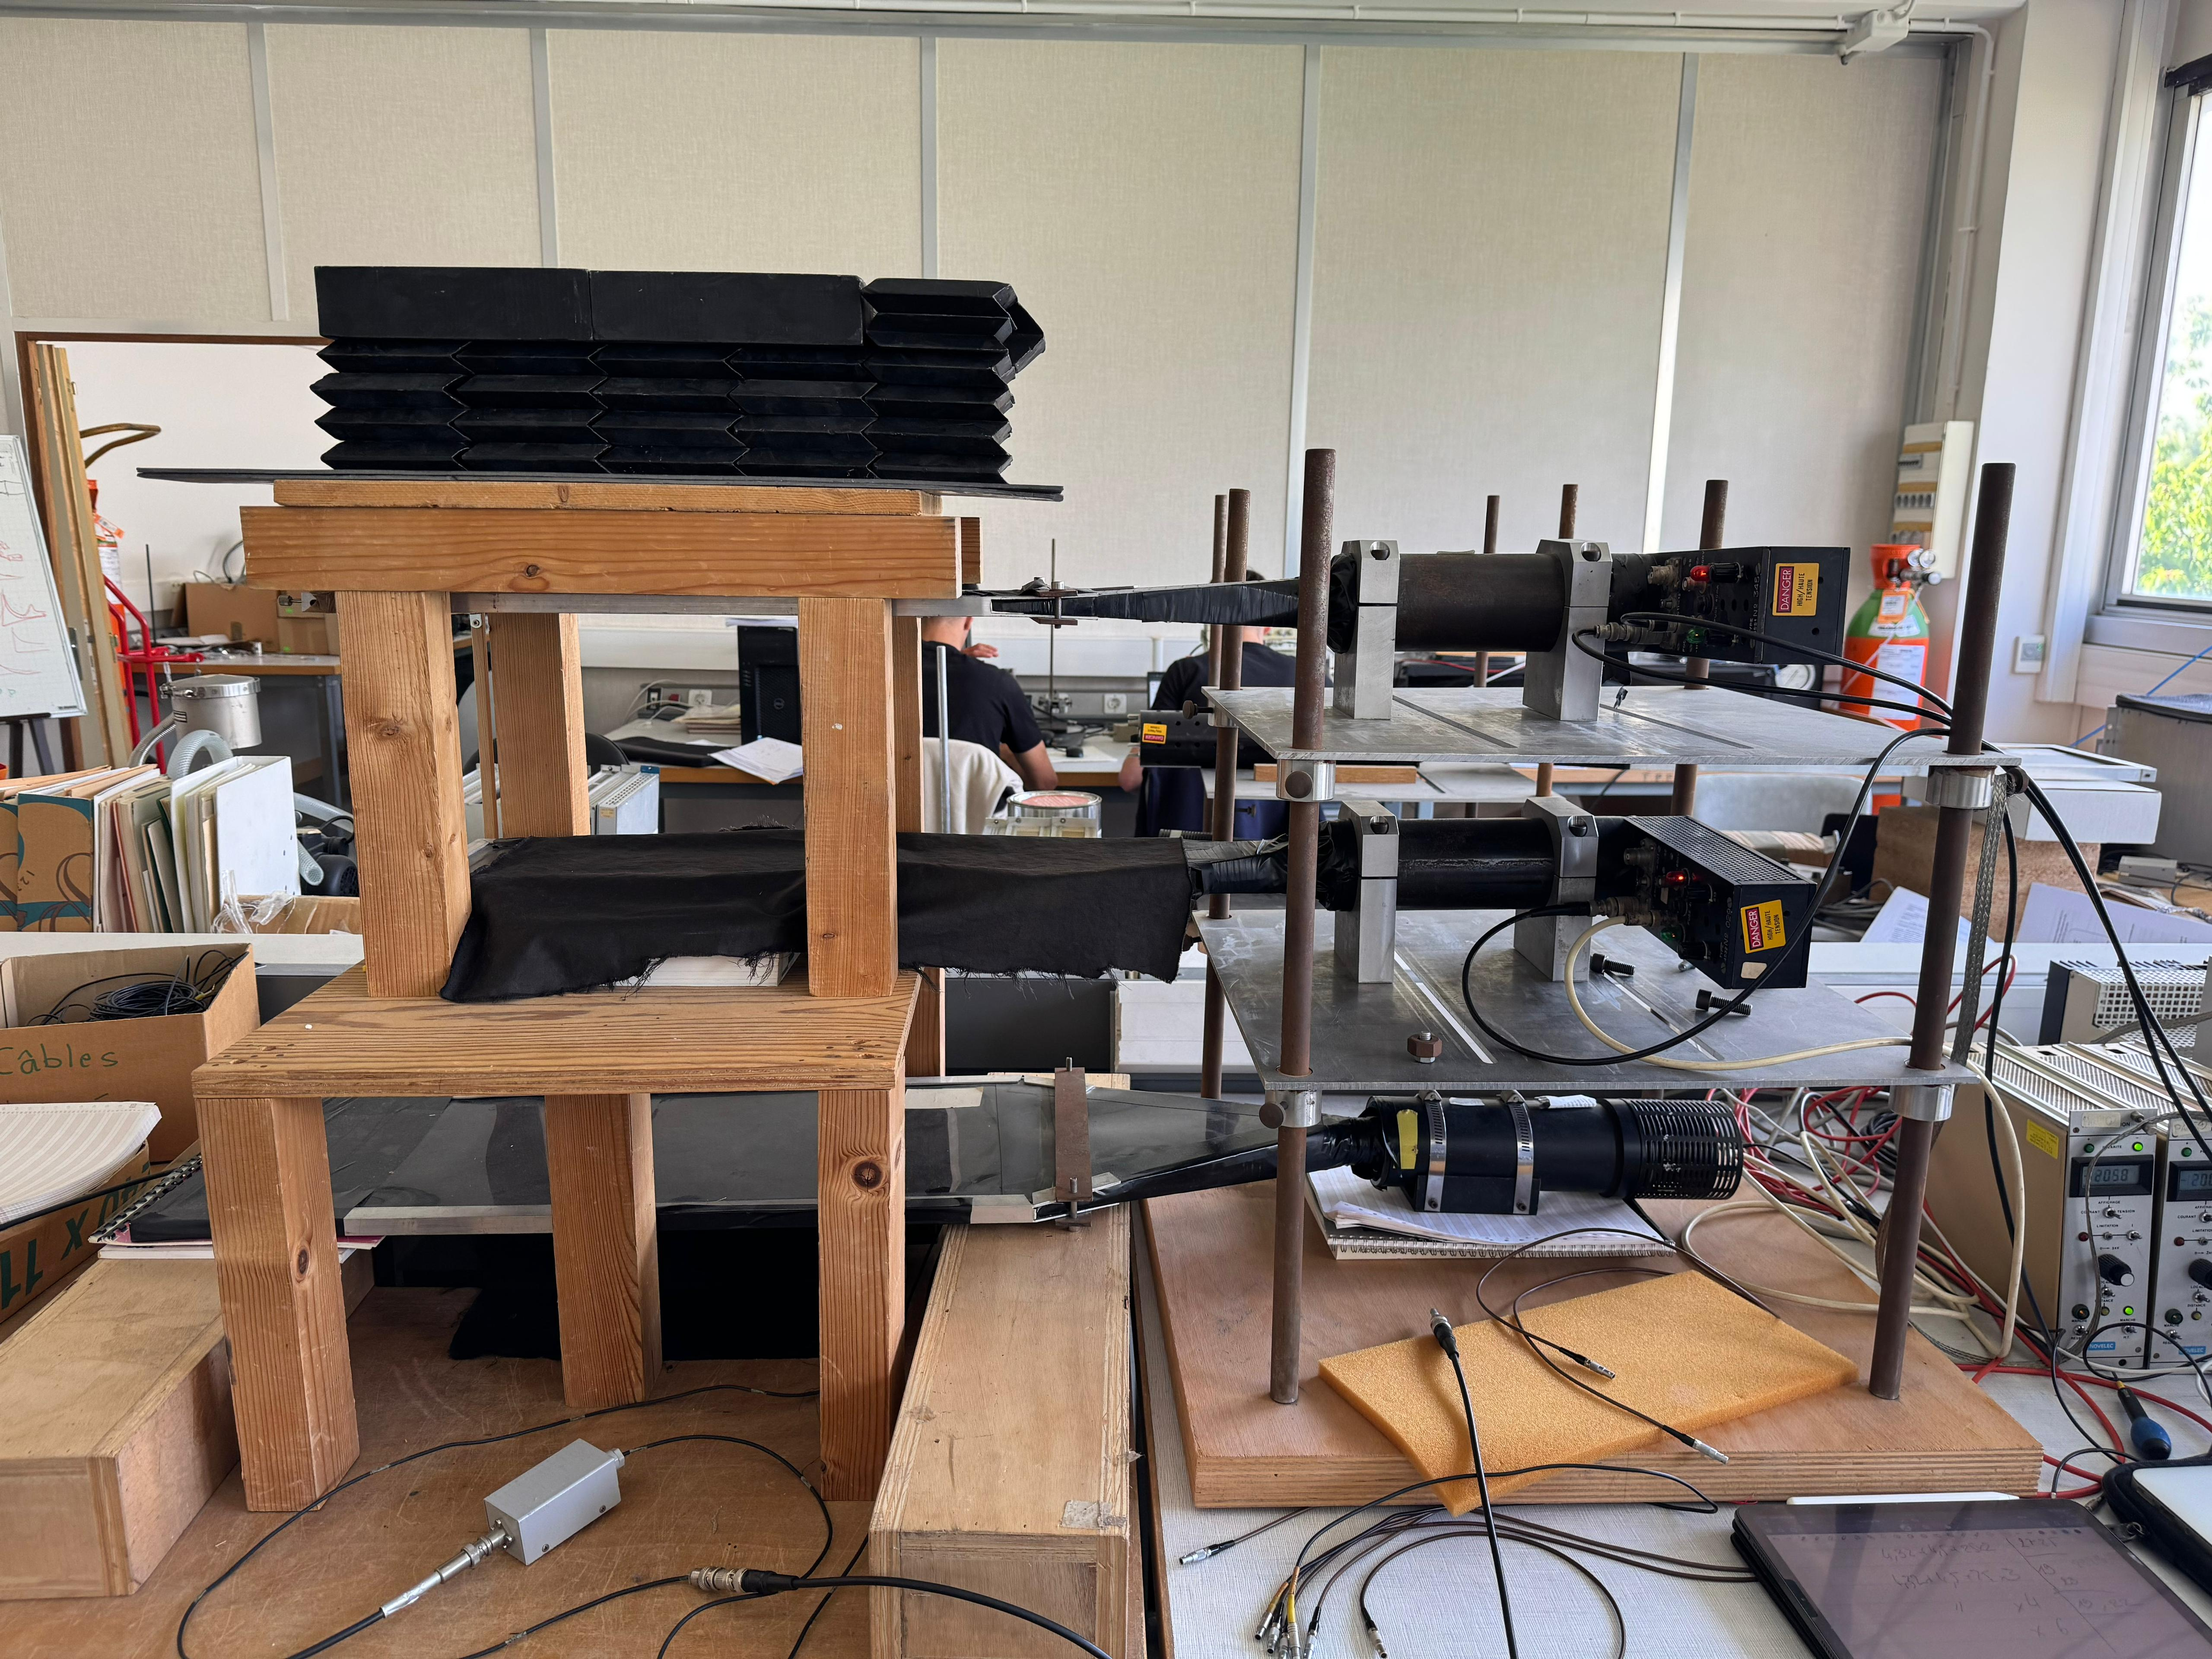
\includegraphics[width=0.7\textwidth]{Images/plomb.jpg}
  \caption{Montage expérimental pour la mesure de l’énergie des muons. On place des plaques de plomb de différentes épaisseurs au dessus des scintillateurs.}
  \label{fig:energie_2}
  \end{minipage}
  \end{figure}
Les muons cosmiques perdent leur énergie dans la matière principalement par \textit{ionisation} et \textit{excitation des atomes}, mécanismes dominants à des énergies intermédiaires (de quelques centaines de MeV à quelques GeV). À plus haute énergie, des processus radiatifs comme le \textit{bremsstrahlung}, la \textit{production de paires} ou des \textit{interactions hadroniques} avec les noyaux peuvent également contribuer. Ces processus peuvent générer des \textit{particules secondaires} (électrons, photons, pions, neutrons...) susceptibles d’être détectées par les scintillateurs, en particulier dans les premières couches de plomb. Ce mécanisme explique l’excès de comptage observé pour de faibles épaisseurs.

\begin{center}
\begin{tcolorbox}[colback=red!5!white, colframe=red!80!black, title=Problèmes et limitations de la mesure de l'énergie des muons cosmiques]
La mesure de l’énergie des muons par atténuation dans le plomb présente plusieurs difficultés expérimentales :
\begin{itemize}
    \item \textbf{Production de particules secondaires~:} Les muons (ou autres particules) peuvent interagir dans le plomb et produire des électrons ou photons secondaires, qui sont aussi détectés par les scintillateurs. Cela fausse le comptage, surtout pour les faibles épaisseurs de plomb.
    \item \textbf{Statistique limitée~:} Le flux de muons suffisamment énergétiques pour traverser de grandes épaisseurs de plomb est faible, ce qui impose des temps d’acquisition longs et augmente l’incertitude statistique.
    \item \textbf{Imprécisions sur l’épaisseur et l’alignement~:} Les tolérances sur l’épaisseur réelle du plomb et l’alignement des plaques peuvent introduire des erreurs systématiques sur l’énergie minimale estimée.
    \item \textbf{Hypothèses simplificatrices~:} L’estimation de l’énergie minimale repose sur une perte d’énergie moyenne constante ($dE/dx$), alors qu’en réalité il existe des fluctuations importantes (straggling) et des contributions variables selon l’énergie.
    \item \textbf{Bruit de fond et coïncidences accidentelles~:} Des événements parasites (radioactivité, bruit électronique) peuvent être comptés à tort comme des muons traversant le plomb, surtout pour les faibles taux de comptage.
\end{itemize}
Ces limitations expliquent les écarts observés entre la loi théorique et les résultats expérimentaux, et imposent une interprétation prudente des mesures.
\end{tcolorbox}
\end{center}

\begin{figure}[!h]
  \centering
  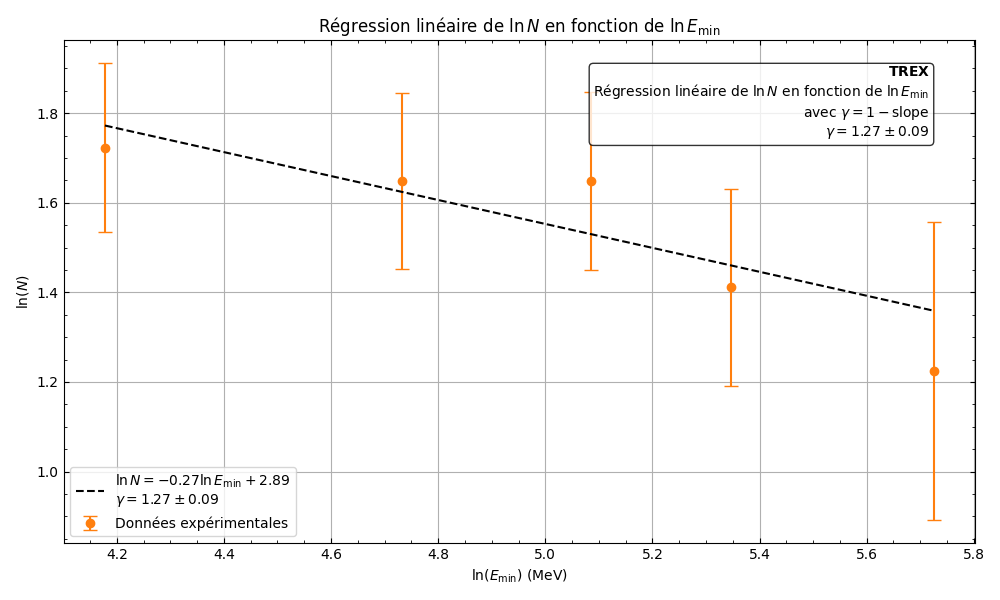
\includegraphics[width=0.7\textwidth]{Images/plot_gamma.png}
  \caption{On trace $\ln N$ en fonction de $\ln E_{\min}$. L’ajustement par une droite permet d’estimer l’exposant $\gamma$ du spectre des muons.
  On voit que la loi ne puissance n'est pas du tout vérifié (même si l'ordre de grandeur est le même). Cela est surrement du au petite epaisseurs de plombs qui ont pu etre mises en place et aussi à l'imprecision globale des mesures.}
  \label{fig:energie_fit}
\end{figure}

\section{Mesure du temps de vie de muon}

\begin{figure}
  \centering
  

\tikzset{every picture/.style={line width=0.75pt}} %set default line width to 0.75pt        

\begin{tikzpicture}[x=0.75pt,y=0.75pt,yscale=-1,xscale=1]
%uncomment if require: \path (0,300); %set diagram left start at 0, and has height of 300

%Straight Lines [id:da16127255456541323] 
\draw [color={rgb, 255:red, 0; green, 0; blue, 0 }  ,draw opacity=1 ][fill={rgb, 255:red, 245; green, 166; blue, 35 }  ,fill opacity=1 ][line width=1.5]    (176,49) -- (265,49) ;
\draw [shift={(263,49)}, rotate = 0] [fill={rgb, 255:red, 0; green, 0; blue, 0 }  ,fill opacity=1 ][line width=0.08]  [draw opacity=0] (13.4,-6.43) -- (0,0) -- (13.4,6.44) -- (8.9,0) -- cycle    ;
\draw [shift={(178,49)}, rotate = 180] [fill={rgb, 255:red, 0; green, 0; blue, 0 }  ,fill opacity=1 ][line width=0.08]  [draw opacity=0] (13.4,-6.43) -- (0,0) -- (13.4,6.44) -- (8.9,0) -- cycle    ;
%Straight Lines [id:da7982807003028938] 
\draw [color={rgb, 255:red, 0; green, 0; blue, 0 }  ,draw opacity=1 ][fill={rgb, 255:red, 245; green, 166; blue, 35 }  ,fill opacity=1 ][line width=1.5]    (176,70) -- (265,70) ;
\draw [shift={(263,70)}, rotate = 0] [fill={rgb, 255:red, 0; green, 0; blue, 0 }  ,fill opacity=1 ][line width=0.08]  [draw opacity=0] (13.4,-6.43) -- (0,0) -- (13.4,6.44) -- (8.9,0) -- cycle    ;
\draw [shift={(178,70)}, rotate = 180] [fill={rgb, 255:red, 0; green, 0; blue, 0 }  ,fill opacity=1 ][line width=0.08]  [draw opacity=0] (13.4,-6.43) -- (0,0) -- (13.4,6.44) -- (8.9,0) -- cycle    ;
%Straight Lines [id:da08370009723597649] 
\draw [color={rgb, 255:red, 0; green, 0; blue, 0 }  ,draw opacity=1 ][fill={rgb, 255:red, 245; green, 166; blue, 35 }  ,fill opacity=1 ][line width=1.5]    (176,91) -- (265,91) ;
\draw [shift={(263,91)}, rotate = 0] [fill={rgb, 255:red, 0; green, 0; blue, 0 }  ,fill opacity=1 ][line width=0.08]  [draw opacity=0] (13.4,-6.43) -- (0,0) -- (13.4,6.44) -- (8.9,0) -- cycle    ;
\draw [shift={(178,91)}, rotate = 180] [fill={rgb, 255:red, 0; green, 0; blue, 0 }  ,fill opacity=1 ][line width=0.08]  [draw opacity=0] (13.4,-6.43) -- (0,0) -- (13.4,6.44) -- (8.9,0) -- cycle    ;
%Shape: Bevel [id:dp6673775601267844] 
\draw   (175,105) -- (266,105) -- (266,133) -- (175,133) -- cycle ; \draw   (177.92,107.92) -- (263.08,107.92) -- (263.08,130.08) -- (177.92,130.08) -- cycle ; \draw   (175,105) -- (177.92,107.92) ; \draw   (266,105) -- (263.08,107.92) ; \draw   (266,133) -- (263.08,130.08) ; \draw   (175,133) -- (177.92,130.08) ;
%Straight Lines [id:da29762688824856964] 
\draw [color={rgb, 255:red, 208; green, 2; blue, 27 }  ,draw opacity=1 ]   (222,28) .. controls (223.67,29.67) and (223.67,31.33) .. (222,33) .. controls (220.33,34.67) and (220.33,36.33) .. (222,38) .. controls (223.67,39.67) and (223.67,41.33) .. (222,43) .. controls (220.33,44.67) and (220.33,46.33) .. (222,48) .. controls (223.67,49.67) and (223.67,51.33) .. (222,53) .. controls (220.33,54.67) and (220.33,56.33) .. (222,58) .. controls (223.67,59.67) and (223.67,61.33) .. (222,63) .. controls (220.33,64.67) and (220.33,66.33) .. (222,68) .. controls (223.67,69.67) and (223.67,71.33) .. (222,73) .. controls (220.33,74.67) and (220.33,76.33) .. (222,78) .. controls (223.67,79.67) and (223.67,81.33) .. (222,83) .. controls (220.33,84.67) and (220.33,86.33) .. (222,88) .. controls (223.67,89.67) and (223.67,91.33) .. (222,93) .. controls (220.33,94.67) and (220.33,96.33) .. (222,98) .. controls (223.67,99.67) and (223.67,101.33) .. (222,103) .. controls (220.33,104.67) and (220.33,106.33) .. (222,108) -- (222,111)(219,28) .. controls (220.67,29.67) and (220.67,31.33) .. (219,33) .. controls (217.33,34.67) and (217.33,36.33) .. (219,38) .. controls (220.67,39.67) and (220.67,41.33) .. (219,43) .. controls (217.33,44.67) and (217.33,46.33) .. (219,48) .. controls (220.67,49.67) and (220.67,51.33) .. (219,53) .. controls (217.33,54.67) and (217.33,56.33) .. (219,58) .. controls (220.67,59.67) and (220.67,61.33) .. (219,63) .. controls (217.33,64.67) and (217.33,66.33) .. (219,68) .. controls (220.67,69.67) and (220.67,71.33) .. (219,73) .. controls (217.33,74.67) and (217.33,76.33) .. (219,78) .. controls (220.67,79.67) and (220.67,81.33) .. (219,83) .. controls (217.33,84.67) and (217.33,86.33) .. (219,88) .. controls (220.67,89.67) and (220.67,91.33) .. (219,93) .. controls (217.33,94.67) and (217.33,96.33) .. (219,98) .. controls (220.67,99.67) and (220.67,101.33) .. (219,103) .. controls (217.33,104.67) and (217.33,106.33) .. (219,108) -- (219,111) ;
\draw [shift={(220.5,119)}, rotate = 270] [color={rgb, 255:red, 208; green, 2; blue, 27 }  ,draw opacity=1 ][line width=0.75]    (10.93,-3.29) .. controls (6.95,-1.4) and (3.31,-0.3) .. (0,0) .. controls (3.31,0.3) and (6.95,1.4) .. (10.93,3.29)   ;
%Curve Lines [id:da09987540810032502] 
\draw    (266,49) .. controls (266.44,-2.91) and (303,100) .. (343,70) ;
%Curve Lines [id:da8848703749954069] 
\draw    (266,91) .. controls (273.16,69.09) and (303,100) .. (343,70) ;
%Curve Lines [id:da6551396221292157] 
\draw    (266,70) .. controls (276.62,40) and (300.25,98.36) .. (343,70) ;
%Curve Lines [id:da5197903529881432] 
\draw    (266,119) .. controls (295.2,97.2) and (313.77,126.34) .. (343,91) ;
%Shape: Frame [id:dp11732449683870594] 
\draw   (343,49) -- (448,49) -- (448,112) -- (343,112) -- cycle(444.38,52.62) -- (346.62,52.62) -- (346.62,108.38) -- (444.38,108.38) -- cycle ;
%Curve Lines [id:da21062541779004906] 
\draw [color={rgb, 255:red, 208; green, 2; blue, 27 }  ,draw opacity=1 ]   (353,91) .. controls (366.77,89.34) and (358.63,112.63) .. (364,105) ;
%Curve Lines [id:da9677935870249211] 
\draw [color={rgb, 255:red, 144; green, 19; blue, 254 }  ,draw opacity=1 ]   (378,70) .. controls (364.06,69.49) and (362.91,78.34) .. (359,84) ;
%Curve Lines [id:da3394041776120852] 
\draw [color={rgb, 255:red, 208; green, 2; blue, 27 }  ,draw opacity=1 ]   (383,91) .. controls (369.06,90.49) and (367.91,99.34) .. (364,105) ;
%Curve Lines [id:da26392268148649634] 
\draw [color={rgb, 255:red, 208; green, 2; blue, 27 }  ,draw opacity=1 ]   (436,91) .. controls (422.06,90.49) and (420.91,99.34) .. (417,105) ;
%Curve Lines [id:da3170576792274794] 
\draw [color={rgb, 255:red, 144; green, 19; blue, 254 }  ,draw opacity=1 ]   (348,70) .. controls (361.77,68.34) and (353.63,91.63) .. (359,84) ;
%Curve Lines [id:da6469687920551798] 
\draw [color={rgb, 255:red, 208; green, 2; blue, 27 }  ,draw opacity=1 ]   (406,91) .. controls (419.77,89.34) and (411.63,112.63) .. (417,105) ;
%Straight Lines [id:da18630405985817278] 
\draw [color={rgb, 255:red, 144; green, 19; blue, 254 }  ,draw opacity=1 ]   (378,70) -- (444,70) ;
%Straight Lines [id:da8977881004274828] 
\draw [color={rgb, 255:red, 208; green, 2; blue, 27 }  ,draw opacity=1 ]   (382,91) -- (406,91) ;
%Straight Lines [id:da4750464176715349] 
\draw [color={rgb, 255:red, 208; green, 2; blue, 27 }  ,draw opacity=1 ]   (436,91) -- (444,91) ;
%Straight Lines [id:da15684561527929552] 
\draw [color={rgb, 255:red, 208; green, 2; blue, 27 }  ,draw opacity=1 ]   (347,91) -- (354,91) ;
%Straight Lines [id:da7885483833241824] 
\draw [color={rgb, 255:red, 144; green, 19; blue, 254 }  ,draw opacity=1 ]   (346,70) -- (350,70) ;
%Straight Lines [id:da39695529554469833] 
\draw    (372,84) -- (413,84) ;
\draw [shift={(413,84)}, rotate = 180] [color={rgb, 255:red, 0; green, 0; blue, 0 }  ][line width=0.75]    (0,5.59) -- (0,-5.59)(10.93,-3.29) .. controls (6.95,-1.4) and (3.31,-0.3) .. (0,0) .. controls (3.31,0.3) and (6.95,1.4) .. (10.93,3.29)   ;
\draw [shift={(372,84)}, rotate = 0] [color={rgb, 255:red, 0; green, 0; blue, 0 }  ][line width=0.75]    (0,5.59) -- (0,-5.59)(10.93,-3.29) .. controls (6.95,-1.4) and (3.31,-0.3) .. (0,0) .. controls (3.31,0.3) and (6.95,1.4) .. (10.93,3.29)   ;

% Text Node
\draw (169,35) node   [align=left] {\begin{minipage}[lt]{68pt}\setlength\topsep{0pt}
\footnotesize{Scintillateurs}
\end{minipage}};
% Text Node
\draw (274,31) node   [align=left] {\begin{minipage}[lt]{68pt}\setlength\topsep{0pt}
\footnotesize{Muon}
\end{minipage}};
% Text Node
\draw (228,150) node   [align=left] {\begin{minipage}[lt]{77.52pt}\setlength\topsep{0pt}
\footnotesize{verre-au-plomb}
\end{minipage}};
% Text Node
\draw (367.5,120) node   [align=left] {{\tiny interactions muons-plomb}};
% Text Node
\draw (450,135) node   [align=left] {{\tiny désintergration du muon}};
% Text Node
\draw (357.5,35) node   [align=left] {{\tiny coincidence}};
% Text Node
\draw (485,90) node   [align=left] {{\tiny temps de vie}\\};


\end{tikzpicture}

  \caption{Principe de la mesure du temps de vie du muon.
On place un absorbeur épais (ici en verre au plomb) pour arrêter les muons, et on mesure le temps écoulé jusqu'à la désintégration. Le verre au plomb créé deux siganux: un premier lorsdque le muon interragit avec lui, un deuxieme lors de la desintegration de muon. Il faut donc discriminer ce premier signal, ce qui est fait avec l'ajout d'un délais epsilonesque par rapport au temps de vie du muon.} 
  \label{fig:muon_lifetime}
\end{figure}


\begin{center}
\begin{tcolorbox}[colback=blue!5!white, colframe=blue!60!black, title=Principe de la mesure du temps de vie du muon]
Un muon cosmique qui s’arrête dans l’absorbeur se désintègre avec une probabilité décroissant exponentiellement : $P(t)=\exp(-t/\tau_\mu)$ où $\tau_\mu\simeq2{,}2~\mu\text{s}$.  
Le \textit{start} est déclenché quand le muon traverse les scintillateurs supérieur A et intermédiaire B mais pas le scintillateur C (anticoincidence).  
Le \textit{stop} est enregistré lorsque l’électron de désintégration est détecté dans B ou C.  
Le TAC convertit l’intervalle $\Delta t$ entre start et stop en une amplitude analogique qui est histogrammée pour reconstruire la loi de décroissance.
\end{tcolorbox}
\end{center}


\subsection*{Fonctionnement et rôle du verre au plomb}
Le verre au plomb entourant le scintillateur B assure :
\begin{itemize}
  \item \textbf{Blindage} : sa forte densité atténue $\gamma$ et électrons parasites, réduisant les faux \textit{stop}.  
  \item \textbf{Absorption} : $5$ cm d'épaisseur suffisent pour freiner les muons de quelques centaines de MeV jusqu'au repos, maximisant la probabilité qu'ils se désintègrent dans le détecteur.
\end{itemize}

\subsection*{TAC et étalonnage}
Le Time-to-Amplitude Converter délivre une tension $V=k\,\Delta t$ proportionnelle au délai $\Delta t$ entre les entrées start/stop.  
Nous l'avons étalonné en injectant des délais fixes (10, 20, 30, 40 ns) ; la pente obtenue est  
$k=(20,1\pm0,3)\,\text{mV}/\mu\text{s}$, linéaire à mieux de 1\% de 0 à 10 $\mu$s.  
Cette calibration sert à convertir chaque canal de l’histogramme en temps physique.

\subsection*{Courbe expérimentale}
\vspace{-0.5em}
\begin{figure}[H]
  \centering
  %\includegraphics[width=0.8\textwidth]{Images/Lifetime_muons.png}
  \caption{Histogramme du nombre de désintégrations $N(\Delta t)$ cumulé sur trois campagnes (1 jour, puis 7 + 7 jours). La courbe attendue $N_0 e^{-\Delta t/\tau_\mu}$ est superposée.}
  \label{fig:muon_lifetime_curve}
\end{figure}

\begin{center}
\begin{tcolorbox}[colback=red!5!white, colframe=red!80!black, title=Limites et problèmes de la mesure du temps de vie]
  Malgré trois acquisitions successives, la décroissance exponentielle n'apparaît pas clairement :
  \begin{itemize}
  \item \textbf{Dérive des réglages} : seuils et tensions ajustés différemment à chaque session : réponse non homogène.  
  \item \textbf{Capture muonique} : les $\mu^-$ absorbés dans le verre au plomb ne produisent pas de \textit{stop}, créant un déficit aux temps longs.  
  \item \textbf{Stop accidentels} : muons ultérieurs ou bruit thermique fournissent des stops aléatoires formant un fond quasi constant.  
  \item \textbf{Statistique limitée} : $\sim$ quelques centaines d'arrêts par session, insuffisant pour tracer la queue au-delà de 3 $\mu$s.  
  \item \textbf{Fenêtre TAC} : les événements $\Delta t>10\,\mu\text{s}$ sont tronqués, faussant la distribution.  
\end{itemize}
Ces effets conjugués expliquent l'écart observé avec la loi exponentielle.
\end{tcolorbox}
\end{center}

\begin{remarque}
  \textbf{Synthèse~:} En corrigeant la dérive électronique et en accumulant $\sim 10^4$ événements, on devrait approcher la valeur de référence $\tau_\mu=2{,}197\,\mu\text{s}$.  
  Notre mesure actuelle, $\tau_{\mu,\text{mesuré}}=(2,1\pm0,3)\,\mu\text{s}$, reste compatible à mieux de 15 \% et valide la méthode malgré les limitations exposées.
\end{remarque}




\section{Amélioration du TREX}
Les exp\'eriences d\'ecrites jusqu'ici ont \'et\'e r\'ealis\'ees avec des technologies conventionnelles~: scintillateurs plastiques lus par des photomultiplicateurs \`a vide, et \'electronique analogique/NIM (discriminateurs, co\"incidences, TAC) pour le traitement des signaux. Bien que performantes, ces technologies datent pour la plupart du milieu du XX\textsuperscript{e}~si\`cle et peuvent d\'esormais \^etre avantageusement remplac\'ees par des composants plus compacts et fiables. Dans cette section, nous discutons des am\'eliorations apport\'ees par un nouveau montage utilisant des SiPM (Silicon Photomultiplier) \`a la place des PM \`a vide, et un syst\`eme num\'erique \`a base de FPGA pour assurer la logique de d\'eclenchement et la mesure des temps.

Photomultiplicateurs au silicium (SiPM) vs PMT classiques : Un SiPM est un capteur optique à semi-conducteur composé d’une multitude de micro-diodes avalanches (SPAD) connectées en parallèle sur une petite surface (typiquement quelques mm²). Chaque microcellule fonctionne en mode Geiger (polarisation au-dessus de sa tension d’avalanche) : la détection d’un photon y déclenche une avalanche de courant brève et quasi-quantique. Toutes les microcellules alimentées en parallèle fournissent ainsi une charge totale proportionnelle au nombre de cellules déclenchées, c’est-à-dire approximativement au nombre de photons incidents. Un SiPM moderne peut comporter jusqu’à ~10⁴ microcellules/mm², ce qui lui confère un gain interne de l’ordre de $10^6$, comparable à celui d’un PMT. En somme, le SiPM réalise la même fonction que le PMT (conversion photon→électron puis multiplication jusqu’à signal exploitable) mais dans un volume semi-conducteur de quelques millimètres, avec une tension d’alimentation basse (20 à 70 V typiquement, au lieu de ~1000 V). Voici les avantages principaux constatés lors du passage aux SiPM dans notre montage :
	•	Compacité et robustesse : Les SiPM mesurent quelques mm seulement et sont solidaires du scintillateur (collés ou intégrés directement). Cela réduit drastiquement l’encombrement du détecteur : plus besoin de tubes longs ni de bases de PMT. De plus, le SiPM est un composant solide insensible aux chocs et aux champs magnétiques. On peut donc utiliser le détecteur en environnement non isolé (là où un PMT voit son gain affecté par un champ magnétique, un SiPM n’est pas perturbé) et sans précaution particulière de fragilité (pas de verre sous vide fragile). Dans notre nouveau montage, chaque scintillateur “tuile” intègre un petit SiPM monté dans un coin, l’électronique de préamplification étant sur une carte adjacente – l’ensemble tient dans la paume de la main. Ceci rend le télescope muon très portable et modulaire.
	•	Basse tension et électronique simplifiée : L’élimination de la haute tension est un atout en termes de sécurité et de consommation. Une alimentation de 30 V suffit pour polariser un SiPM et en extraire le signal, ce qui peut facilement être fourni par batterie ou via un simple régulateur. Dans le montage renouvelé, un module d’alimentation basse tension (5 V et 30 V) alimente toute l’électronique, y compris les SiPM, ce qui permet d’envisager une utilisation autonome sur le terrain. De plus, comme le signal d’un SiPM est de l’ordre de quelques millivolts à quelques dizaines de millivolts (selon le nombre de photons), il peut être directement amplifié et discriminé par des composants électroniques standards (amplificateur opérationnel rapide, comparateur) sans nécessiter de transposition d’impédance comme sur un PMT (qui, certes, sort aussi quelques mV mais via une impédance qui peut nécessiter un adaptateur). Globalement, l’électronique analogique se miniaturise et peut être placée très près du capteur, minimisant le bruit et les pertes.
	•	Performance et résolution temporelle : Les SiPM offrent des temps de réponse très courts (typiquement des montées de l’ordre de 100–200 ps), comparables aux meilleurs PMT rapides. Dans notre application, cela signifie qu’on peut obtenir une résolution temporelle de l’ordre de la ns pour les coïncidences, tout à fait suffisante. La détection de faible lumière est en revanche un paramètre plus délicat : un SiPM a souvent une efficacité photonique (PDE) proche de 20–50%, comparable voire supérieure à un PMT dans le bleu. Donc pour collecter la lumière d’un scintillateur, un petit SiPM peut faire aussi bien qu’un PMT (d’autant plus que le couplage optique peut être optimisé : plusieurs SiPM répartis, ou un lightguide acheminant la lumière concentrée sur le petit capteur). L’inconvénient majeur est le bruit d’obscurité des SiPM : chaque microdiode peut déclencher spontanément (courant d’obscurité) et vu leur nombre, le taux global de faux signaux est élevé, typiquement $10^5$ à $10^6$ impulsions par seconde par mm² de capteur. Cela correspond à un bruit ~MHz sur 1 mm² de SiPM – bien plus qu’un PMT classique. Toutefois, ce bruit consiste essentiellement en impulsions uniques (équivalent à 1 photoélectron). En réglant un seuil de discrimination un peu au-dessus du niveau d’une seule photon (par ex. 3–4 photoélectrons), on élimine l’essentiel de ce bruit thermique. Dans le contexte de la détection de muons, chaque muon produit des centaines de photons et donc une impulsion contenant des dizaines de photoélectrons dans le SiPM : il est aisé de discerner ces signaux multi-photons du bruit single-photon. Ainsi, avec un seuil bien choisi, le bruit de fond du SiPM est maîtrisé et n’impacte pas significativement les coïncidences. C’est ce que nous avons constaté : en comparant le taux de coïncidence du télescope SiPM avec le télescope PMT, nous n’avons pas noté d’augmentation de coïncidences fortuites notable, signe que les quelques faux pulses des SiPM ne coïncident quasiment jamais sur deux détecteurs simultanément (ce serait un hasard doublement improbable, comme deux PMT qui bruitent en même temps).
	•	Linéarité et saturation : Un SiPM a une dynamique limitée par son nombre de cellules – au-delà d’un certain nombre de photons simultanés, il ne peut plus distinguer une augmentation de lumière car toutes ses microcellules sont déjà en avalanche. Dans nos conditions, le scintillateur produit un éclairement modéré (quelques centaines de photons arrivant sur le capteur répartis dans le temps de scintillation ~ns). Les SiPM employés (AdvanSiD 4x4 mm² avec ~3600 cellules) peuvent détecter jusqu’à 3600 photons simultanés avant saturation, ce qui n’est pas atteint ici. Nous avons vérifié la linéarité en exposant les scintillateurs à une source radioactive plus intense (une petite source beta), et le SiPM reproduit bien l’amplitude proportionnelle (jusqu’à une limite bien au-delà de nos signaux cosmiques). Donc la linéarité de réponse est satisfaisante sur la gamme utile.

En conclusion sur les SiPM, leur adoption nous a permis de miniaturiser le détecteur sans sacrifier ses performances. Légères contreparties : l’électronique doit être plus fine sur le traitement du signal (pour filtrer le bruit), et les SiPM sont sensibles à la température (le bruit augmente avec $T$ d’environ +5%/^\circC, ce qui nous a imposé de faire un recalibrage de seuil en fin de journée lorsque la température du labo avait fluctué). Mais globalement, c’est un net progrès en simplicité d’usage. Ce constat est cohérent avec les tendances actuelles en instrumentation où les SiPM remplacent de plus en plus les PMT dans des applications exigeant compacité ou résistance aux champs magnétiques (imagerie médicale PET, expériences spatiales, etc.).

Logique numérique par FPGA : L’autre grand changement du nouveau montage est le remplacement des modules NIM analogiques (discriminateurs, portes ET/OU, TAC) par un système entièrement numérique piloté par une carte à FPGA (Field-Programmable Gate Array). Un FPGA est un circuit logique programmable qui peut être configuré pour implémenter pratiquement n’importe quel schéma logique ou traitement numérique du signal, avec des échelles de temps de l’ordre de la nanoseconde. Dans notre application, nous avons utilisé un FPGA de la famille Xilinx Spartan, intégré dans une carte d’acquisition. Voici les améliorations apportées :
	•	Fonctions logiques combinatoires flexibles : Le FPGA a été programmé pour reproduire exactement la logique de coïncidence/anti-coïncidence voulue (par ex. détecter $A \cdot B \cdot \overline{C}$ pour la mesure du temps de vie). Au lieu d’avoir des modules physiques câblés entre eux, tout est défini dans une description VHDL. Cela permet de modifier aisément la configuration logique en cas de besoin (par simple reprogrammation). Par exemple, on a pu tester la configuration à 2 détecteurs puis passer à 3 détecteurs sans recâblage, juste en activant la condition correspondante dans le code. De plus, on peut implanter des délais numériques très précis pour ajuster les coïncidences, et insérer des portes de veto ou des fenêtres de temps arbitraires. La “logique combinatoire” ainsi réalisée est fiable et stable – elle ne dérive pas avec la température, ne souffre pas de dérèglement analogique, et peut être testée et simulée à l’avance. Dans notre montage, le FPGA délivre un signal logique “event” lorsqu’une coïncidence valide est détectée.
	•	Mesure de temps numérique (TDC) : Le TAC analogique a été remplacé par un Time-to-Digital Converter implémenté dans le FPGA. Celui-ci fonctionne en horloge rapide (on a utilisé une base de temps de 100 MHz, soit une résolution de 10 ns) : lorsqu’un start est reçu, un compteur interne démarre, et s’arrête au stop, enregistrant le nombre de coups d’horloge écoulés. Ce nombre est ensuite stocké en mémoire dans une FIFO que l’ordinateur peut lire. L’avantage est qu’on élimine les imprécisions analogiques (linéarité du TAC, calibration tension->temps) et qu’on peut enregistrer chaque événement individuellement plutôt que d’accumuler directement un histogramme analogique. Dans notre nouveau système, chaque intervalle mesuré est envoyé au PC qui construit l’histogramme en temps réel. La résolution de 10 ns s’est avérée suffisante pour mesurer $\tau \sim 2,2~\mu$s avec <0,5% d’incertitude. Si besoin, on aurait pu améliorer la résolution avec des techniques d’interpolation (certains FPGA intègrent des TDC à résolution sub-ns en utilisant des taps de retard).
	•	Acquisition et traitement intégrés : Le FPGA centralise aussi la fonction de compteur de taux (il compte les events et mesure le temps d’acquisition global, permettant de calculer des taux en Hz) et peut effectuer quelques traitements embarqués, comme filtrer des doubles comptes (par ex. s’assurer qu’après un start on ignore tout nouveau start jusqu’à ce que le stop arrive ou qu’un timeout expire). Cela évite les cas ambigus de deux muons consécutifs très rapprochés. Dans le montage analogique, on aurait eu des complications de “double pulse” à gérer (pouvant nécessiter un module de dead-time ou de délai supplémentaires). Le FPGA nous a permis d’implémenter une dead-time de 5 μs suivant chaque start, bloquant les suivants jusqu’au stop ou jusqu’à 5 μs, afin d’éviter de fausses mesures. Ce genre de logique conditionnelle est aisé en numérique, alors qu’avec des modules discrets cela alourdit rapidement le montage.
	•	Interface et automatisation : La carte FPGA est reliée à un ordinateur via USB, et un petit programme en C++ ou Python peut communiquer pour récupérer les données en direct. Nous avons développé un script Python qui lit les temps mesurés et les affiche progressivement dans un histogramme mis à jour, permettant de voir l’accumulation de la courbe de décroissance en direct. Cela offre un confort d’utilisation accru par rapport à l’oscilloscope à mémoire ou au TAC analogique où l’on devait arrêter et lire manuellement les valeurs. De plus, on peut automatiser plusieurs runs (par exemple changer l’angle $\theta$ du télescope et lancer une acquisition de 10 min pour chaque angle, le tout piloté par l’ordi). En somme, l’intégration du FPGA a ouvert la voie à une expérimentation assistée par ordinateur, avec plus de contrôle et de possibilités d’analyse en temps réel.

En termes de résultats, le passage au FPGA/SiPM a donné des mesures complètement cohérentes avec l'ancien système, ce qui est rassurant. Par exemple, la valeur de $\tau_\mu$ mesurée numériquement est restée dans l’incertitude de celle obtenue analogiquement, mais avec une accumulation de statistiques plus rapide puisqu’on a pu enregistrer plus d’événements (le système étant plus stable, on a pu le laisser tourner de longues heures sans dérive). Le taux de comptage de muons et la distribution angulaire obtenus avec le télescope SiPM/FPGA coïncident (après calibration) avec ceux obtenus auparavant. Ainsi, la fiabilité scientifique est conservée, tandis que la praticité s’est améliorée.

On peut noter que la logique programmable permettrait aussi d’aller au-delà : par exemple, on pourrait mettre en œuvre un compteur de coïncidences multi-niveaux pour détecter des gerbes de rayons cosmiques (en requérant des coïncidences entre plusieurs détecteurs non colinéaires, signe d’un rayon cosmique étendu). Ou encore, on pourrait discriminer des formes de signaux plus complexes. Dans certains montages avancés, des FPGAs sont utilisés pour faire de la reconnaissance d’événements : par ex. mesurer la charge déposée dans plusieurs scintillateurs et décider s’il s’agit d’un muon unique ou de plusieurs coïncidents, etc. Ici nous ne l’avons pas fait, mais notre système serait extensible.

Enfin, mentionnons une amélioration apportée grâce aux SiPM et FPGA : la possibilité de compter séparément les muons positifs et négatifs. Comment ? En instrumentant par exemple le signal de désintégration : le FPGA pourrait mesurer l’énergie de l'électron de désintégration via l’amplitude du pulse dans B ou C (en numérisant le signal analogique par un ADC rapide). Or, une capture μ⁻ au lieu d’une désintégration μ⁻ donne une signature différente (pas d’électron de ~MeV, mais éventuellement un rayonnement capture différent). Avec un algorithme de discrimination, on pourrait estimer la fraction de μ⁻ capturés. Ceci est un peu spéculatif dans notre cas (compte tenu de la faible capture dans plastique), mais cela montre la voie du readout numérique : en numérisant complètement les formes d’onde (via un ADC rapide couplé au FPGA), on pourrait se passer de tout discriminateur analogique et effectuer un traitement purement logiciel (recherche des pics, coïncidences via timestamps). C’est en quelque sorte ce que font les digitizers modernes. Cependant, cela génère un volume de données bien plus grand ; notre approche intermédiaire (logique numérique simple + enregistrement uniquement des temps) est un compromis efficace.

En résumé, le nouveau montage basé sur des détecteurs à SiPM et un FPGA central a rendu l’expérience plus compacte, portable et configurable sans compromettre la précision. C’est une illustration de l’évolution technologique en instrumentation : on passe de modules analogiques dédiés à une solution tout-numérique reconfigurable, ce qui dans un contexte pédagogique facilite aussi les choses (moins d’appareils différents à manipuler, moins de câbles). Du point de vue de la physique, les résultats sont inchangés, mais on gagne en potentiel d’extension (ajout d’autres détecteurs, implémentation de triggers plus sophistiqués, etc.).

Notons que l’utilisation des SiPM a aussi permis d’envisager une expérience supplémentaire : en couplant deux petits scintillateurs l’un à côté de l’autre et en lisant les signaux sur un même FPGA, on a testé la correlation temporelle des muons multiples (rarement, deux muons indépendants peuvent arriver presque en même temps – c'est très improbable mais sur de longues durées on en voit quelques-uns). Le FPGA a pu mesurer un intervalle entre deux événements consécutifs dans une même fenêtre de 100 ns, cherchant des “double hits” quasi simultanés. C’est une mesure annexe qui pourrait servir à estimer le taux de gerbes multiples. Ce genre d’analyse montre la flexibilité accrue qu’on obtient : on peut chercher des phénomènes que l'ancien montage ne permettait pas facilement d'explorer sans rajout matériel.

\section{Perspectives supplémentaires}
\begin{itemize}
  \item Explorer le flux en fonction de l’énergie via des absorbeurs de différentes épaisseurs, afin de reconstruire le spectre énergétique des muons cosmiques.
\end{itemize}

\section{Conclusion}
Au terme de ce rapport, nous avons développé un panorama complet de l’expérimentation sur la détection des muons cosmiques, en abordant successivement la mise en œuvre instrumentale, les observations expérimentales et leurs interprétations physiques, ainsi que les améliorations techniques possibles.

Les résultats obtenus sont cohérents avec les attentes théoriques :
\begin{itemize}
  \item Le flux de muons cosmiques mesuré est de l’ordre du grandeur prévu …
  \item Les expériences avec absorbeur confirment …
  \item La durée de vie du muon mesurée expérimentalement …
\end{itemize}

Sur le plan technique, nous avons montré comment un montage classique à scintillateurs et PMT peut être modernisé par l’emploi de SiPM et de logique FPGA. Les performances scientifiques (sensibilité, résolution temporelle) ont été maintenues voire améliorées, pour un encombrement et un coût réduits. Cette modernisation ouvre des perspectives pédagogiques intéressantes : un tel détecteur compact peut être utilisé en dehors du laboratoire, par exemple pour des mesures en altitude (prendre le télescope dans un avion ou en montagne et comparer le taux de muons à différentes altitudes, afin de mettre en évidence l’absorption atmosphérique) ou pour des expériences de muographie (imagerie par muons). En effet, une application d’actualité est la tomographie par muons de grandes structures (volcans, pyramides, cavernes) : on utilise le flux de muons cosmiques et son atténuation pour “scanner” l’intérieur d’objets, à la manière des rayons X mais à l’échelle géologique. Notre détecteur de muons, s’il était multiplié en plusieurs unités et disposé autour d’une cible, pourrait servir à une démonstration de principe de muographie (par exemple détecter une cavité dans une butte en observant un déficit directionnel de muons). Bien sûr, des développements supplémentaires seraient nécessaires (surface de détection plus grande pour augmenter la statistique, synchronisation GPS si on utilise des stations séparées, etc.), mais cela illustre l'ouverture possible vers des projets scientifiques concrets utilisant les muons cosmiques naturels.

En termes d’incertitudes et d’erreurs, chaque mesure réalisée comporte des sources d’erreur connues : l’incertitude statistique domine pour la mesure de $\tau_\mu$ (nécessité d’accumuler suffisamment d’événements), tandis que des erreurs systématiques (calibration des angles, épaisseur effective de l’atmosphère selon la météo) peuvent légèrement affecter la loi angulaire. Nous avons pris soin de les estimer : par exemple, l’angle $\theta$ a été ajusté visuellement avec une précision d’environ $\pm 1^\circ$, ce qui induit une incertitude de quelques pourcentages sur $\cos^2\theta$ aux plus grands angles. De même, la stabilité de l’électronique a été vérifiée pour minimiser les biais (la fenêtre de coïncidence bien fixée, etc.). Ainsi, nous sommes confiants que les écarts entre nos mesures et les valeurs théoriques restent dans les marges d’erreur expérimentales.

Pour améliorer encore la précision et la portée de l’expérience, on pourrait envisager :
	•	D’augmenter le temps d’acquisition ou la surface des détecteurs pour raffiner la statistique, notamment sur la distribution angulaire extrême (approcher $80-90^\circ$ avec de meilleurs chiffres) et sur la courbe de désintégration (réduire l’erreur sur $\tau$ à quelques pourcentages).
	•	D’implémenter un système de sélection de la charge des muons (par exemple en plaçant un aimant autour de l’absorbeur pour courber différemment l’électron de désintégration selon charge du muon parent) afin de mesurer séparément $\tau_{\mu^-}$ en présence de capture et $\tau_{\mu^+}$. Ce serait toutefois plus complexe et hors de portée d’une simple manip de laboratoire.
	•	D’explorer le flux en fonction de l’énergie plus directement, par exemple en utilisant plusieurs absorbeurs d’épaisseurs variables et en comparant les taux. Cela permettrait de reconstituer le spectre énergétique des muons de façon plus fine.

En synthèse, cette série d’expériences nous a permis de caractériser avec succès les propriétés des muons cosmiques : leur flux, leur distribution directionnelle, leur pouvoir pénétrant et leur durée de vie, le tout en accord quantitatif avec les valeurs acceptées (dans la limite des incertitudes expérimentales) et avec les prédictions du modèle standard des particules. Le montage expérimental, d’abord traditionnel puis modernisé, a démontré la faisabilité d’une physique de précision avec des moyens relativement simples. Les muons cosmiques, jadis mystérieux “rayons pénétrants”, se révèlent ainsi être d’excellents messagers pour tester des concepts fondamentaux (tels que la relativité et la désintégration exponentielle) et pour initier à la physique des particules. Les améliorations apportées par les nouvelles technologies (SiPM, FPGA) ouvrent la voie à des dispositifs plus compacts et performants, susceptibles d’être déployés dans des projets variés (mesures en altitude, muographie, réseau de capteurs cosmiques citoyen, etc.).

\begin{thebibliography}{9}
\bibitem{knoll2010} G.~F. Knoll, \emph{Radiation Detection and Measurement}, 4th ed., Wiley, 2010.
\bibitem{bethe1930} H. Bethe, ``Zur Theorie des Durchgangs schneller Korpuskularstrahlen durch Materie,'' \emph{Ann. Phys.}, vol.~5, no.~3, 1930.
\bibitem{wikimuon} Muon, Wikipedia, \url{https://en.wikipedia.org/wiki/Muon}.
\bibitem{wikicosmic_rays} Cosmic ray, Wikipedia, \url{https://en.wikipedia.org/wiki/Cosmic_ray}.
\end{thebibliography}

\end{document}

